\documentclass[withoutpreface,bwprint]{cumcmthesis}



\usepackage{float}
\usepackage{url}
\usepackage{booktabs}  
\usepackage{threeparttable} 
\usepackage{parskip}
\usepackage{subfigure}
\usepackage{epstopdf}
\usepackage{indentfirst}
\usepackage{graphics}
\setlength{\parindent}{1.5em}
\begin{document}
\section{实验目的}
学会使用多项式拟合曲线。掌握基于最小二乘法的损失函数,使用解析法,梯度下降,共轭梯度三种方法求多项式参数,并利用计算机求解。理解过拟合的概念,使用增加惩罚项,增加样本的方法来避免过拟合。

\section{实验要求及实验环境}
\subsection{实验要求}
\begin{enumerate}
\setlength{\itemindent}{1.5em}
\item 在生成的数据中加入噪声;
\item 利用高阶多项式拟合曲线;
\item 利用解析解求两种损失函数的最优解(有无正则项);
\item 利用梯度下降、共轭梯度两种优化方法求最优解;
\item 根据实验结果解释过拟合;
\item 利用不同的数据量,不同的超参数,不同的多项式阶数,比较实验结果;
\item 可以使用Matlab,Python 两种语言求矩阵的逆,不允许使用现成的平台求梯度。
\end{enumerate}

\subsection{实验环境}
\begin{itemize}
\setlength{\itemindent}{1.5em}
\item 硬件:Intel i5-8265U、512G SSD、8G RAM;
\item 系统:Windows 11;
\item IDE:Pycharm。
\end{itemize}

\section{设计思想}
首先生成一组数据并加入噪声,然后使用最小二乘法得到损失函数作为拟合的误差,使得损失函数最小的参数即为所求最优解。求解可以直接使用解析法求得最优解的解析式,然后使用Python 已有的求逆操作带入求解;也可以使用梯度下降方法逐步调整参数直到误差最小,后期发现梯度下降速度是最慢的,于是加上一组使用Adam 方法来进行梯度下降的优化;也可以使用共轭梯度的方法提高最优解的求解速度。

\subsection{解析法}
\subsubsection{算法原理}
构造
\begin{equation*}
\boldsymbol{X}=
\begin{bmatrix}
 1&X_{1}^{\left(1\right)}  &X_{2}^{\left(1\right)}  & \cdots & X_{m}^{\left(1\right)}\\ 
 1&X_{1}^{\left(2\right)}  &X_{2}^{\left(2\right)}  & \cdots & X_{m}^{\left(2\right)}\\ 
 \vdots&\vdots&\vdots&  &\vdots \\ 
 1&X_{1}^{\left(n\right)}  &X_{2}^{\left(n\right)}  & \cdots & X_{m}^{\left(n\right)}\\ 
\end{bmatrix}
\in \boldsymbol{R}^{n*\left(m+1\right)},
\end{equation*}

表示数据集中有$n$个样本点,每个样本点共有$m+1$个属性。这$n$个样本点对应的标记为
\begin{equation*}
{\boldsymbol{y}}'=
\begin{pmatrix}
y_{1} & y_{2} &\cdots & y_{n}\\
\end{pmatrix}.
\end{equation*}

设多项式的参数为
\begin{equation*}
{\boldsymbol{w}}'=
\begin{pmatrix}
w_{0} & w_{1} &\cdots & w_{m}\\
\end{pmatrix}.
\end{equation*}

由最小二乘法,损失函数可以表示为
\begin{equation*}
E(\boldsymbol{w})=\frac{1}{2n}{\left(\boldsymbol{Xw}-\boldsymbol{y}\right)}'\left(\boldsymbol{Xw}-\boldsymbol{y}\right)
=\frac{1}{2n}\left(\boldsymbol{{w}'{X}'Xw}+\boldsymbol{{y}'y}-2\boldsymbol{{y}'Xw} \right).
\end{equation*}

要求该损失函数的最小值,即
\begin{equation*}
\frac{\partial{E\left(\boldsymbol{w}\right)}}{\partial{\boldsymbol{w}}}=0.
\end{equation*}

由向量微分知识可得
\begin{equation*}
\frac{\partial{\boldsymbol{{w}'{X}'Xw}}}{\partial{\boldsymbol{w}}}=
\boldsymbol{{X}'Xw}+\boldsymbol{{{{w}'{X}'X}}'}=2\boldsymbol{{X}'Xw},
\end{equation*}
\begin{equation*}
\frac{\partial{\boldsymbol{{y}'y}}}{\partial{\boldsymbol{w}}}=0,
\end{equation*}
\begin{equation*}
\frac{\partial{\boldsymbol{{y}'Xw}}}{\partial{\boldsymbol{w}}}=\boldsymbol{{X}'y}.
\end{equation*}

由上述三式可得
\begin{equation}
\label{partial equation}
\frac{\partial{E\left(\boldsymbol{w}\right)}}{\partial{\boldsymbol{w}}}=
\frac{1}{2n}\left(\boldsymbol{{X}'Xw}-\boldsymbol{{X}'y}\right)=0.
\end{equation}

最终求得最优解
\begin{equation*}
\boldsymbol{w}=\boldsymbol{{\left({X}'X\right)}^{-1}{X}'y}.
\end{equation*}

\subsection{程序设计}
调用numpy函数库,使用ndarray作为$\boldsymbol{X}$,$\boldsymbol{y}$,$\boldsymbol{w}$的数据结构,调用库中相关的函数进行计算即可得到最优解。

\subsection{梯度下降}
\subsubsection{算法原理}
梯度下降可以在仅求得梯度的情况下,对参数进行更新,直到梯度为0,损失函数达到极小值。由于更新参数是沿着梯度的方向,所以该方法可以较快的求得局部最优解。参数更新的思路为:
\begin{equation*}
\boldsymbol{w_{k+1}}=\boldsymbol{w_{k}-\Delta w_{k}},
\end{equation*}
\begin{equation*}
\boldsymbol{\Delta w_{k}}=\eta \frac{\partial{E\left(\boldsymbol{w_{k}}\right)}}{\partial{\boldsymbol{w}}},
\end{equation*}
其中,$\eta$为学习率,决定了每一次参数更新的步长,$k$表示迭代的次数。
停止的判断条件为:
\begin{equation*}
\nabla\boldsymbol{E}=\frac{\partial{E\left(\boldsymbol{w_{k}}\right)}}{\partial{\boldsymbol{w}}},
\end{equation*}
\begin{equation*}
\left(\nabla\boldsymbol{E}\right)^{2}\leq \epsilon_{1},
\end{equation*}
取$\epsilon_{1}=10^{-7}$。

实验测得梯度下降速度较慢。例当$n=50$、$m=9$时,解析法,带正则项的解析法,共轭梯度用时均在1ms以下,而梯度下降用时为15590ms,使用Adam优化后的方法用时为660ms,除正则项系数过大导致的误差之外,其他方法的拟合优度非常接近。

Adam方法可以自适应的调整每一个参数的学习率,实验中$\boldsymbol{w}$中每一项收敛的速率并不一定相同,因此这样可以让每一个参数变化的学习率更合理。同时采用指数加权累计的方法,使用了历史梯度信息,可以更好的摆脱损失函数的鞍点和山谷。

具体更新公式如下:
\begin{equation*}
\boldsymbol{m_{k}}=\beta_{1}\boldsymbol{m_{k-1}}+\left(1-\beta_{1}\right)\nabla\boldsymbol{E},
\end{equation*}
\begin{equation*}
\boldsymbol{v_{k}}=\beta_{2}\boldsymbol{v_{k-1}}+\left(1-\beta_{2}\right)\left(\nabla\boldsymbol{E}\right)^{2},
\end{equation*}
\begin{equation*}
\boldsymbol{M_{k}}=\frac{\boldsymbol{m_{k}}}{1-\beta_{1}^{t}},
\end{equation*}
\begin{equation*}
\boldsymbol{V_{k}}=\frac{\boldsymbol{v_{k}}}{1-\beta_{2}^{t}},
\end{equation*}
\begin{equation*}
\boldsymbol{w_{k}}=\boldsymbol{w_{k-1}}-\frac{\eta \boldsymbol{M_{k}}}{\sqrt{\boldsymbol{V_{k}}}+\epsilon},
\end{equation*}
其中$\eta$为初始学习率,$\epsilon$为无穷小,防止分母为零。一般取$\beta_{1}=0.9$、$\beta_{2}=0.99$。

\subsubsection{程序设计}
同样使用ndarray表示各组数据,调用相关的函数进行计算,满足一定条件后停止。

\subsection{共轭梯度}
对于式(1),可以将之变换为如下形式
\begin{equation*}
\boldsymbol{{X}'Xw}=\boldsymbol{{X}'y}.
\end{equation*}

其中$\boldsymbol{{X}'X}$是一个正定矩阵,故可以将之视为$\boldsymbol{Ax}=\boldsymbol{b}$的形式,该线性方程组的求解可以使用共轭梯度法。具体的算法原理和伪代码可以参考维基百科\cite{wiki}。

\subsection{过拟合与正则项}
\subsubsection{算法原理}
随着多项式次数的升高,多项式函数的拟合能力也不断增强,导致其有可能将一些训练集一些自身的特征,夹杂的噪声作为整个样本的特征,使得拟合出的曲线震荡较大。可以加如正则项,降低模型的复杂度。
则式(1)变化为
\begin{equation*}
\label{partial equation}
\frac{\partial{E\left(\boldsymbol{w}\right)}}{\partial{\boldsymbol{w}}}=\frac{1}{2n}\left(
\boldsymbol{{X}'Xw}-\boldsymbol{{X}'y}+\lambda \boldsymbol{w}\right)=0.
\end{equation*}
其中$\lambda$为正则项的比率。
此时最优解的解析式为
\begin{equation*}
\boldsymbol{w}={\left(\boldsymbol{{X}'X}+\lambda \boldsymbol{E}\right)}^{-1}\boldsymbol{{X}'y}.
\end{equation*}

\subsection{补充:关于过拟合的思考}
老师在课堂上提到说有些同学在研究过拟合的时候,仍然是欠拟合的。我详细看了我的实验和报告,思考如何看拟合结果有没有产生过拟合,由此补上了以下部分。

如果有一个总体,从中取出一组样本。根据这一组样本,使用梯度下降不停地迭代拟合,使得loss不断减小(可能出现在最低点震荡的情况,但这个时候可以减小学习率,不断去逼近这个最低点)。那这个时候我们可以说它在某个时候出现了过拟合吗?应该是不能,只有拟合,更加拟合,越来越拟合。就像极限的概念那样,不断逼近。根本原因在于我们只知道这组样本点,不知道哪些特征是这组样本点所独有,而总体没有的。(这应该才是过拟合的本质,学习的时候把一些样本所独有的特征学习进去了)

只有我们从总体中另外找一组样本点,通过实验发现,随着迭代次数的增加,在原样本中loss降低,而在新样本中loss增加,这个时候才可以说产生了过拟合。

但这个时候还有一个问题,称第一次取出的样本为A,第二次取出的为B,如果没有引入新的样本集,我们如何确定学习的过程中学习了AB都有,但是总体没有的特征。按之前的定义,这也是过拟合,所以过拟合应该是一个相对的概念,是比较得到的,如果只有给定的样本集,或者给定了总体,那无论怎么学习,都只是越来越拟合,而没有过拟合。

联想:把一组样本划分为训练集与测试集的做法,这种做法应该只能测试学习的准确性,并没有起到判断过拟合的效果,或者只能判断是否在训练集上过拟合了。

回到这一次实验中来,这次实验的总体是无穷的,我们可以不停的生成新的样本,这个时候训练一组样本,可以直接生成新的样本来看什么时候过拟合了,或者更直接一点,把预测值与标准的三角函数值比较,这样也能说明是否过拟合了,就是看有没有把噪声拟合进去而偏离了标准三角函数。

上述是基于实验结果的情况下对过拟合的讨论,如果从代码的角度出发,当梯度小于一定值的情况下,停止迭代,这样做是从操作的角度保证了这次拟合的效果可以达到要求,不会有欠拟合。而这样就方便接下来探讨这次拟合有没有过度,是不是拟合了一些不该拟合的特征。还有一种分析,随着阶数的增加,拟合优度先下降后上升,称这样也是出现了过拟合,我觉得这样是一种比较笼统的讨论,随着阶数的增加,学习能力就会增强,就会把噪声拟合进去,导致反而偏离了标准的sin函数,这样分析没考虑到每一阶究竟拟合到哪一个程度。

\section{实验结果与分析}
\subsection{不同数据量,不同阶数效果}
此时设置正则项比率为$\lambda=e^{-5}$,根据实验结果可以看到该值过大,这样设置的原因是凸显正则项的效果,后续会探究正则项的合理取值。此时取学习率$\eta=0.01$,优化梯度下降的停止条件均为梯度变化量平方和小于$10^{-7}$,共轭梯度则为$10^{-10}$。

\newpage
当数据集大小为10时,取多项式阶数为2,3,5,7,8,9。其拟合曲线及拟合优度如下。

\linespread{1.2}
\begin{table}[H]  
  \centering  
  \begin{threeparttable}  
  \caption{n=10 不同阶拟合优度}  
  \label{tab:performance_comparison} 
  \begin{tabular}{m{0.1\textwidth}<{\centering} m{0.15\textwidth}<{\centering} m{0.15\textwidth}<{\centering} m{0.15\textwidth}<{\centering} m{0.15\textwidth}<{\centering} m{0.15\textwidth}<{\centering}}
    \toprule[1.5pt]  
    \multirow{2}{*}{阶数}&\multicolumn{2}{c}{解析法}&\multicolumn{2}{c}{梯度下降} &\multirow{2}{*}{共轭梯度}\cr  
    \cmidrule(lr){2-3} \cmidrule(lr){4-5}  
    &不含正则项&含正则项&未优化&优化后\cr  
    \midrule  
2&0.7379&0.7340&0.7370&0.7378&0.7379\cr
3&0.1406&0.5799&0.1373&0.1405&0.1406\cr
5&0.0956&0.3564&0.1573&0.1272&0.0956\cr
7&0.1415&0.3547&0.1243&0.1400&0.1388\cr
8&0.0791&0.3514&0.0743&0.0617&0.0584\cr
9&0.1980&0.3398&0.1381&0.1514&0.1941\cr
    \bottomrule  
    \end{tabular}  
    \end{threeparttable}  
\end{table}

\begin{figure}[H]
\centering
\subfigure[2阶]{
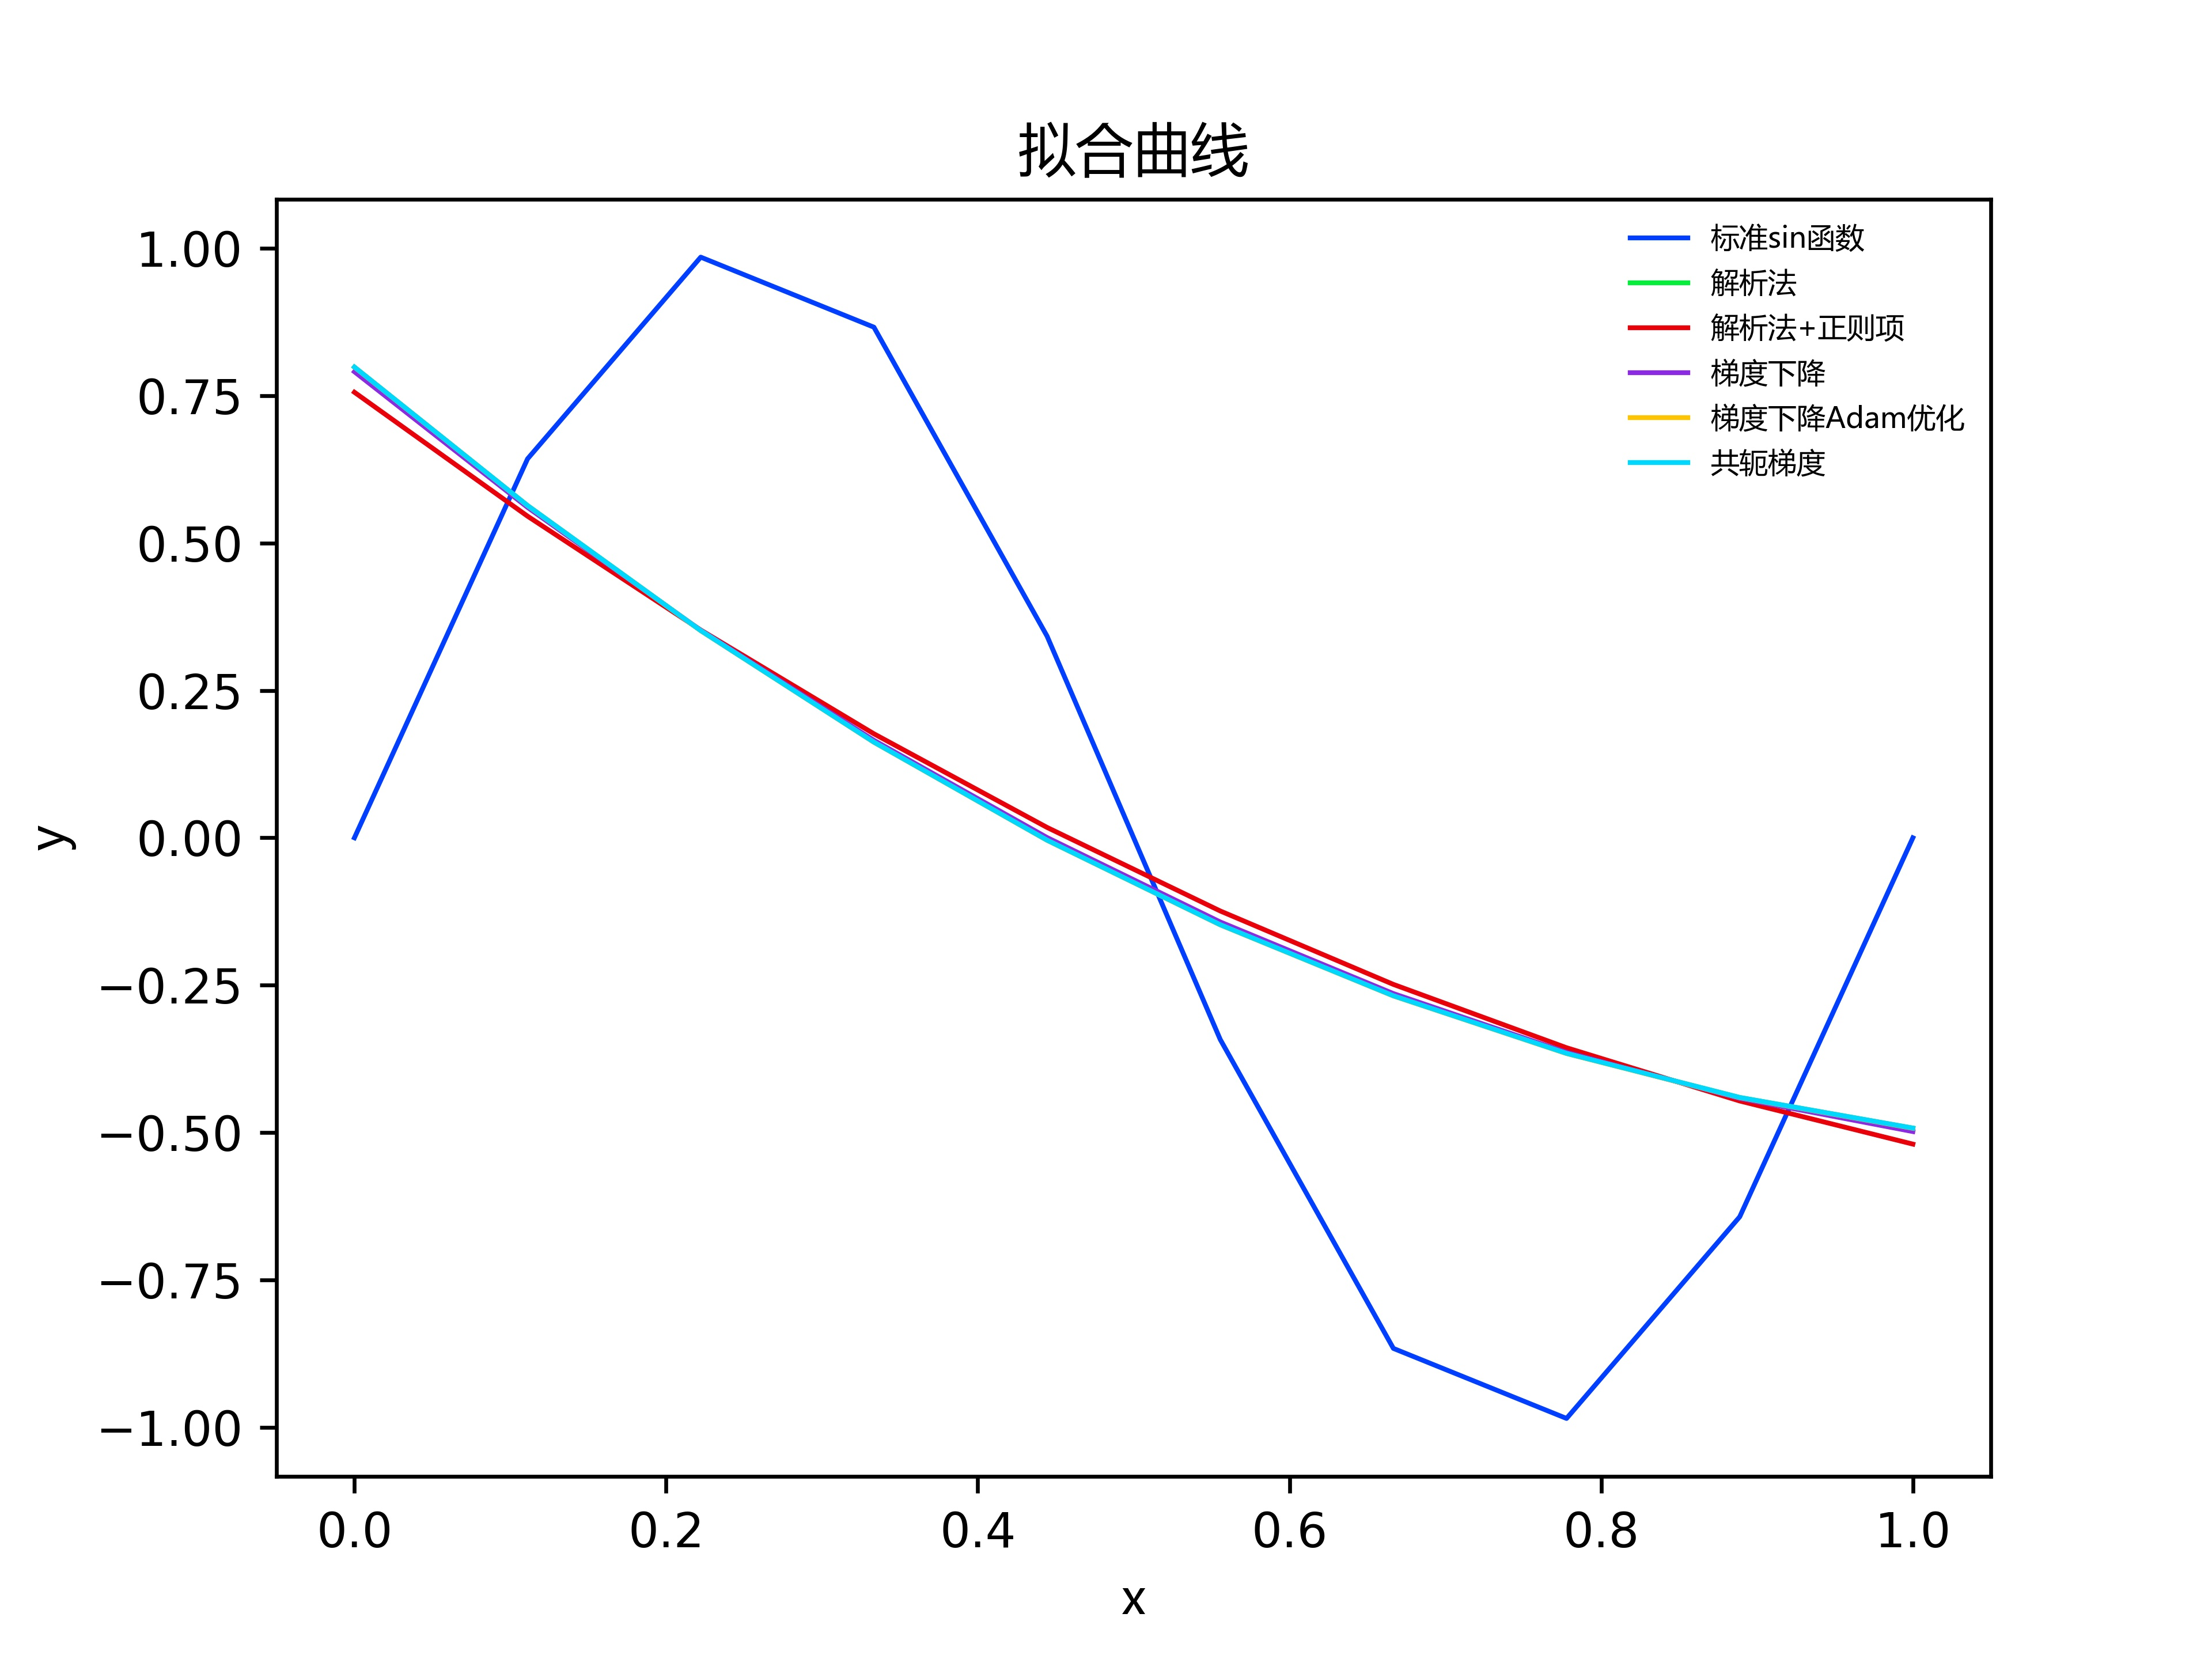
\includegraphics[width=0.3\textwidth]{n10o2}
}
\subfigure[3阶]{
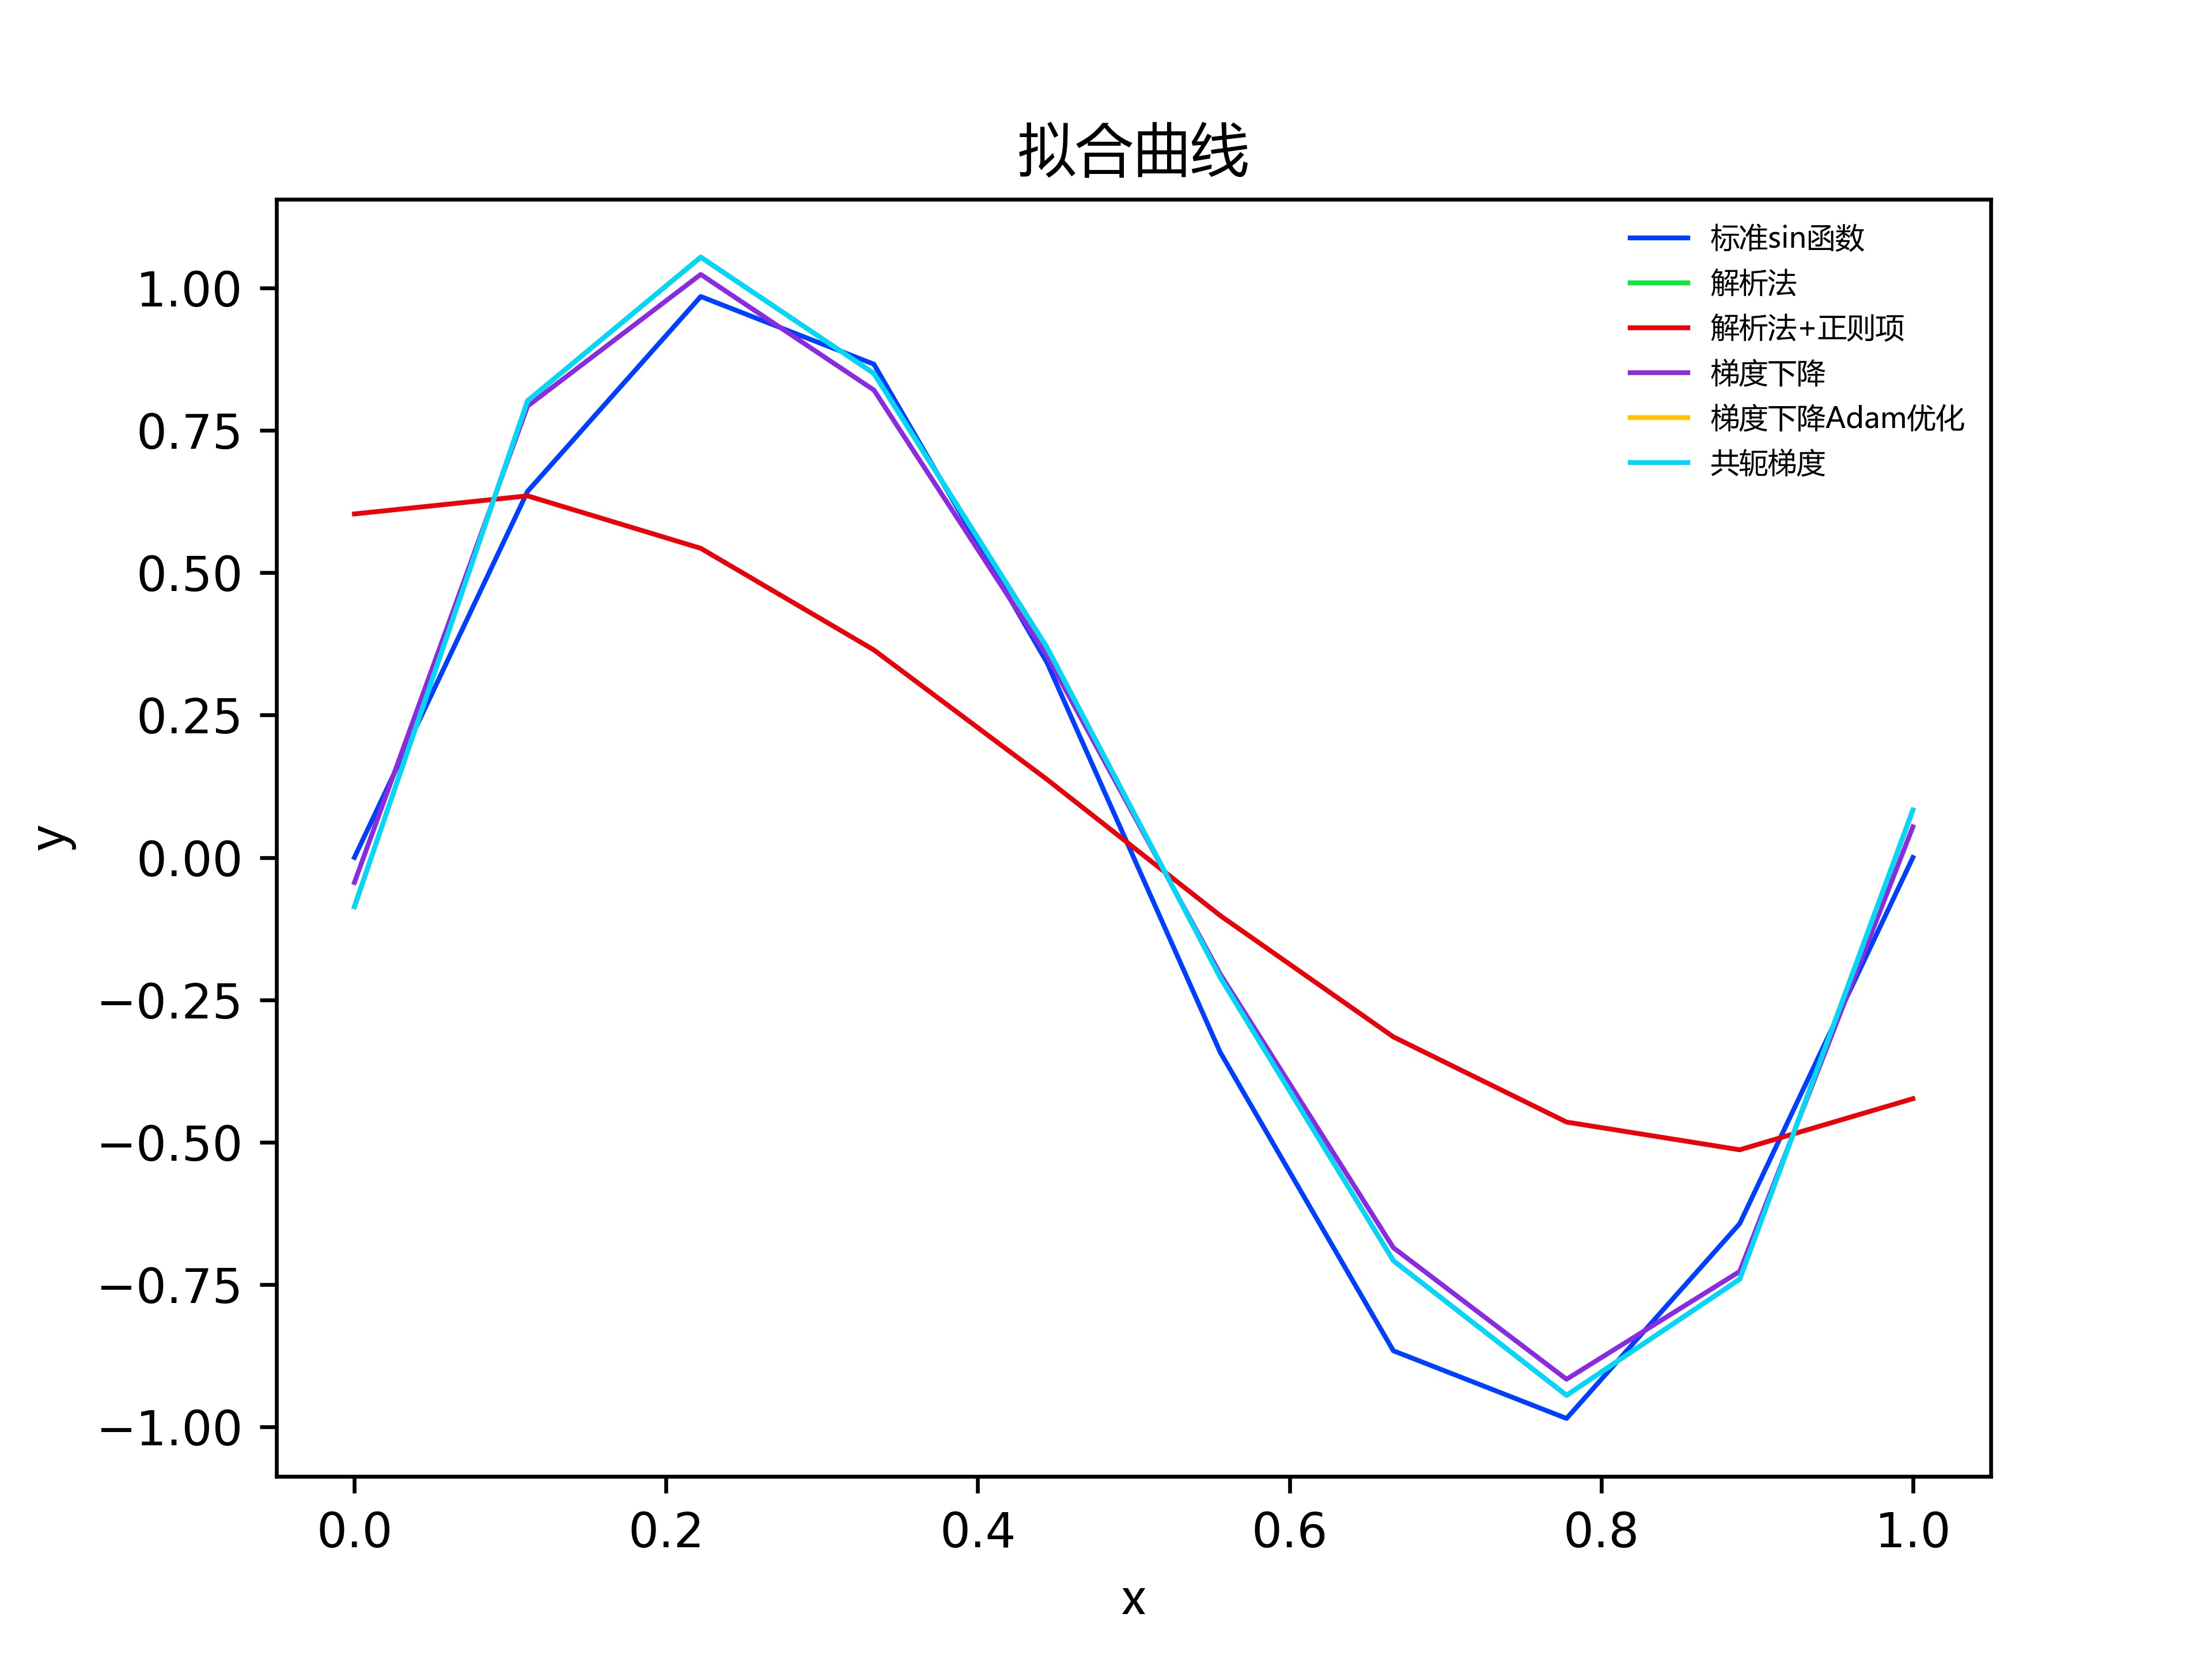
\includegraphics[width=0.3\textwidth]{n10o3}
}
\subfigure[5阶]{
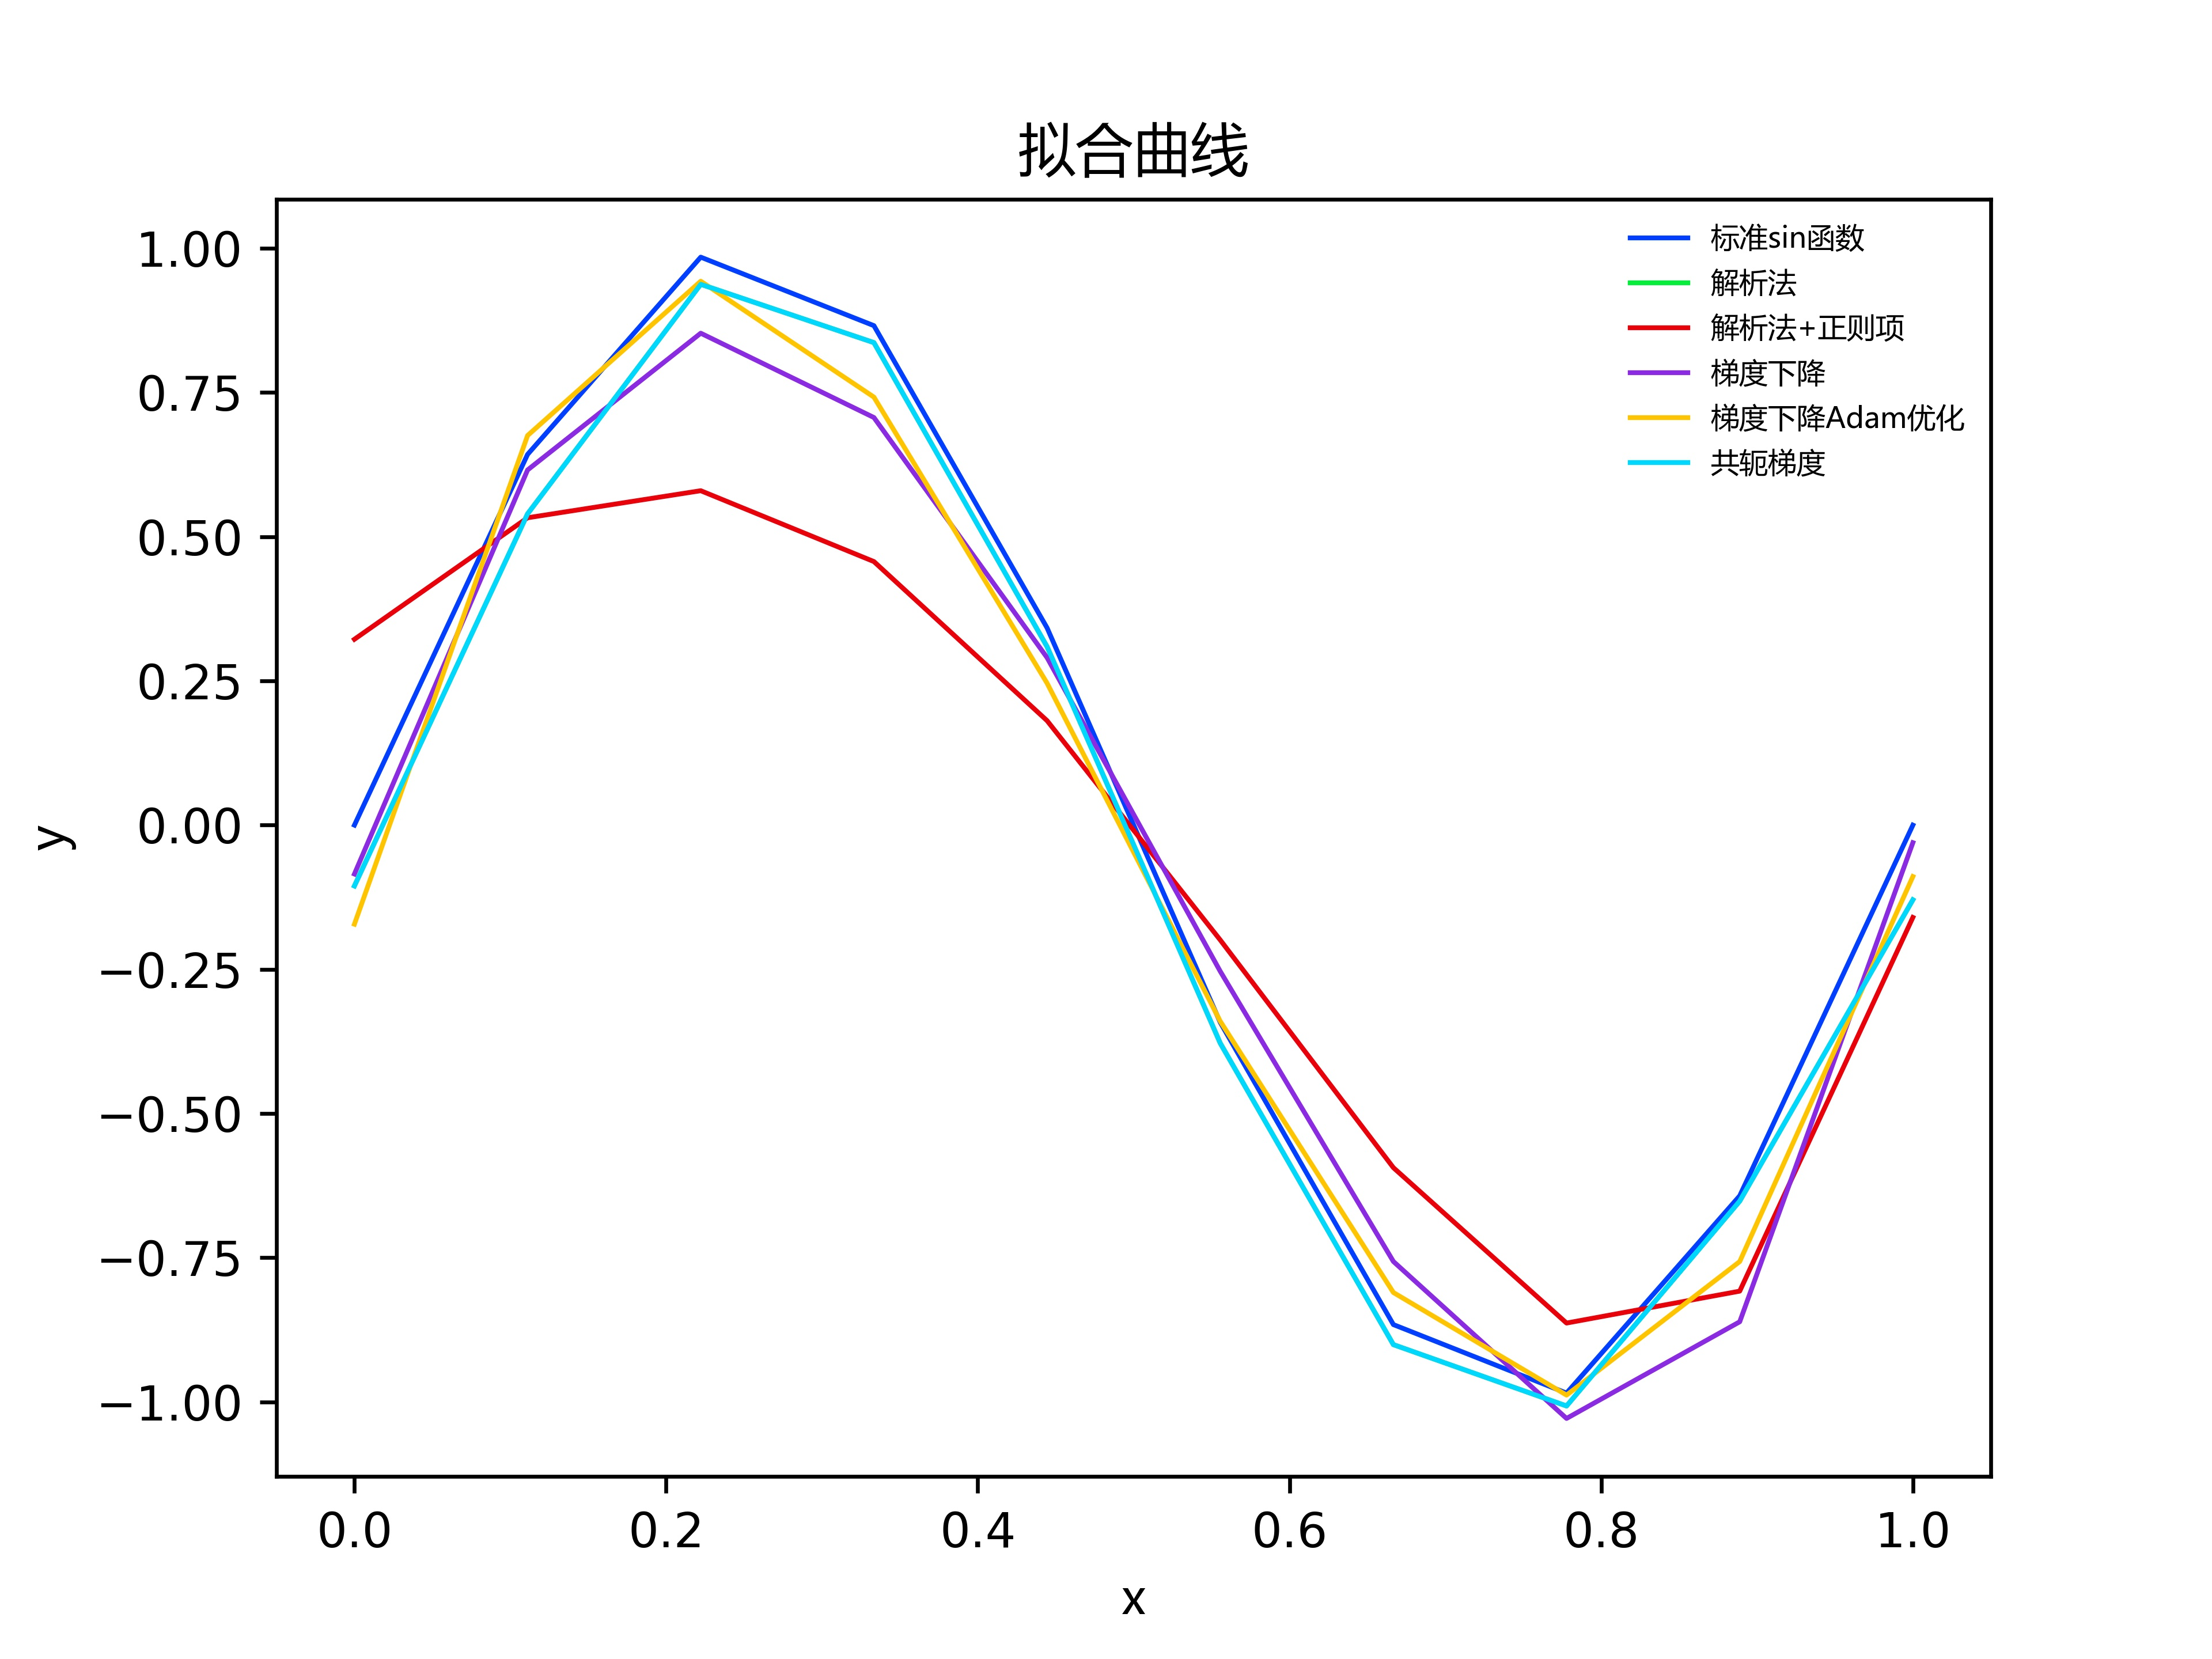
\includegraphics[width=0.3\textwidth]{n10o5}
}
\subfigure[7阶]{
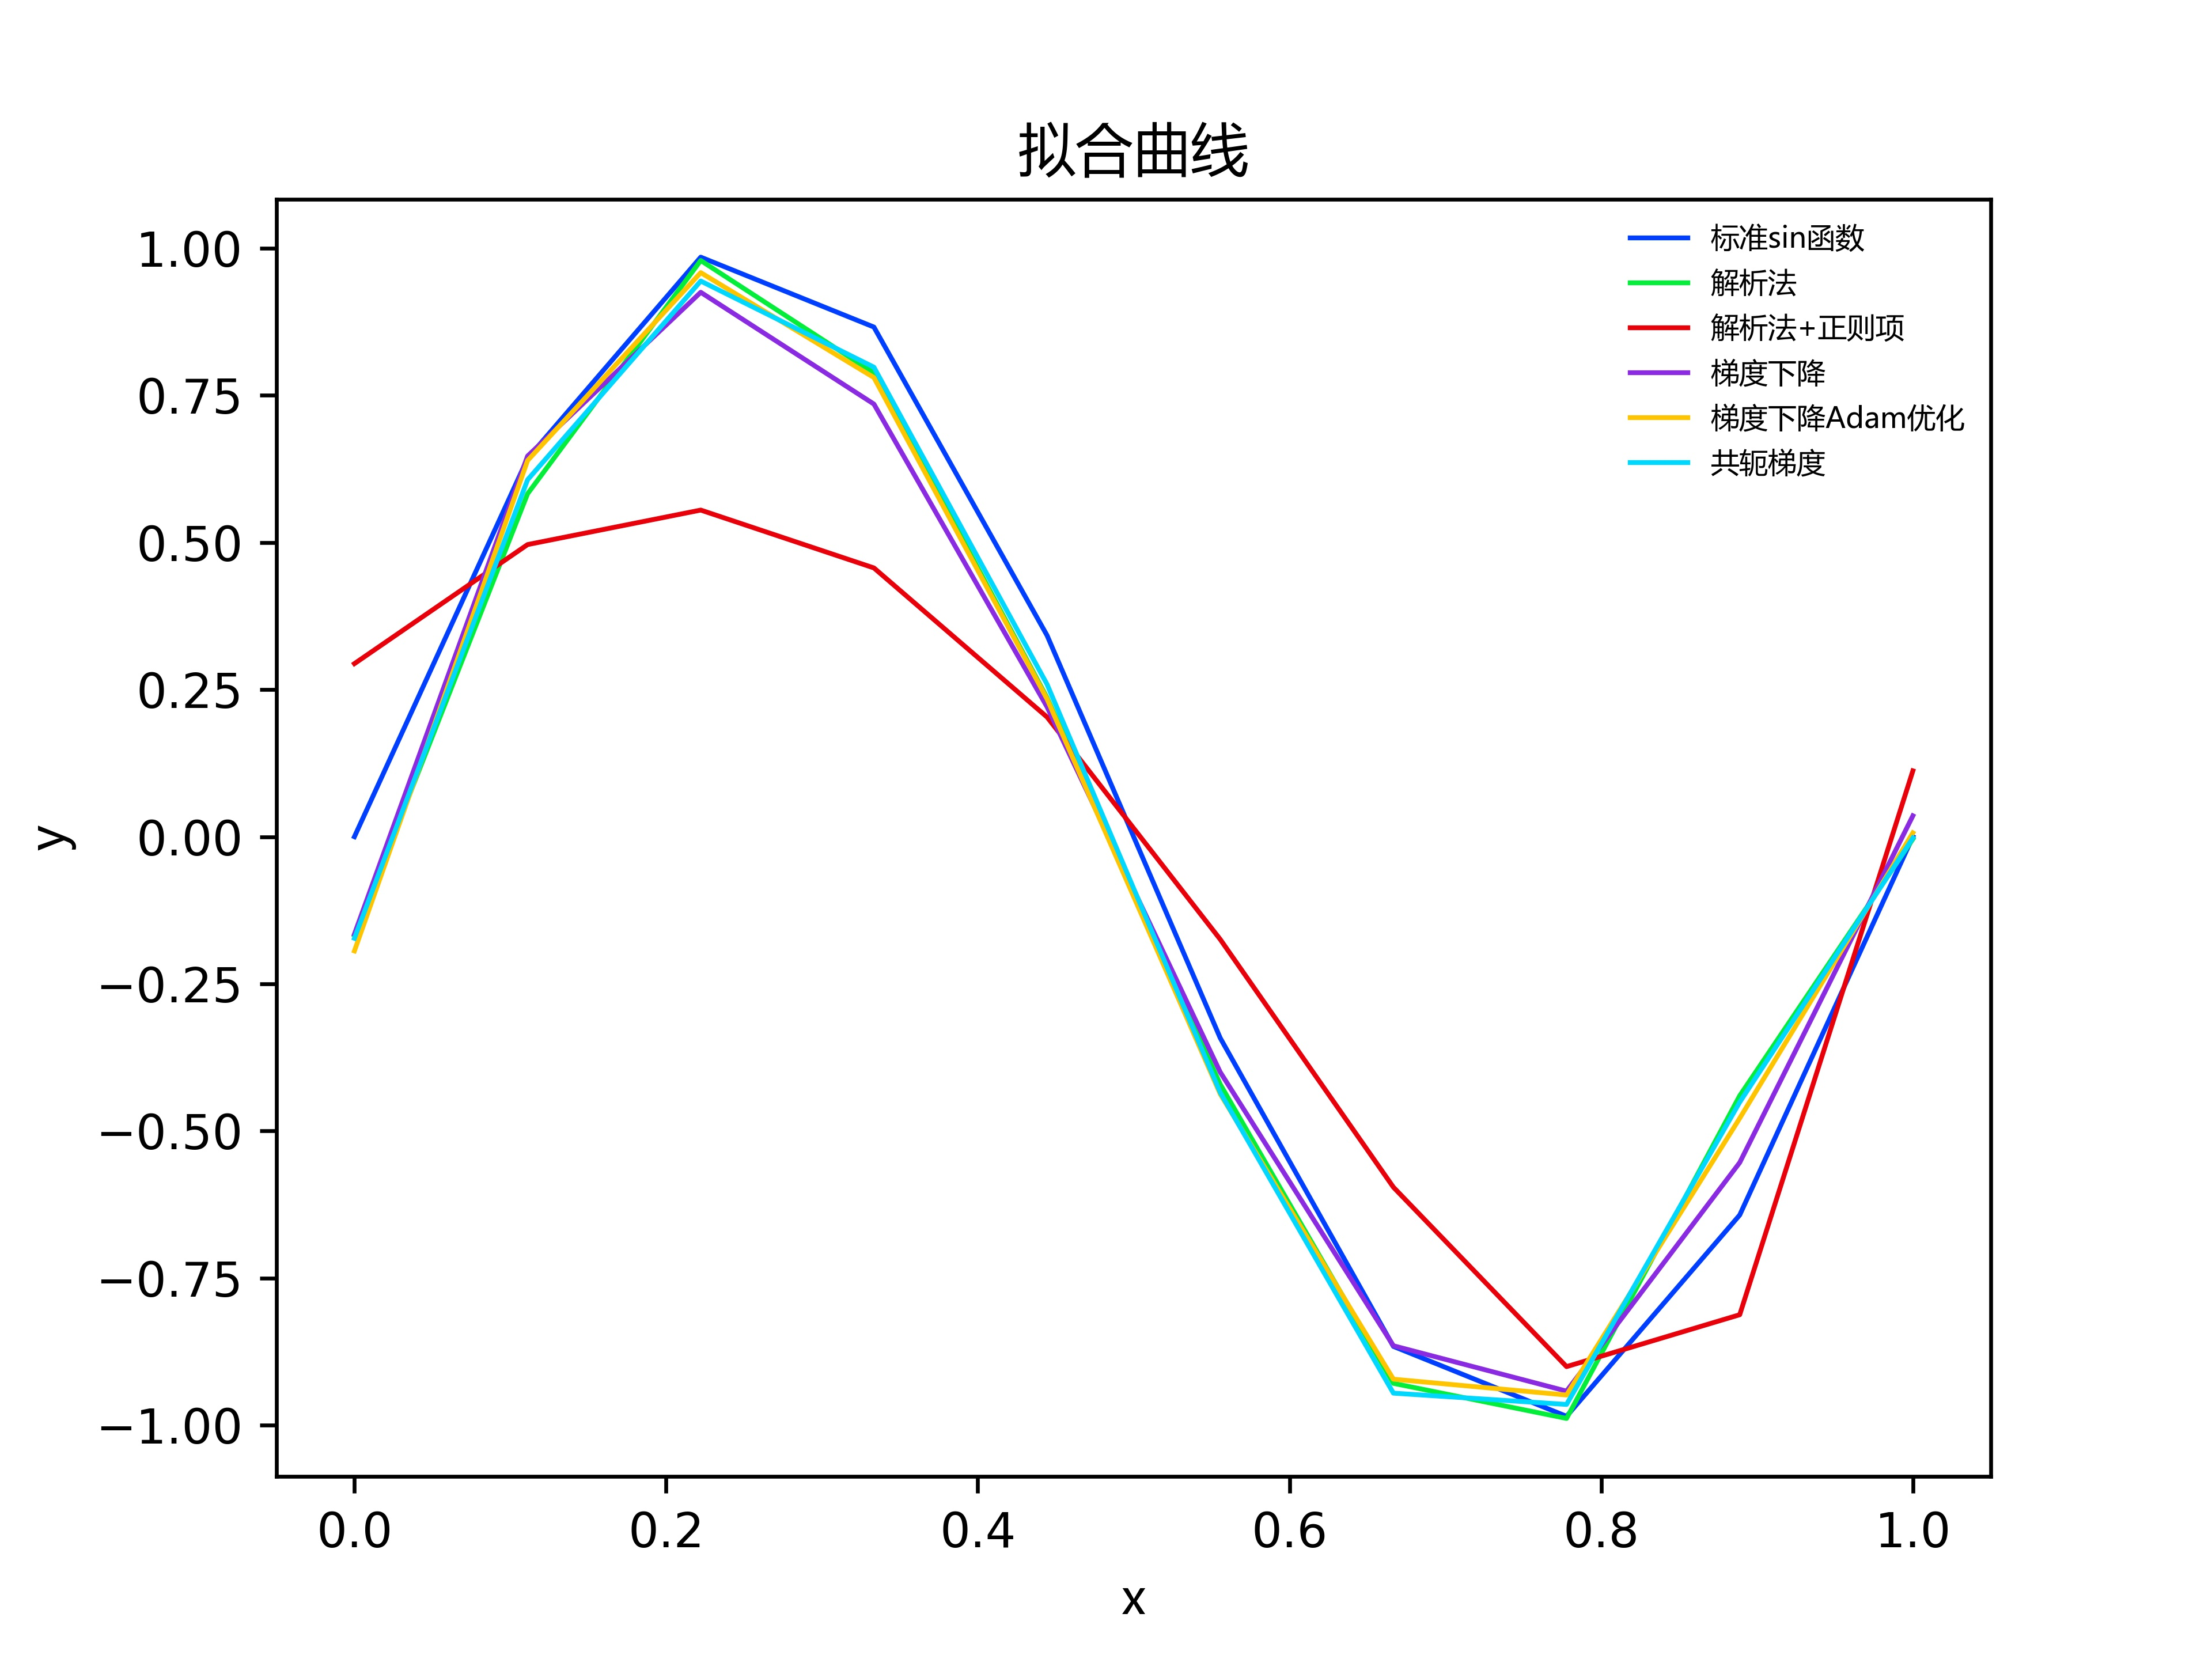
\includegraphics[width=0.3\textwidth]{n10o7}
}
\subfigure[8阶]{
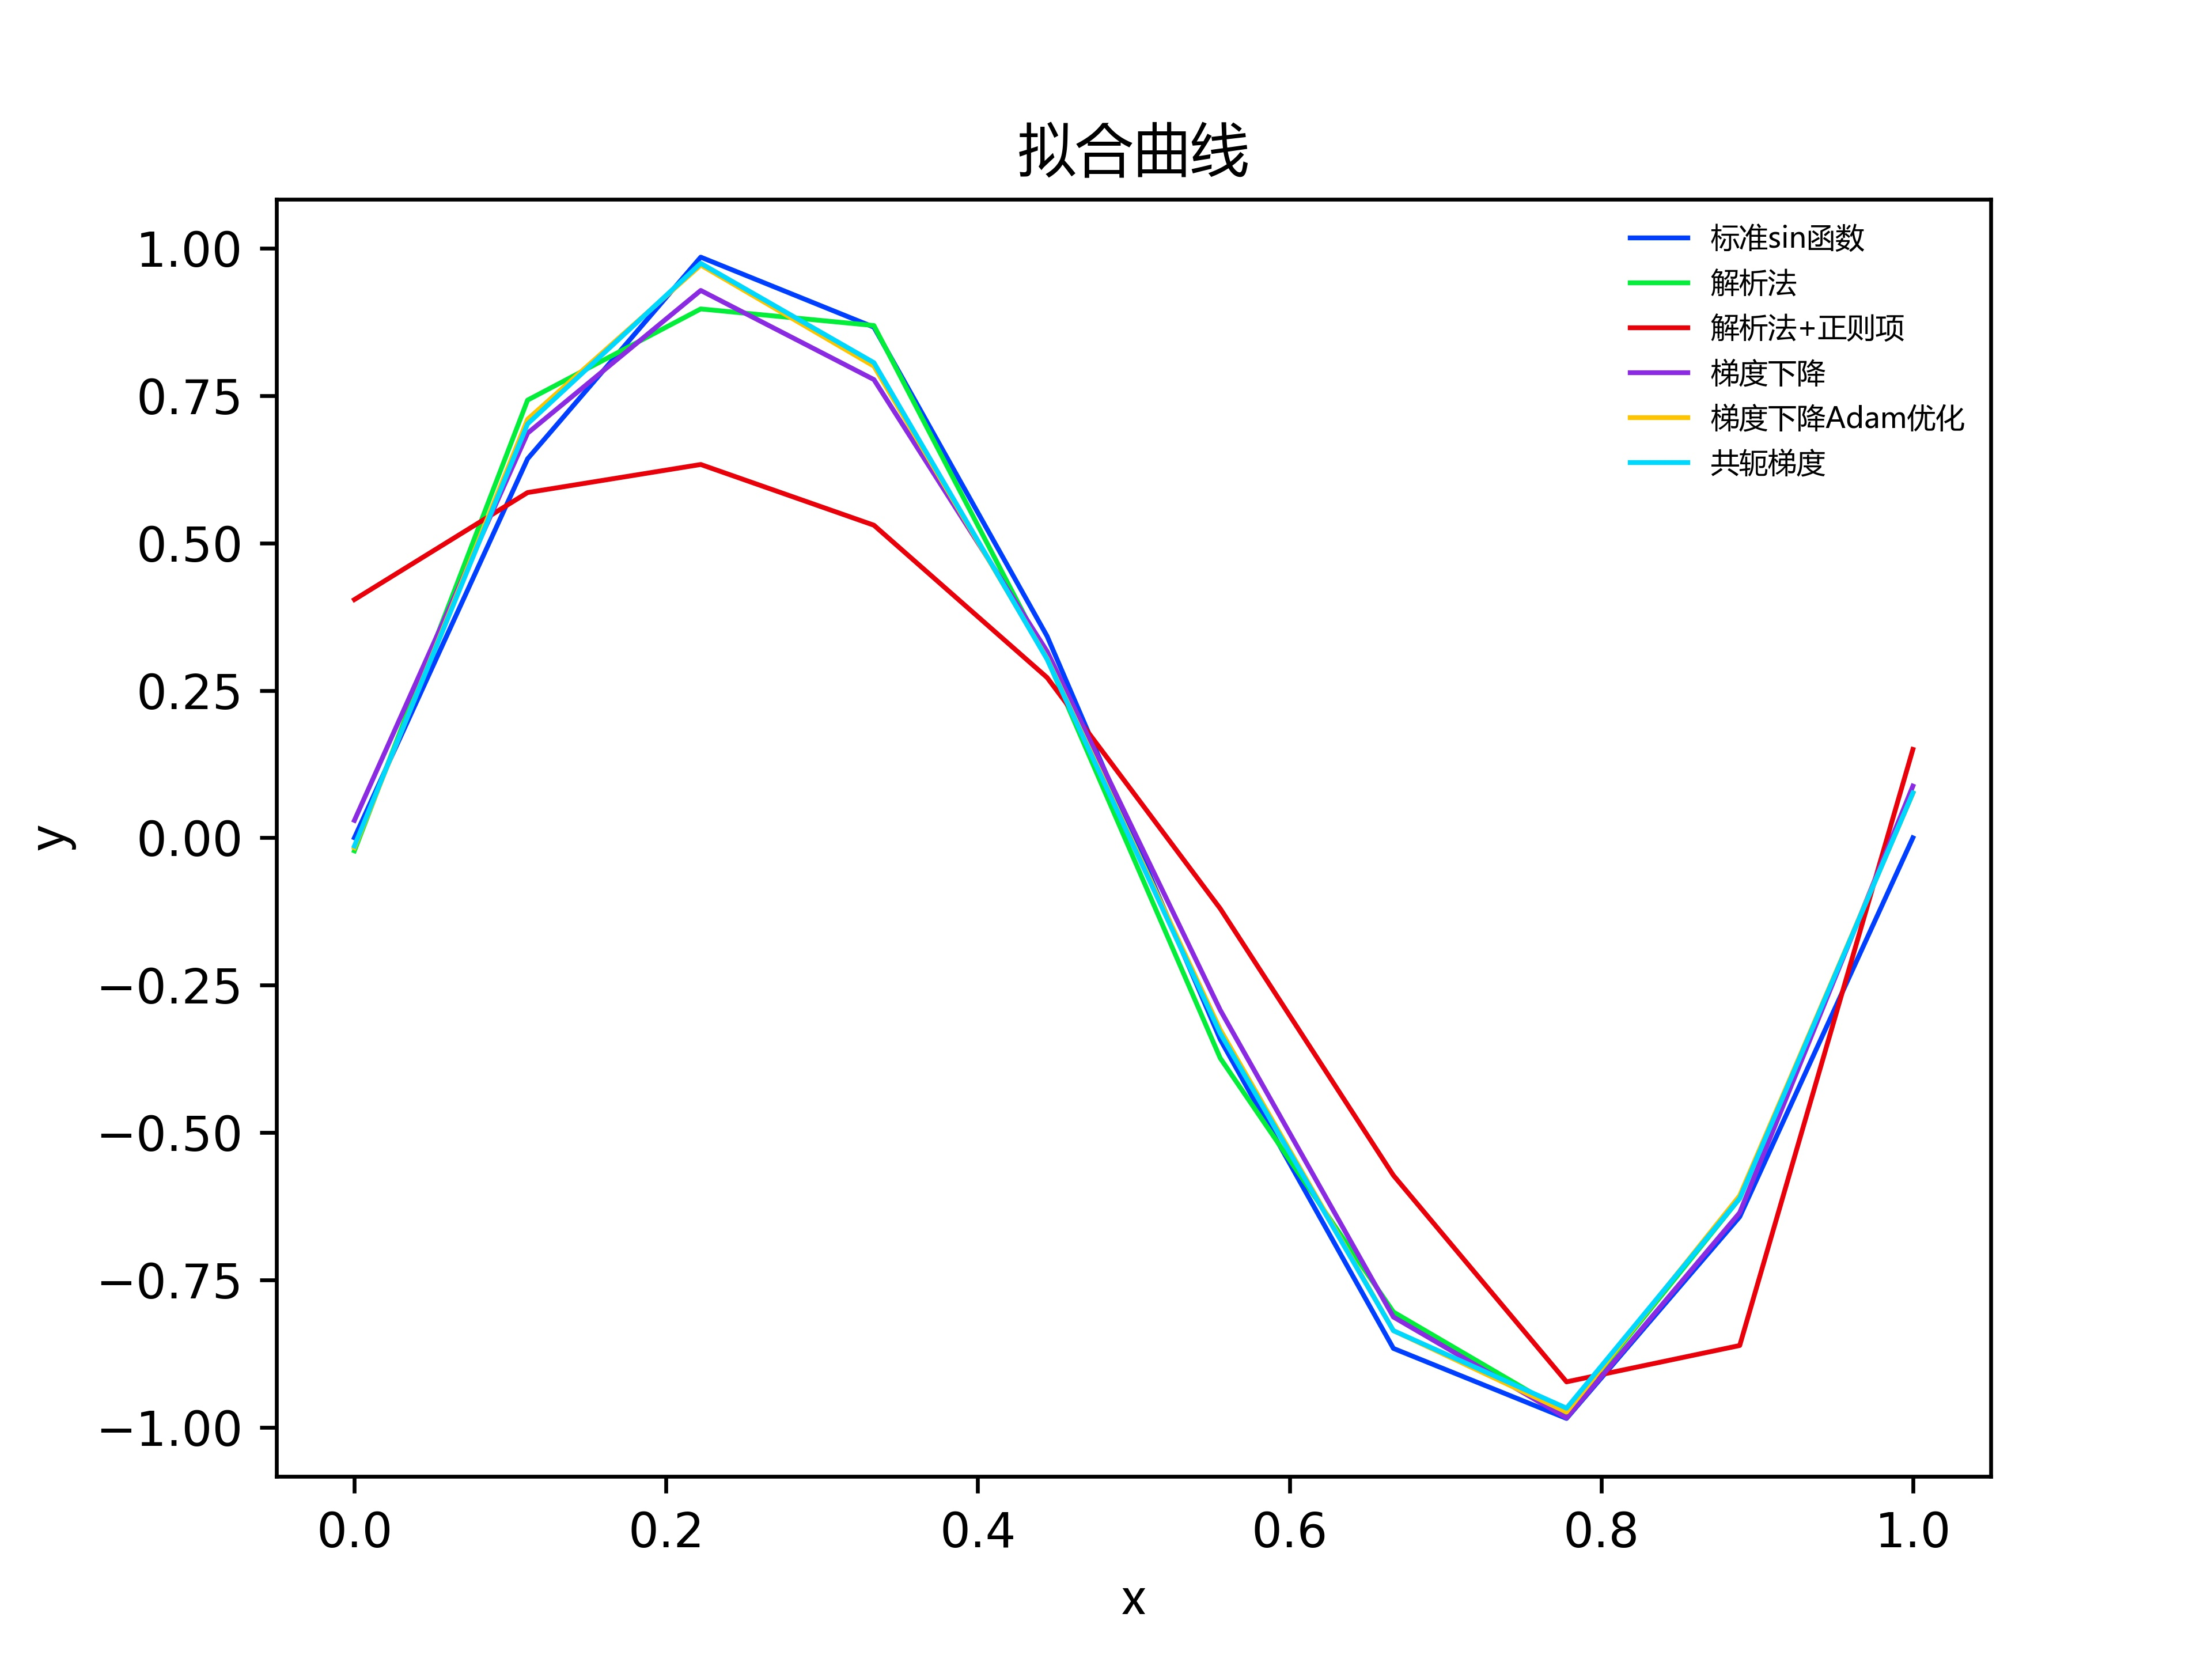
\includegraphics[width=0.3\textwidth]{n10o8}
}
\subfigure[9阶]{
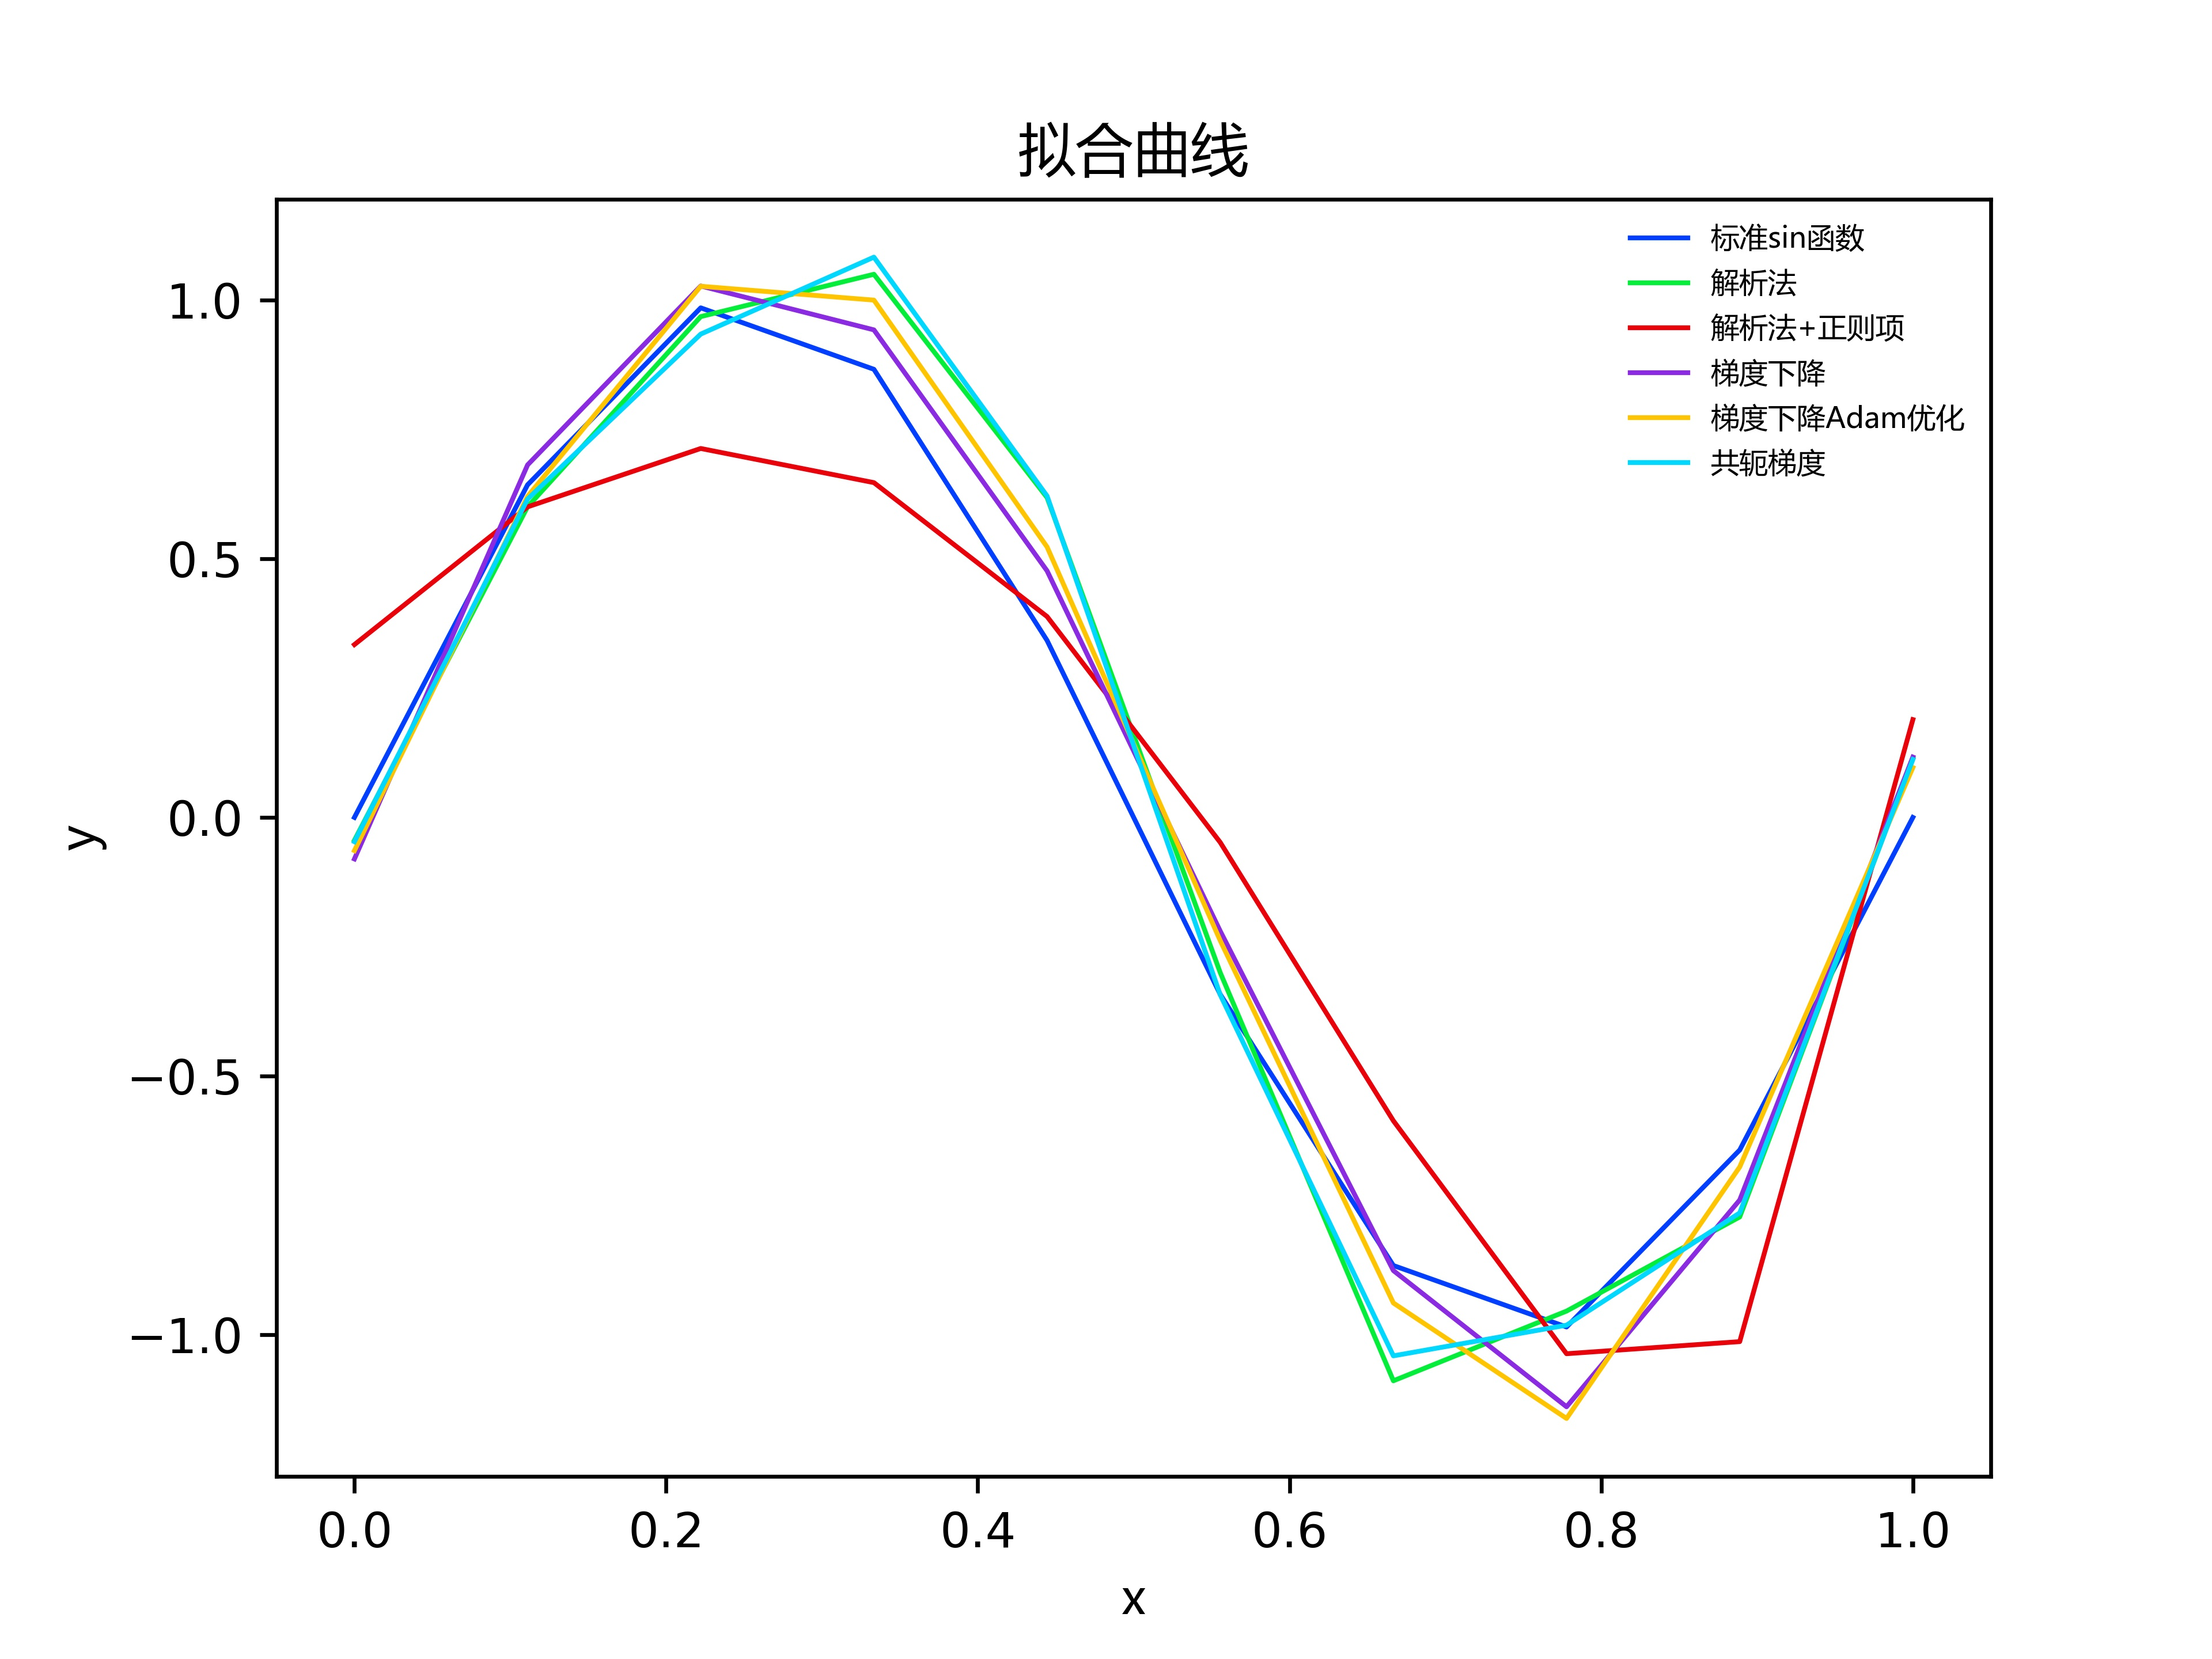
\includegraphics[width=0.3\textwidth]{n10o9}
}
\caption{n=10 不同阶拟合曲线}
\end{figure}

观察实验结果,除因正则项系数过大而导致过于平缓,其他方法均拟合较好。但阶数为2的情况下,多项式式拟合能力过差,拟合曲线偏差较大。随着阶数的增加,拟合优度大体上均先降后增,在阶数为8的情况下拟合效果最好。

\newpage
当数据集大小为20时,取多项式阶数为2,3,5,7,8,9。其拟合曲线及拟合优度如下。

\linespread{1.2}
\begin{table}[H]  
  \centering  
  \begin{threeparttable}  
  \caption{n=20 不同阶拟合优度}
  \label{tab:performance_comparison} 
  \begin{tabular}{m{0.1\textwidth}<{\centering} m{0.15\textwidth}<{\centering} m{0.15\textwidth}<{\centering} m{0.15\textwidth}<{\centering} m{0.15\textwidth}<{\centering} m{0.15\textwidth}<{\centering}}  
    \toprule[1.5pt]  
    \multirow{2}{*}{阶数}&\multicolumn{2}{c}{解析法}&\multicolumn{2}{c}{梯度下降} &\multirow{2}{*}{共轭梯度}\cr  
    \cmidrule(lr){2-3} \cmidrule(lr){4-5}  
    &不含正则项&含正则项&未优化&优化后\cr  
    \midrule  
2&0.6819&0.6818&0.6819&0.6819&0.6819\cr
3&0.1265&0.4760&0.1175&0.1265&0.1265\cr
5&0.0444&0.2797&0.1689&0.0914&0.0444\cr
7&0.0614&0.2959&0.0771&0.0548&0.0498\cr
8&0.0785&0.3047&0.1003&0.0820&0.0769\cr
9&0.0947&0.2757&0.0640&0.0728&0.0923\cr
    \bottomrule  
    \end{tabular}  
    \end{threeparttable}  
\end{table}

\begin{figure}[H]
\centering
\subfigure[2阶]{
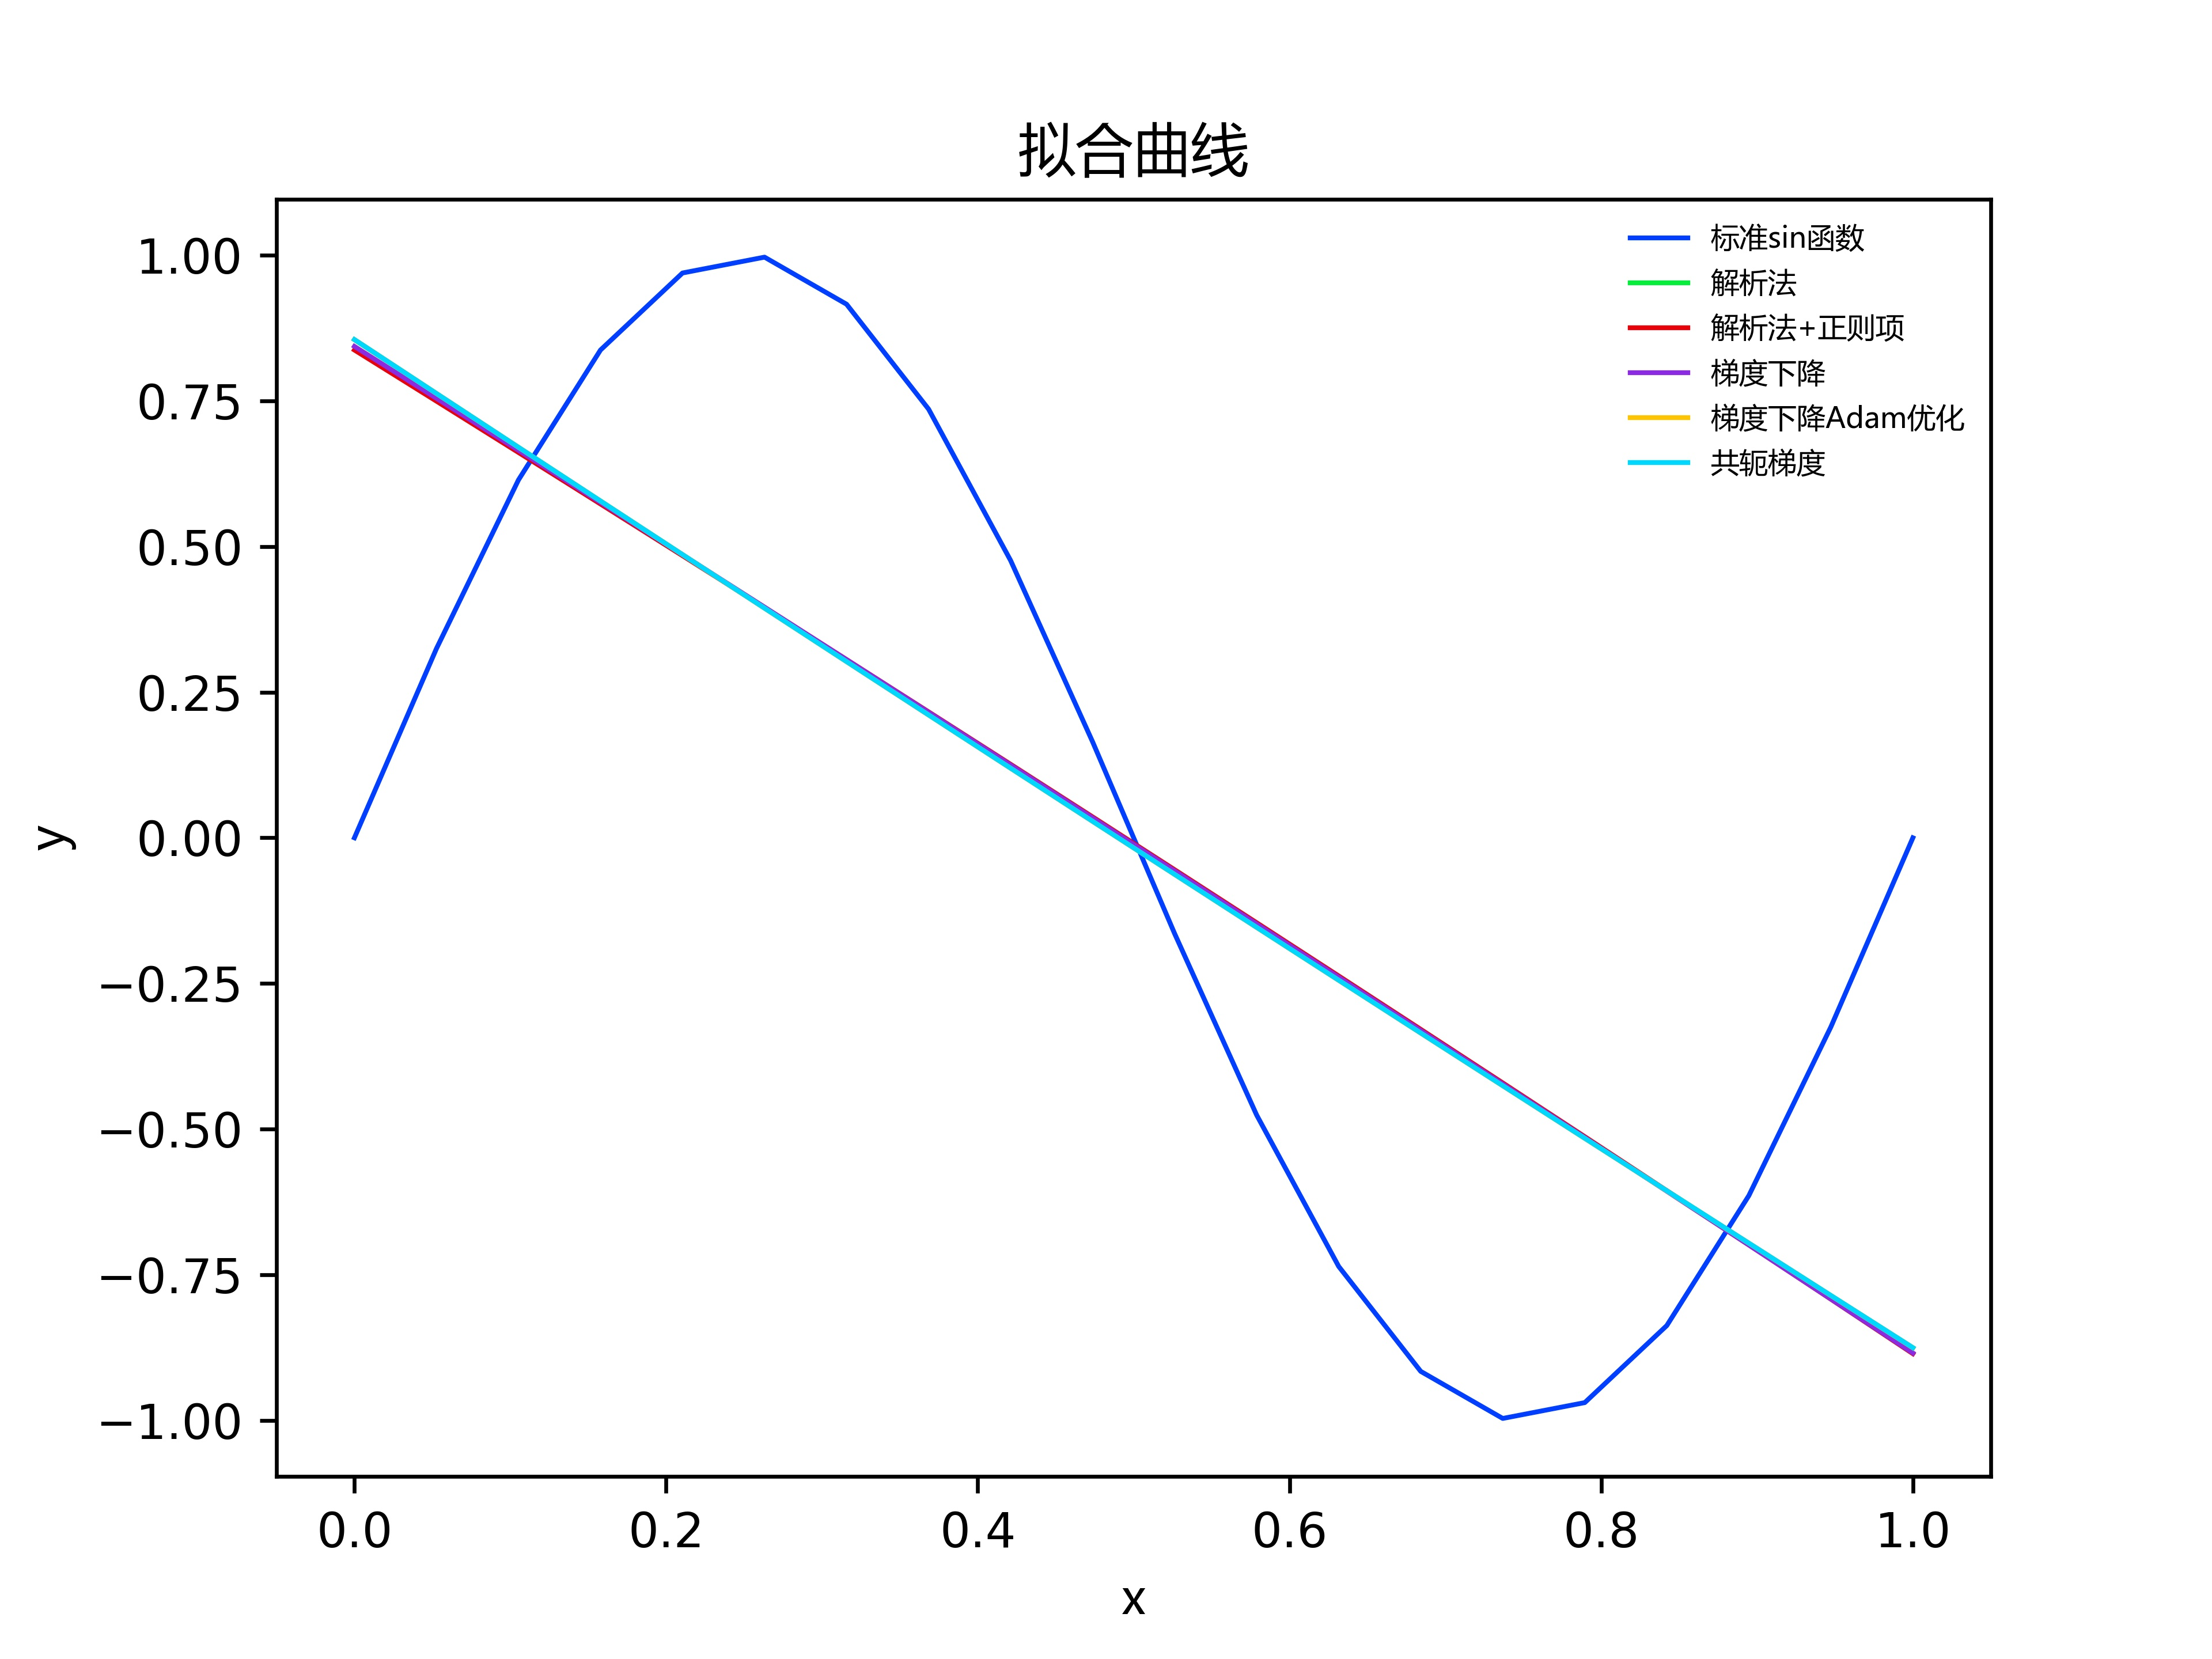
\includegraphics[width=0.3\textwidth]{n20o2}
}
\subfigure[3阶]{
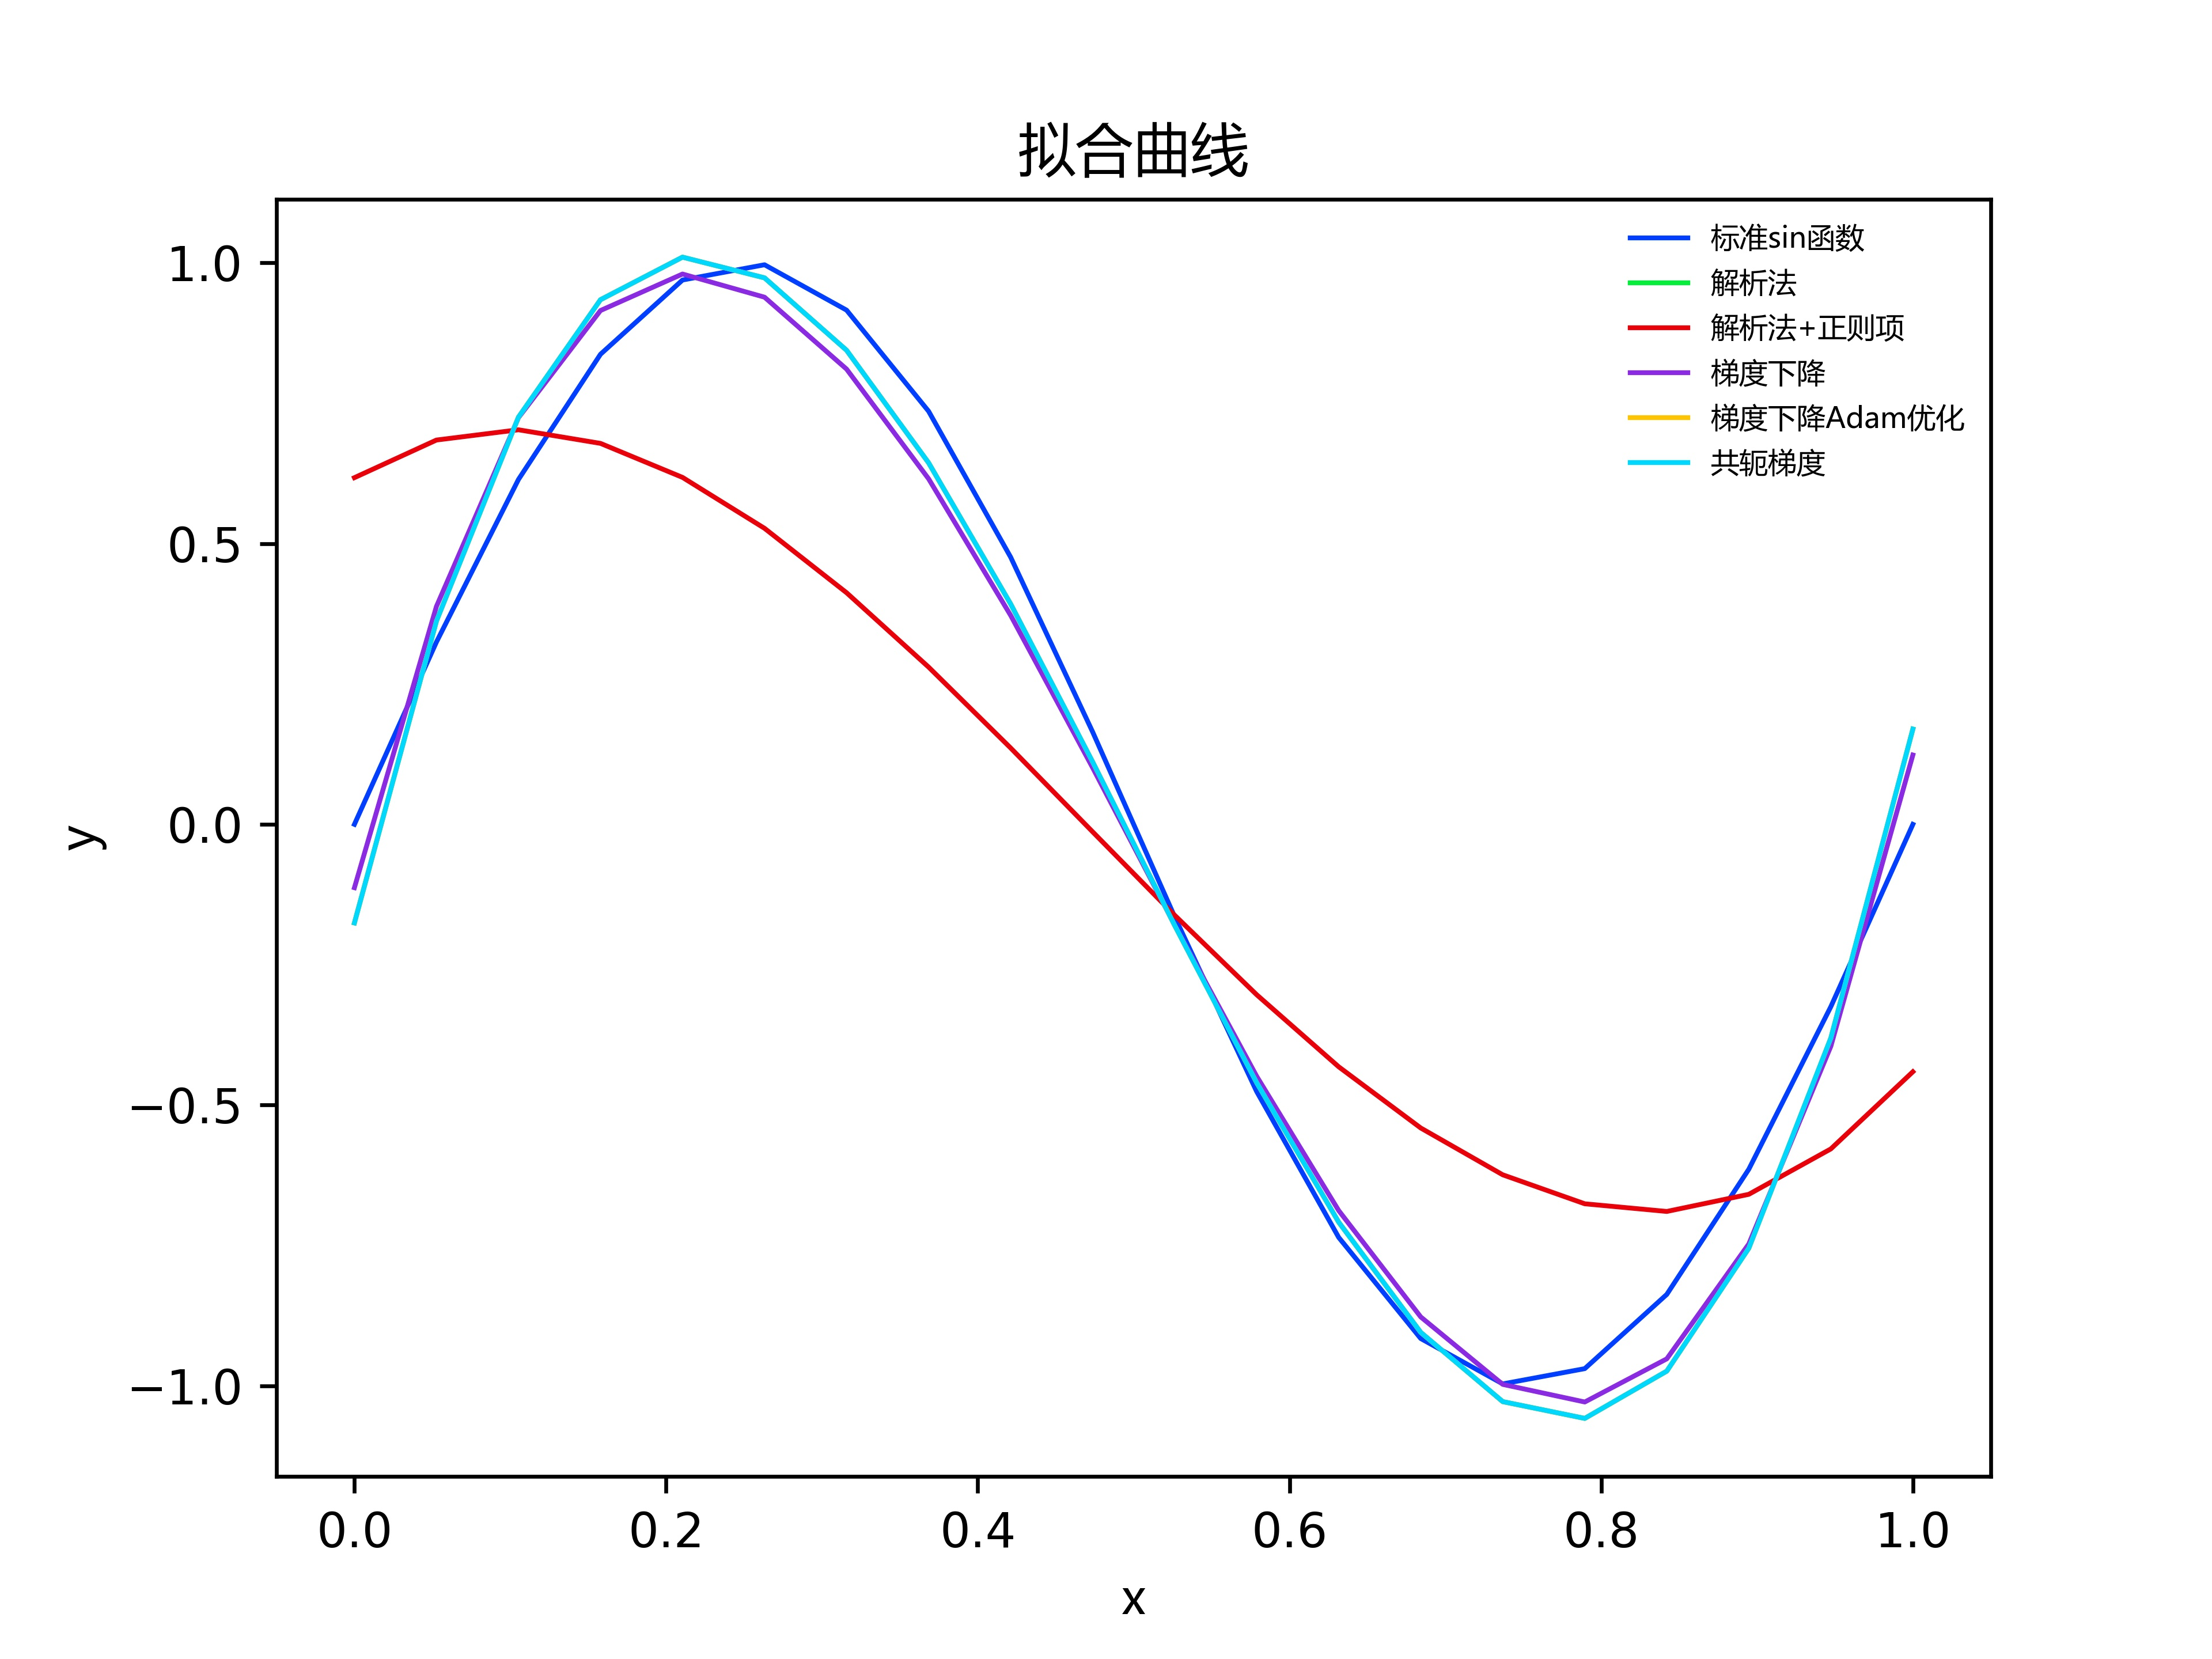
\includegraphics[width=0.3\textwidth]{n20o3}
}
\subfigure[5阶]{
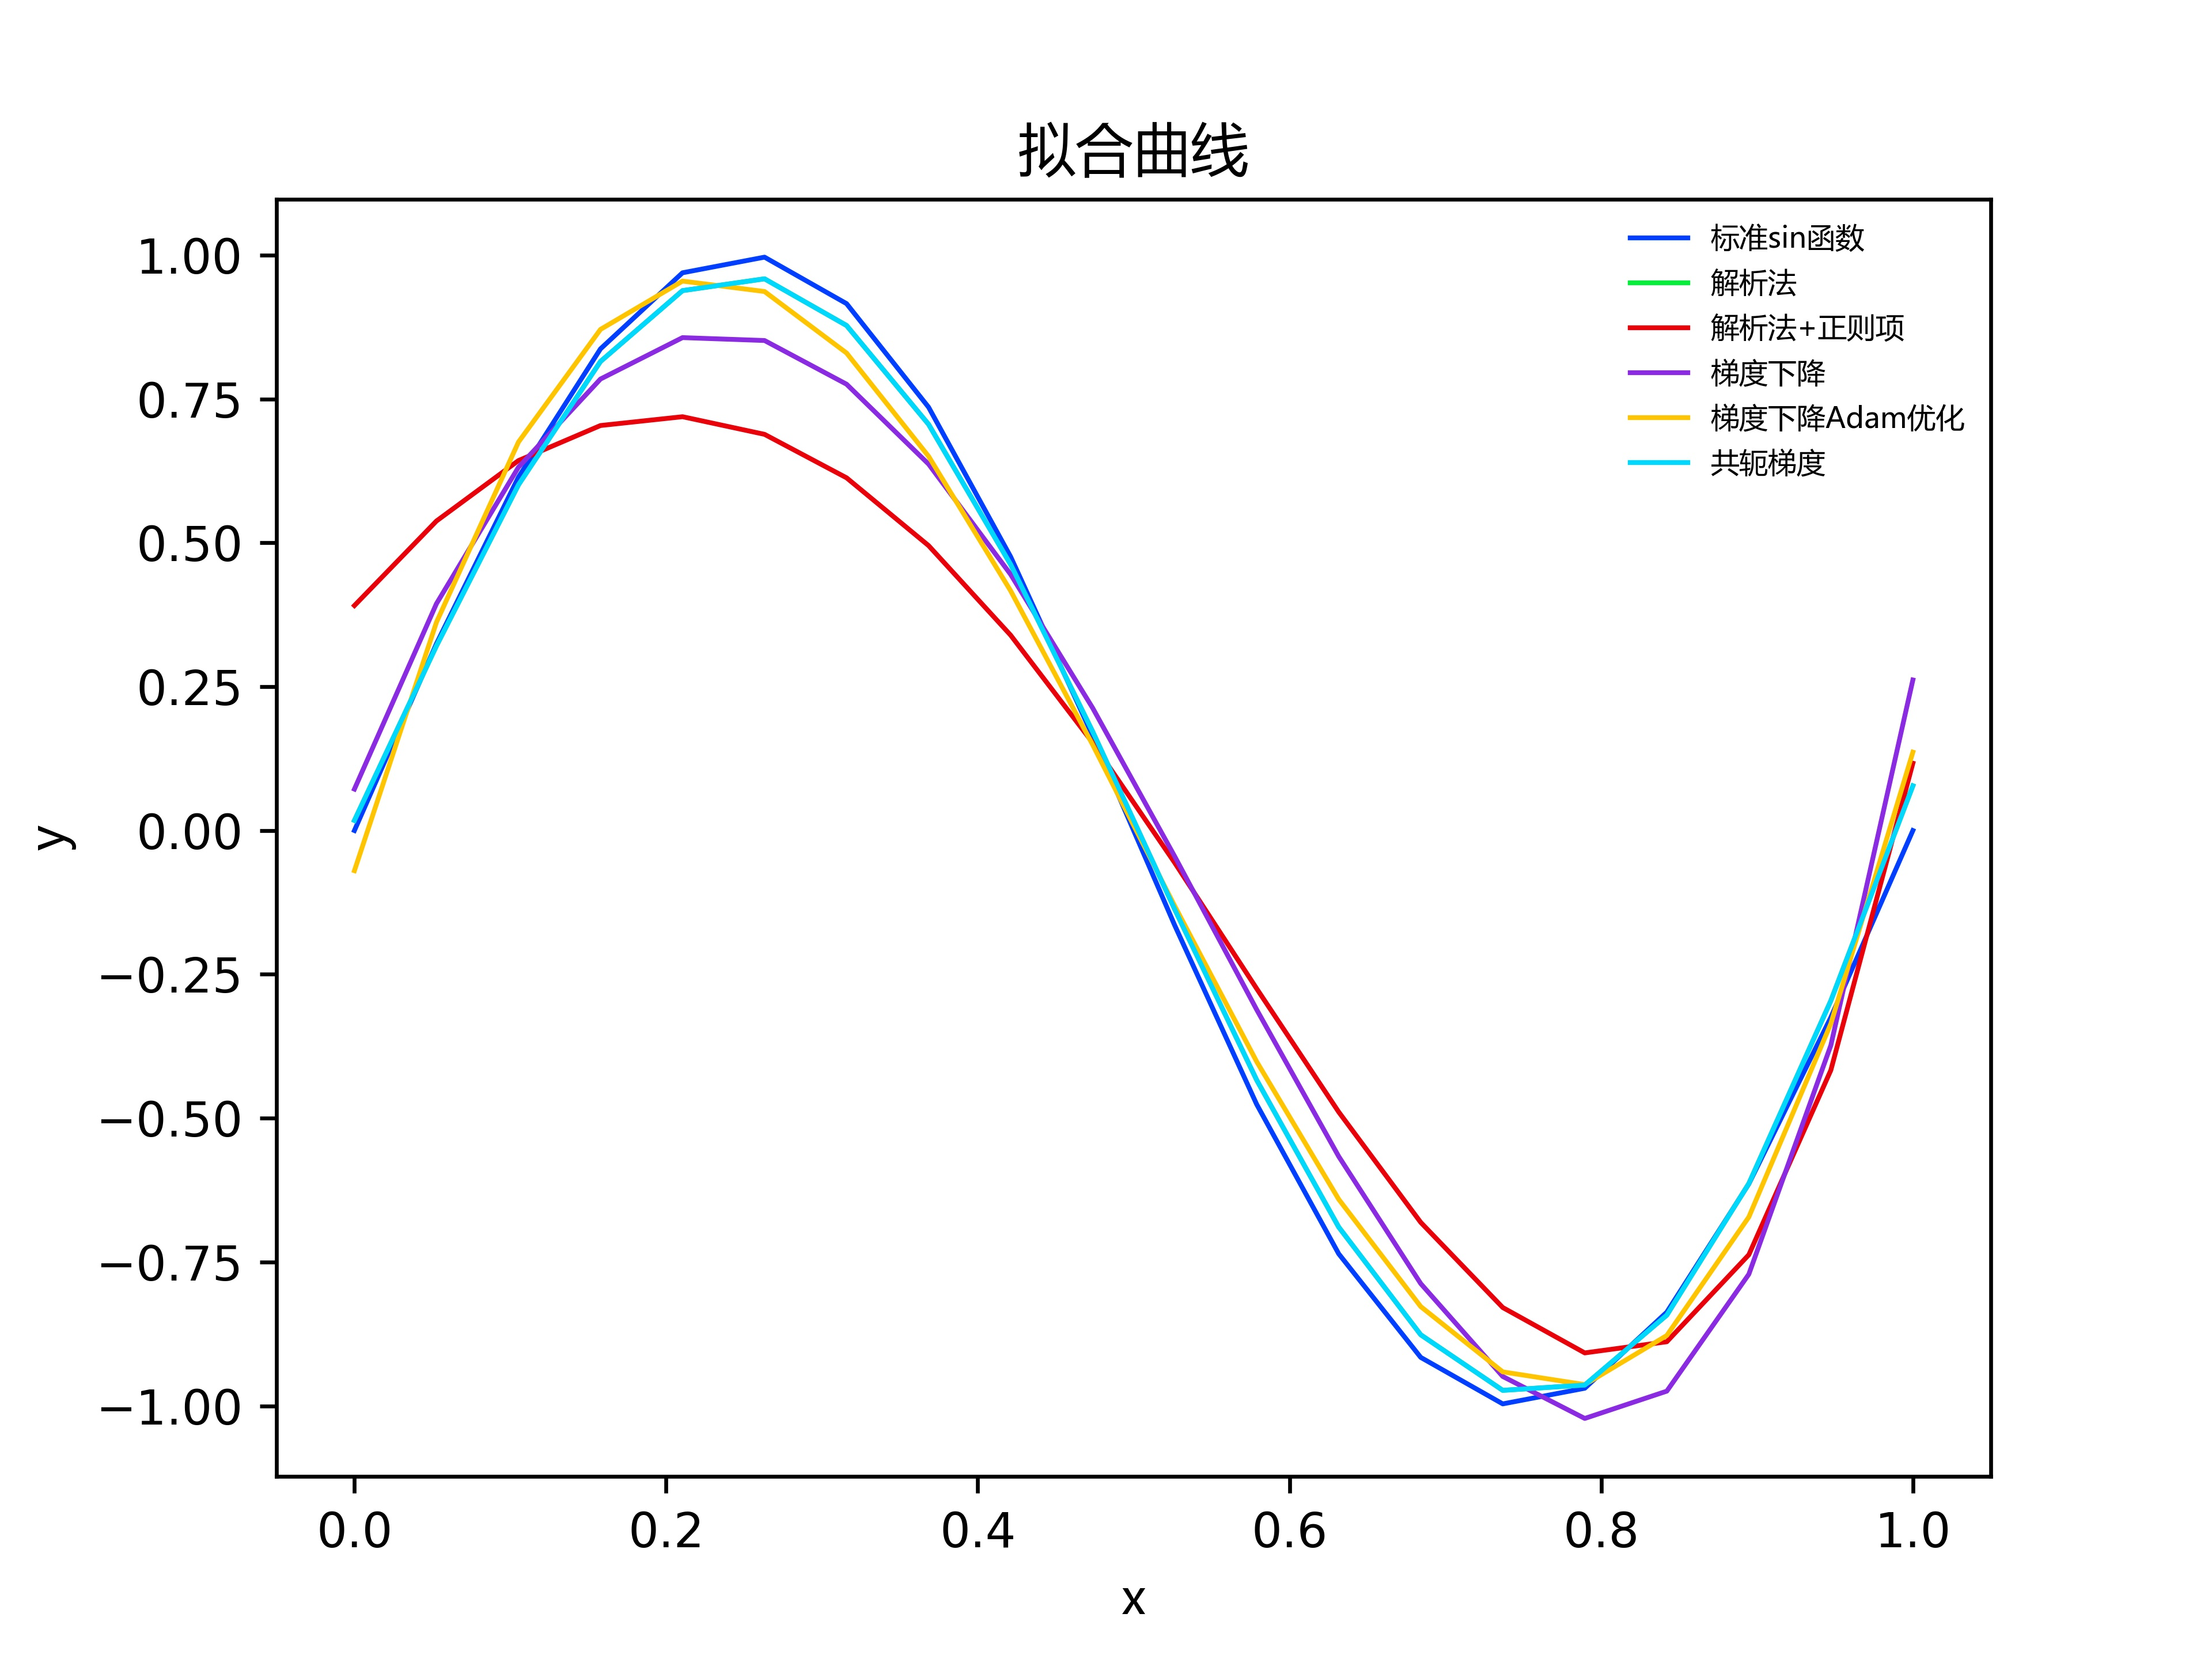
\includegraphics[width=0.3\textwidth]{n20o5}
}
\quad
\subfigure[7阶]{
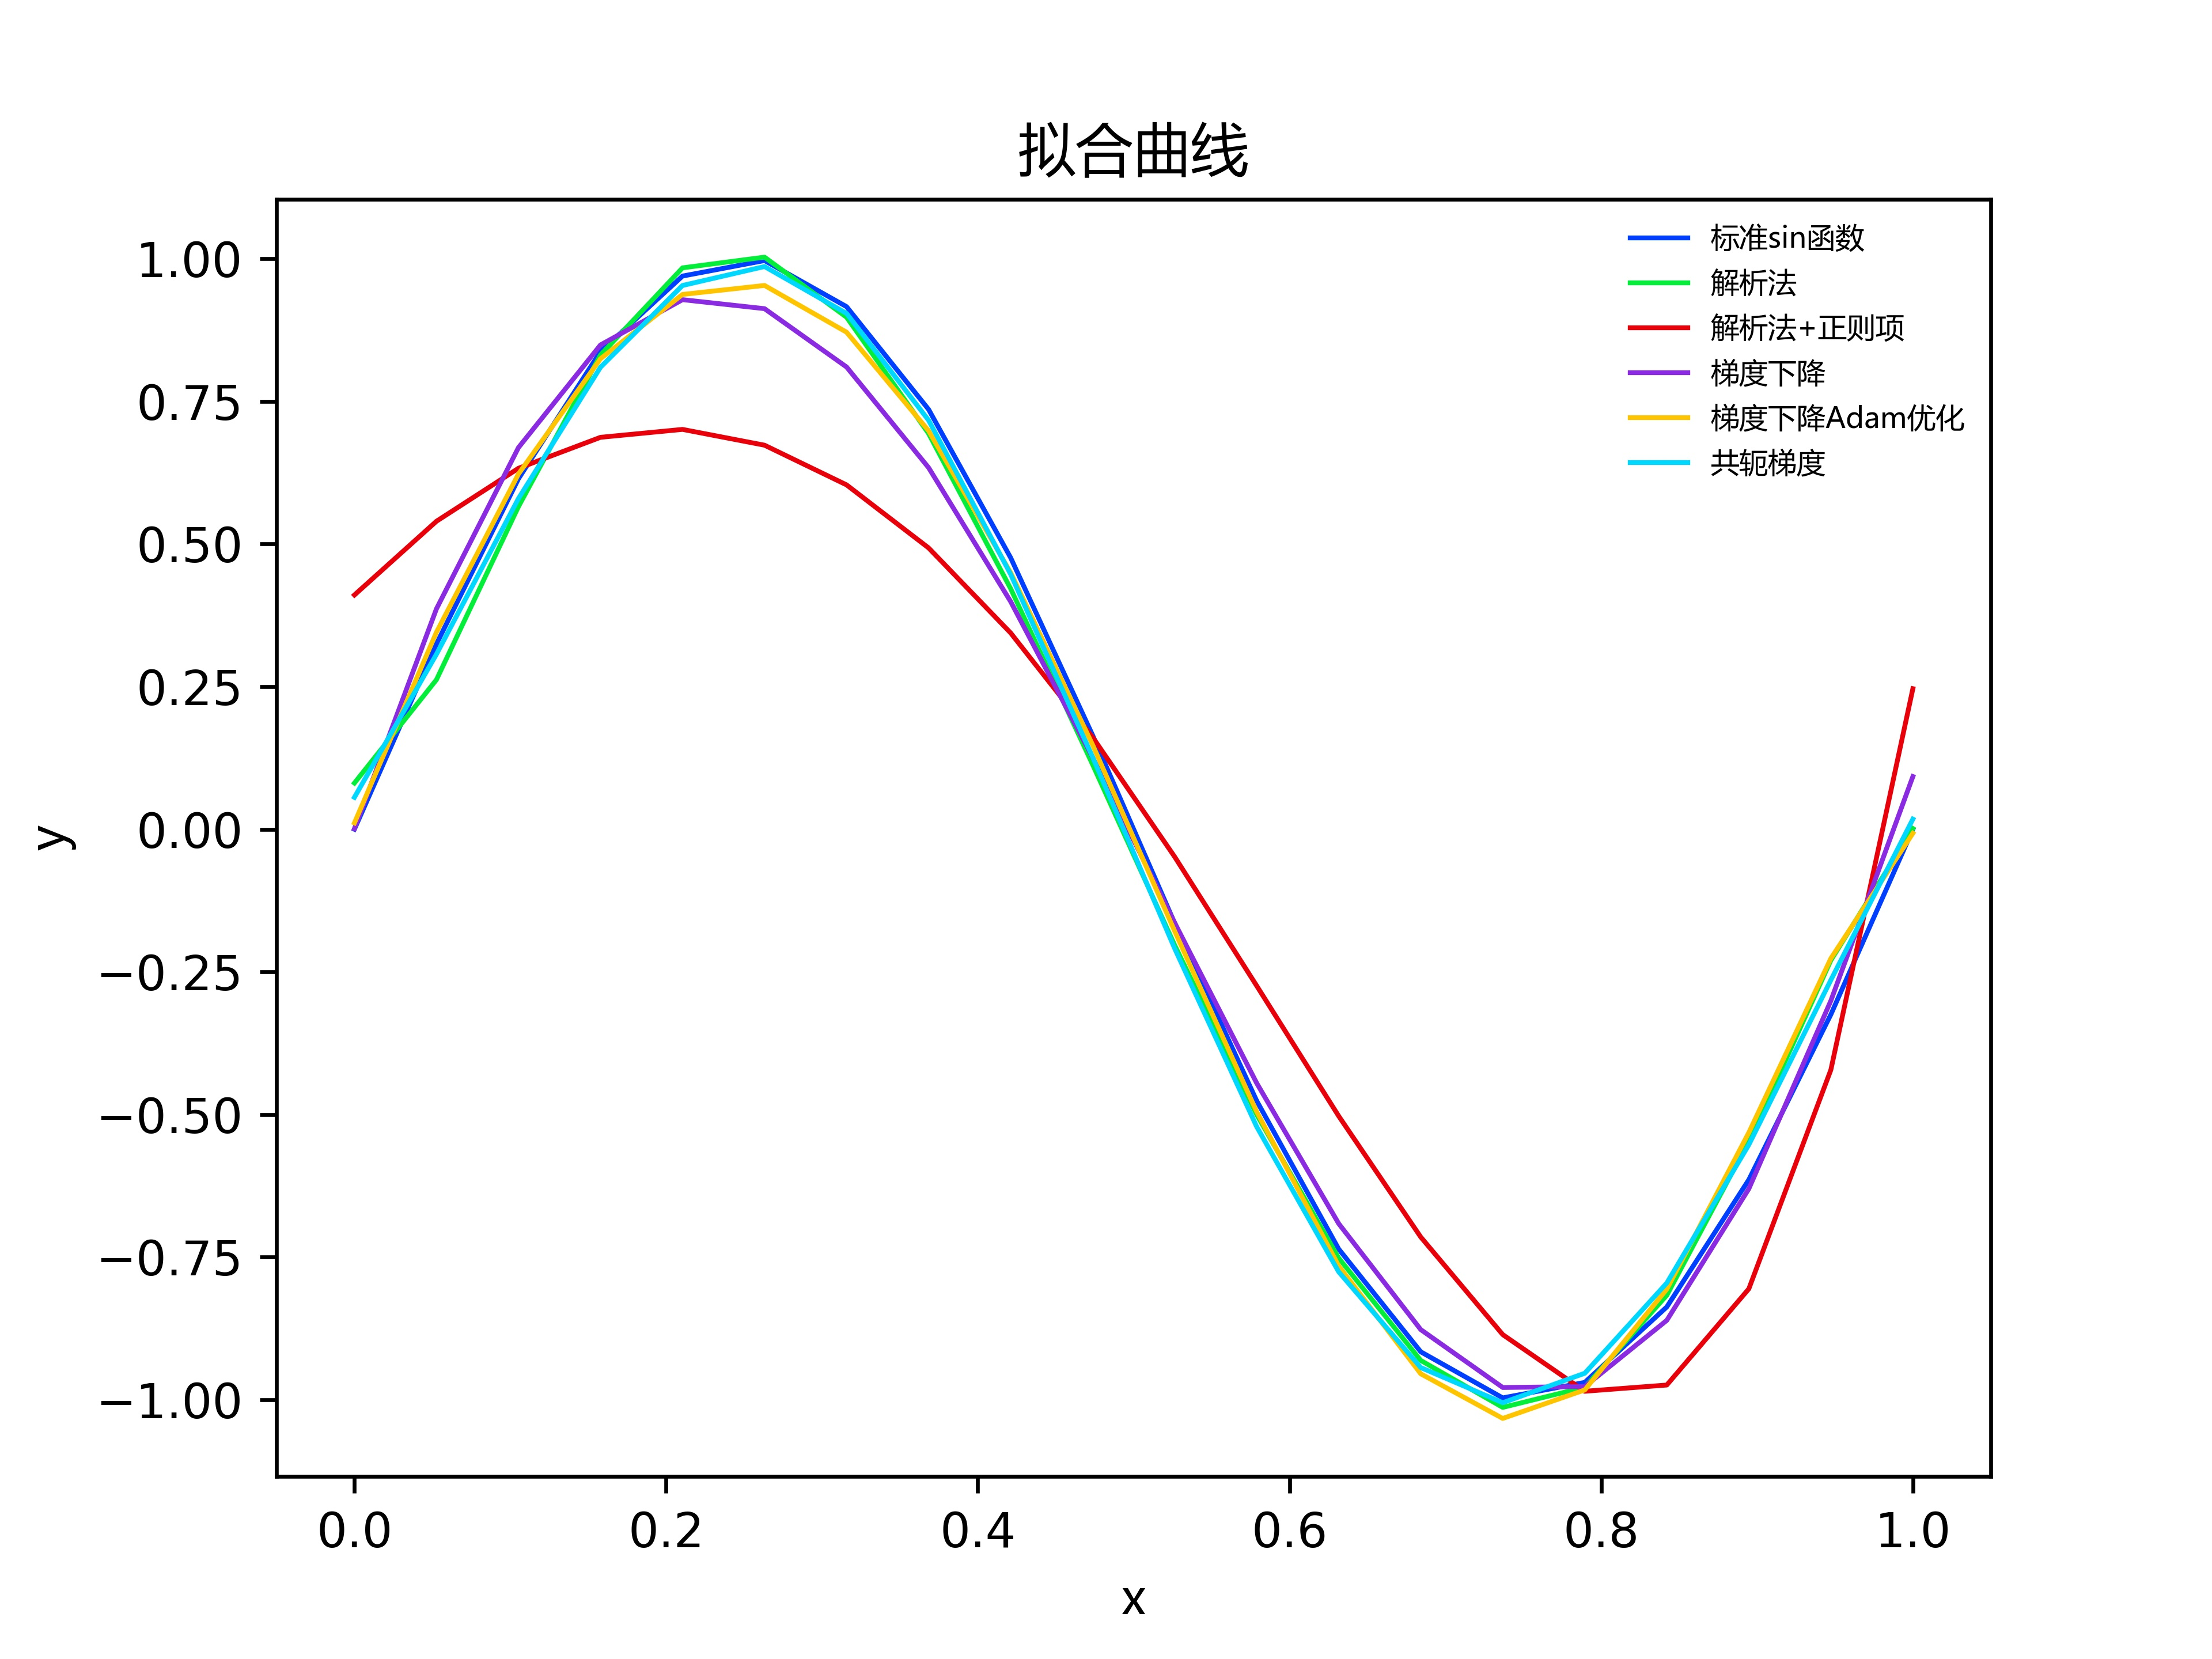
\includegraphics[width=0.3\textwidth]{n20o7}
}
\subfigure[8阶]{
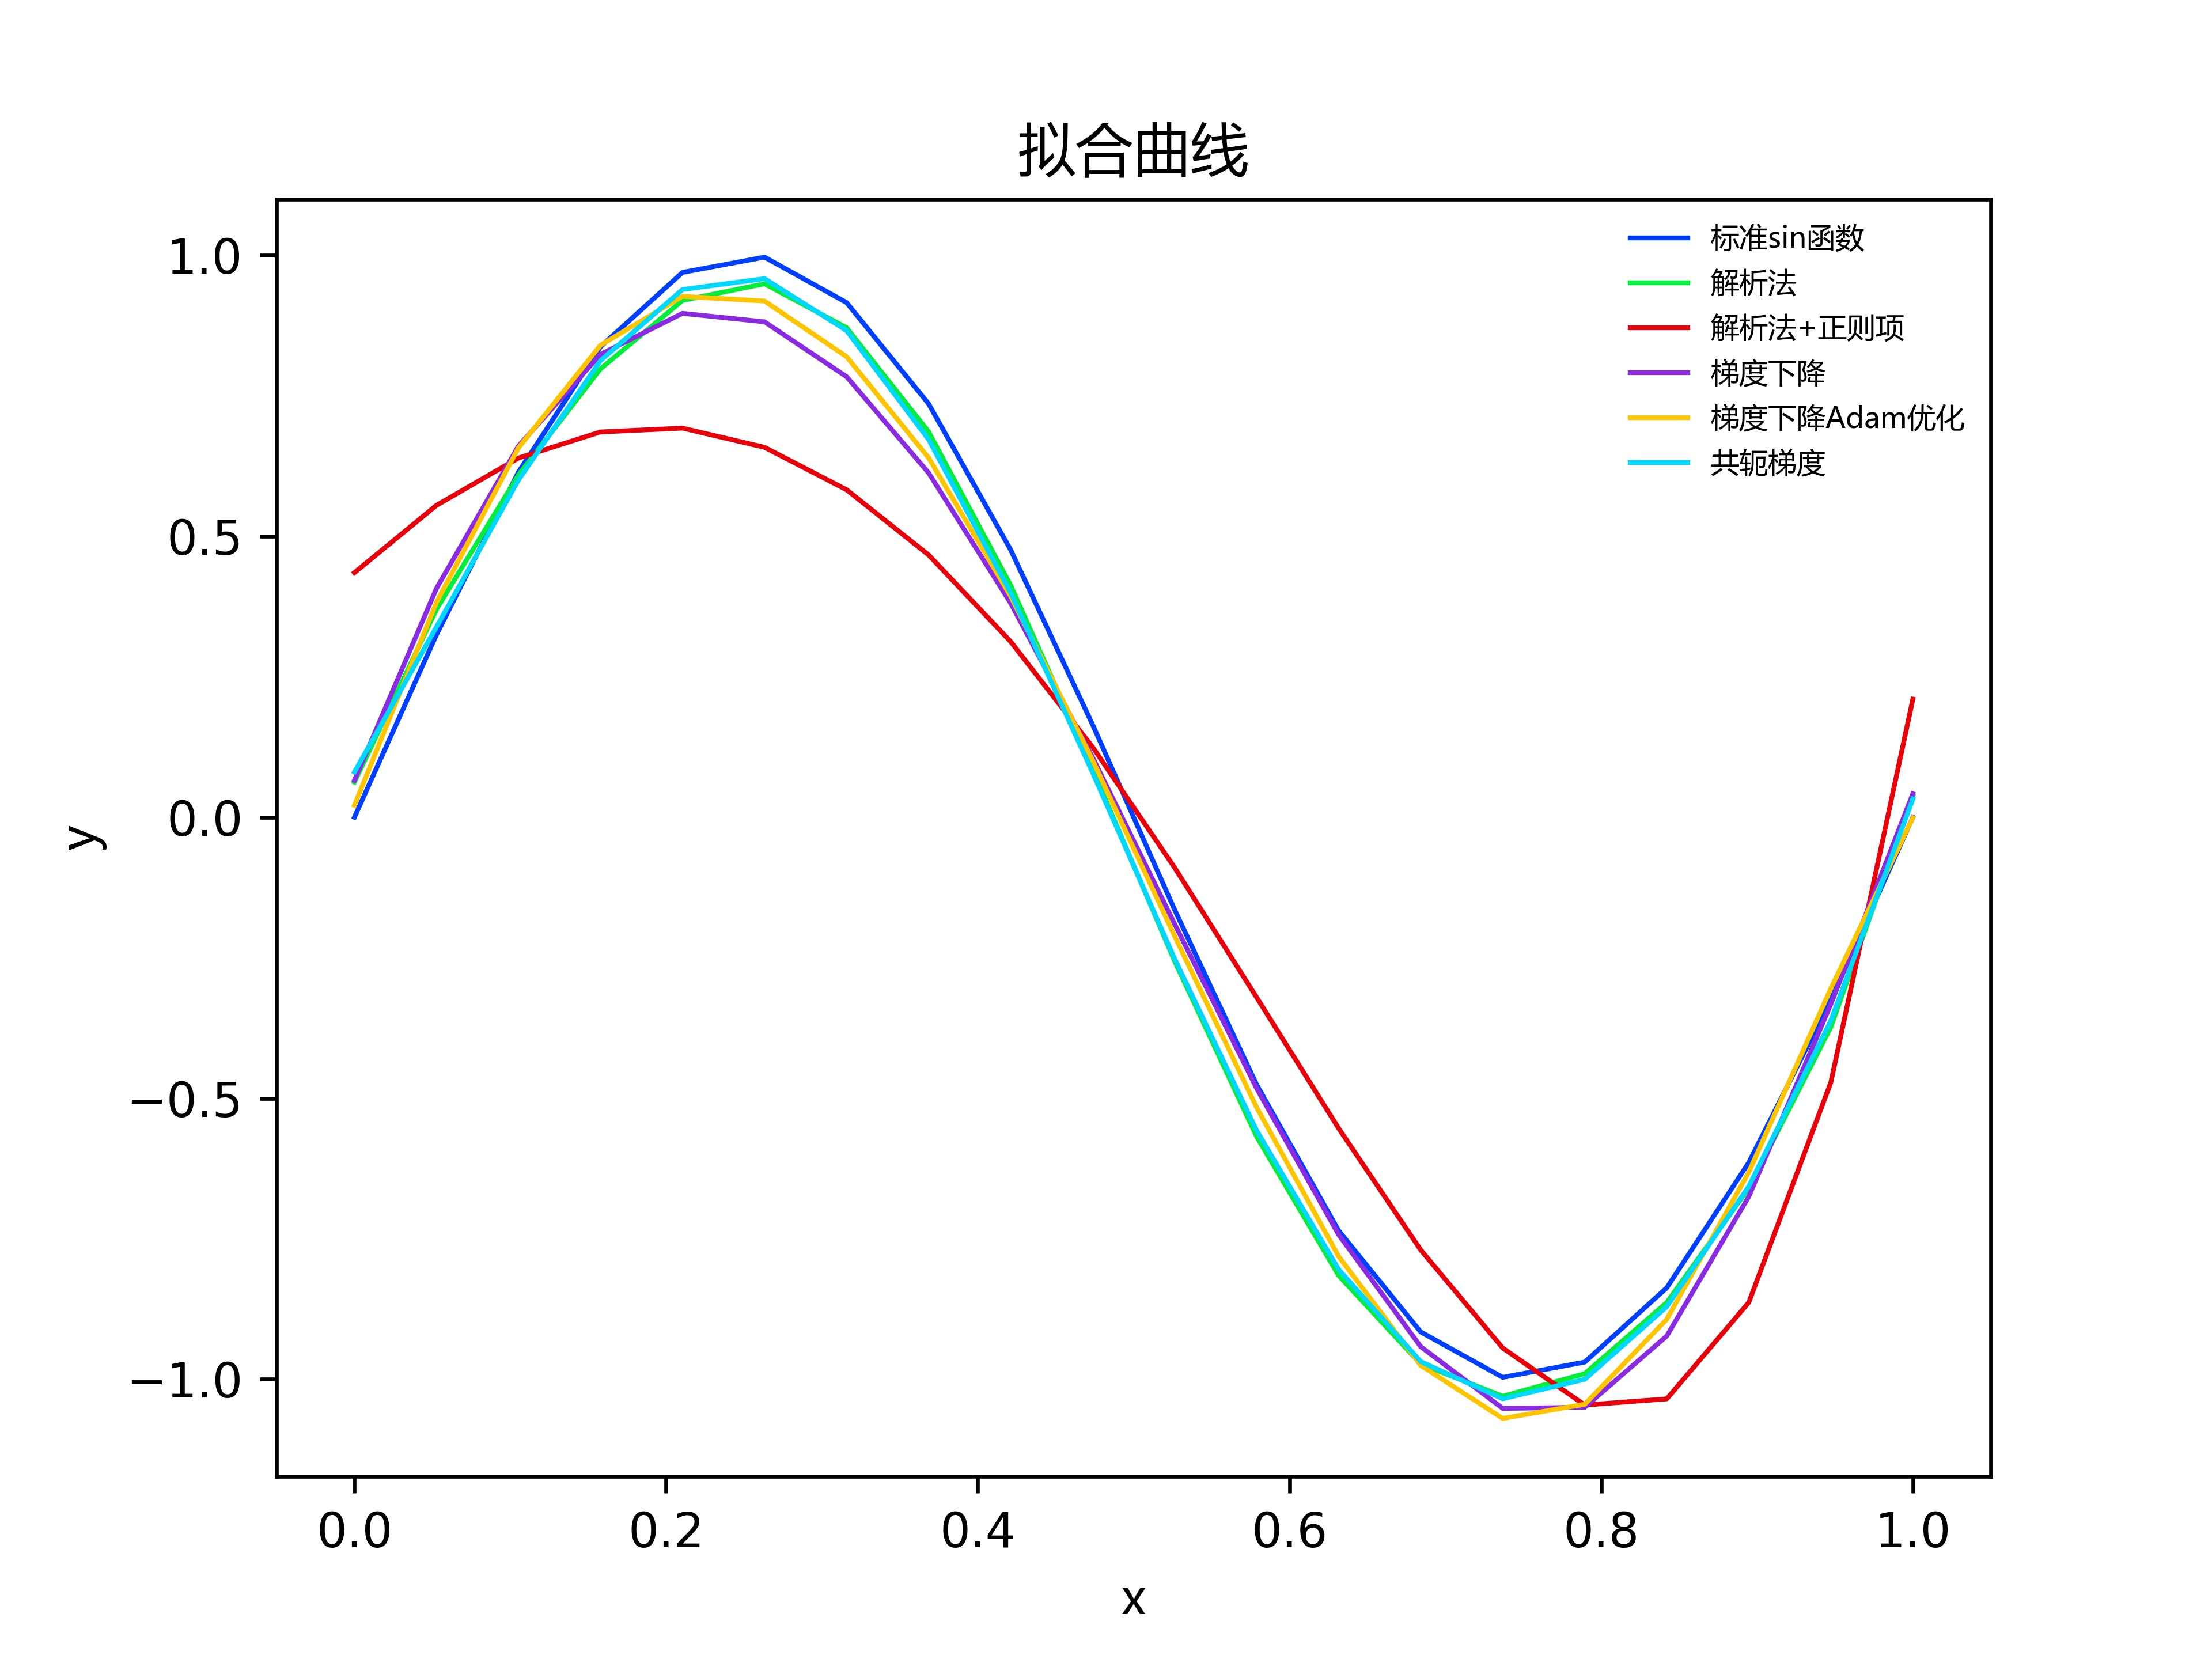
\includegraphics[width=0.3\textwidth]{n20o8}
}
\subfigure[9阶]{
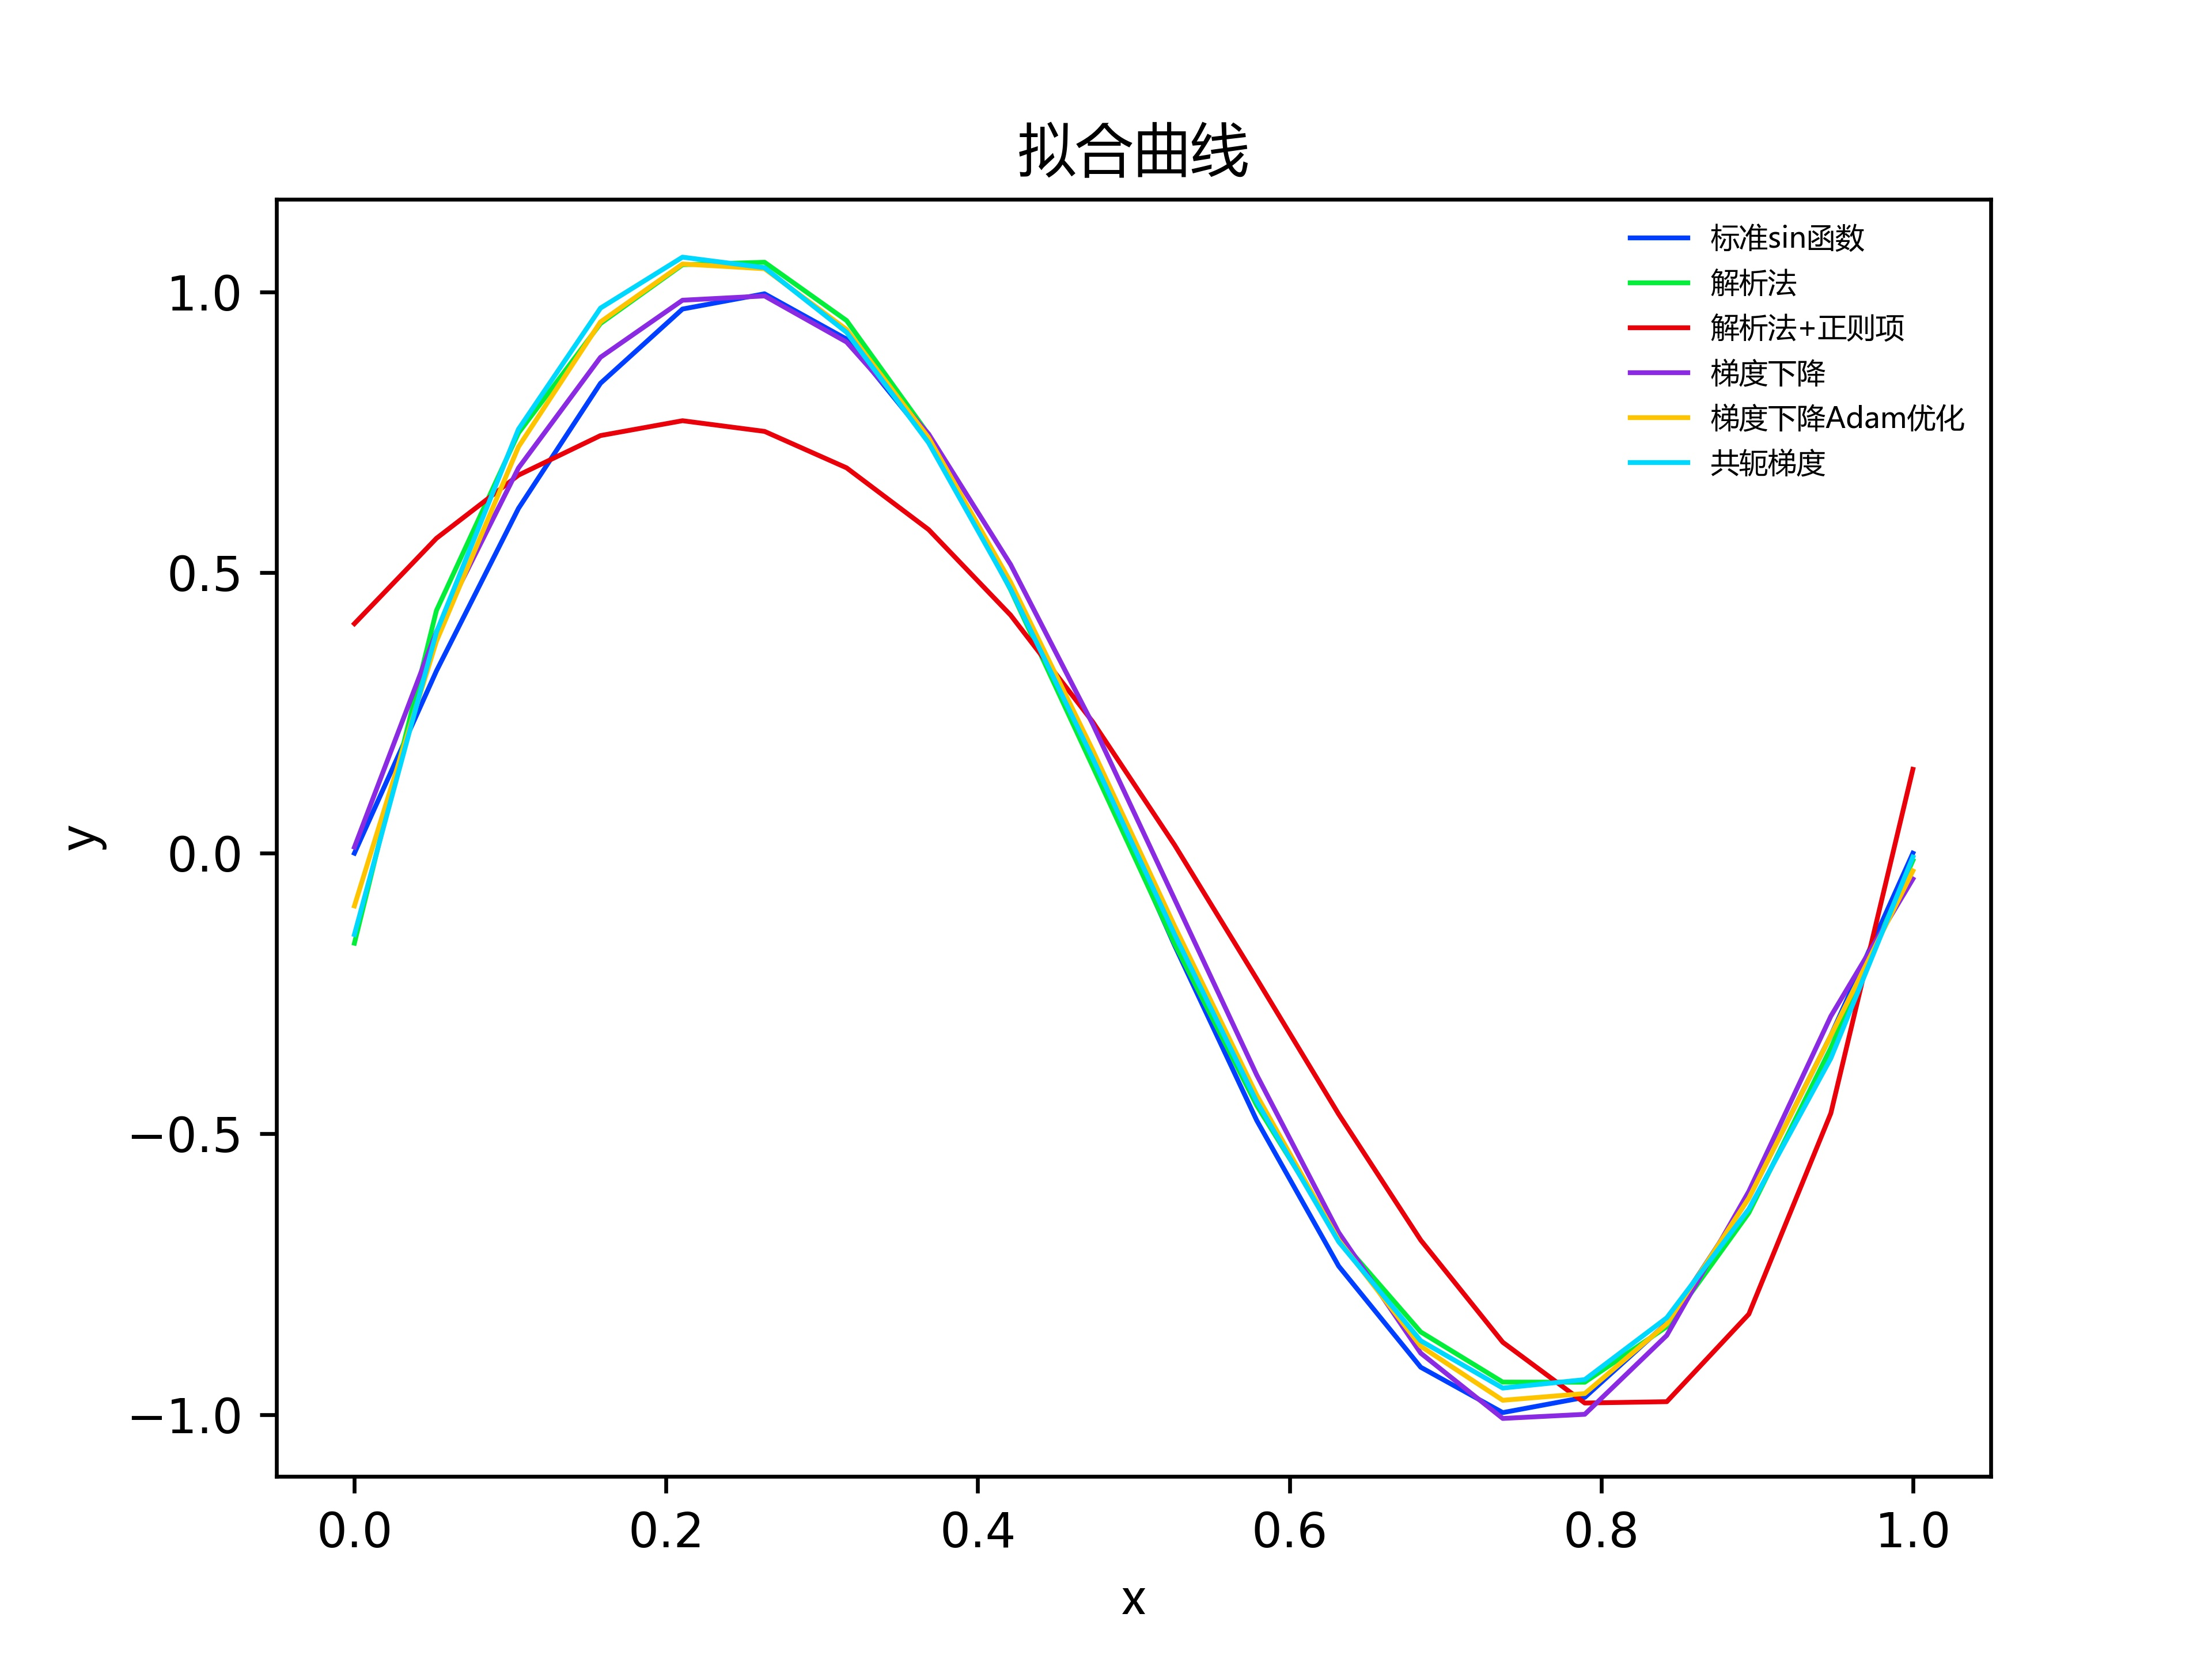
\includegraphics[width=0.3\textwidth]{n20o9}
}
\caption{n=20 不同阶拟合曲线}
\end{figure}

随着实验数据的增加,曲线更加光滑,但由于拟合优度也与数据集大小有关,因此拟合优度并无显著降低。拟合优度随阶数的变化趋势仍未变化。

\newpage
当数据集大小为50时,取多项式阶数为2,3,5,7,8,9。其拟合曲线及拟合优度如下。

\linespread{1.2}
\begin{table}[H]  
  \centering  
  \begin{threeparttable}  
  \caption{n=50 不同阶拟合优度}  
  \label{tab:performance_comparison} 
  \begin{tabular}{m{0.1\textwidth}<{\centering} m{0.15\textwidth}<{\centering} m{0.15\textwidth}<{\centering} m{0.15\textwidth}<{\centering} m{0.15\textwidth}<{\centering} m{0.15\textwidth}<{\centering}}  
    \toprule[1.5pt]  
    \multirow{2}{*}{阶数}&\multicolumn{2}{c}{解析法}&\multicolumn{2}{c}{梯度下降} &\multirow{2}{*}{共轭梯度}\cr  
    \cmidrule(lr){2-3} \cmidrule(lr){4-5}  
    &不含正则项&含正则项&未优化&优化后\cr  
    \midrule  
2&0.6497&0.6498&0.6498&0.6497&0.6497\cr
3&0.1141&0.3675&0.1246&0.1141&0.1141\cr
5&0.0339&0.2087&0.1455&0.0675&0.0339\cr
7&0.0799&0.2444&0.1125&0.0802&0.0782\cr
8&0.0503&0.2136&0.0670&0.0543&0.0490\cr
9&0.0762&0.1953&0.0654&0.0568&0.0688\cr
    \bottomrule  
    \end{tabular}  
    \end{threeparttable}  
\end{table}

\begin{figure}[H]
\centering
\subfigure[2阶]{
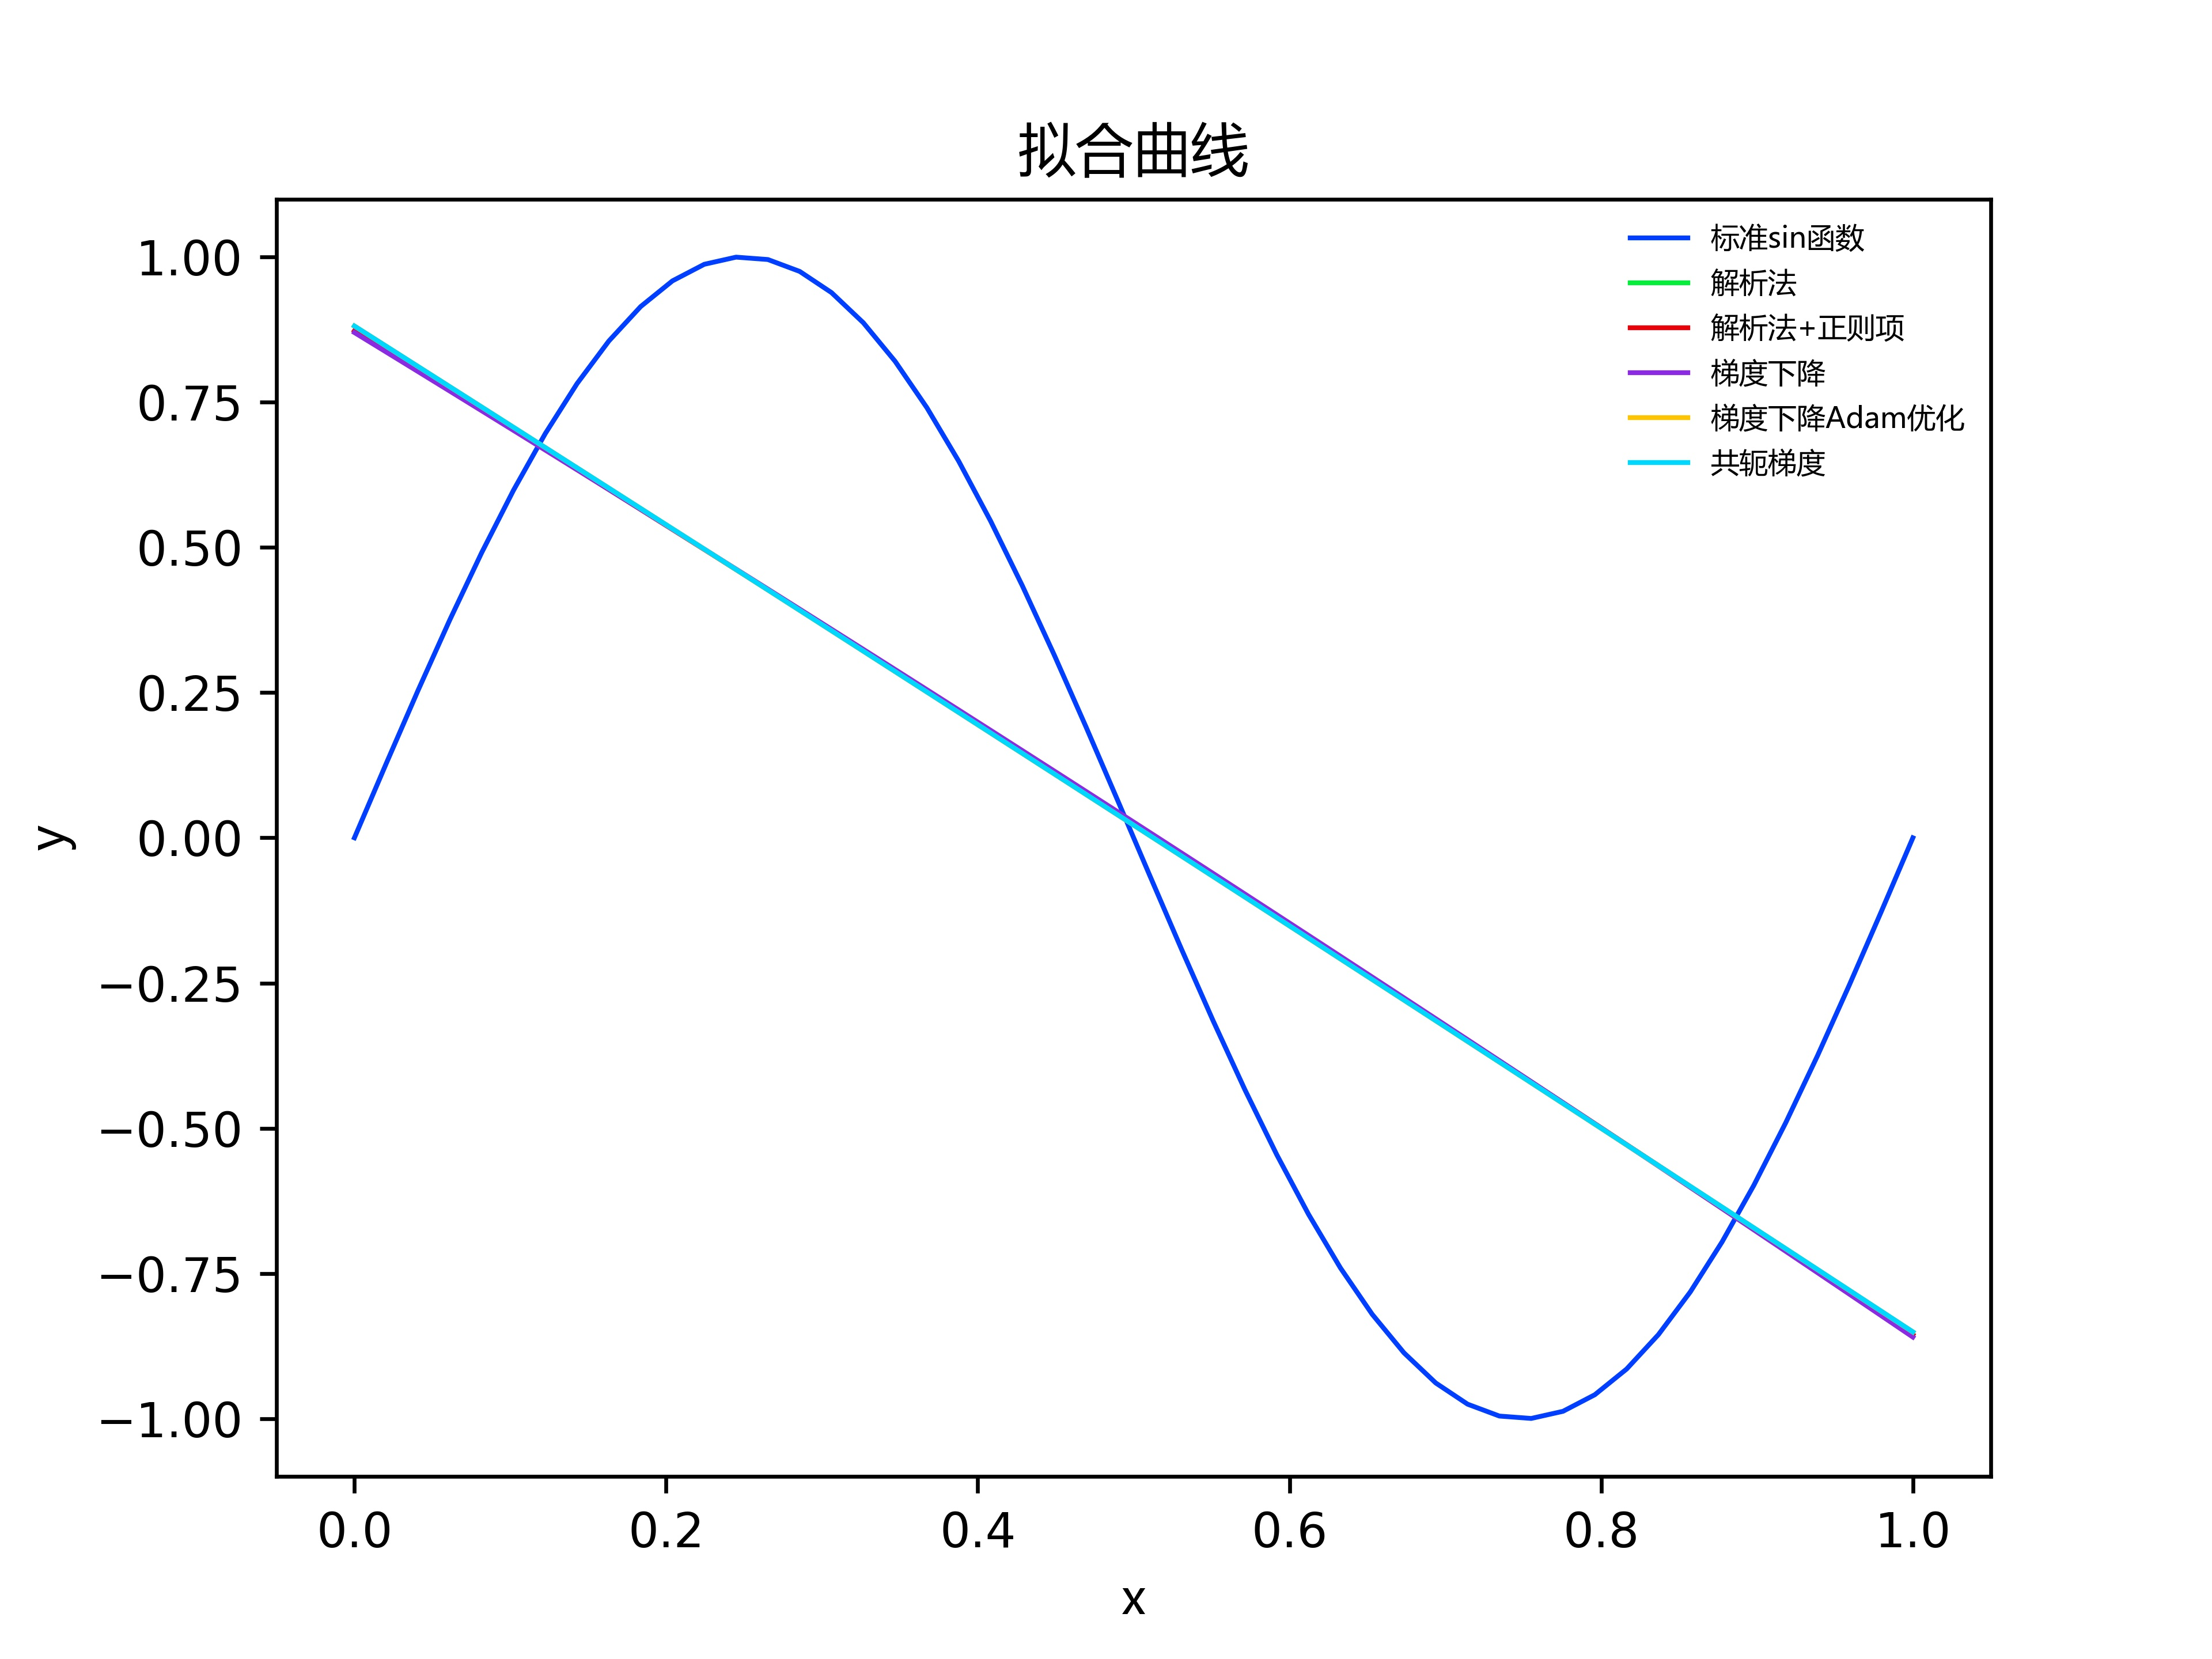
\includegraphics[width=0.3\textwidth]{n50o2}
}
\subfigure[3阶]{
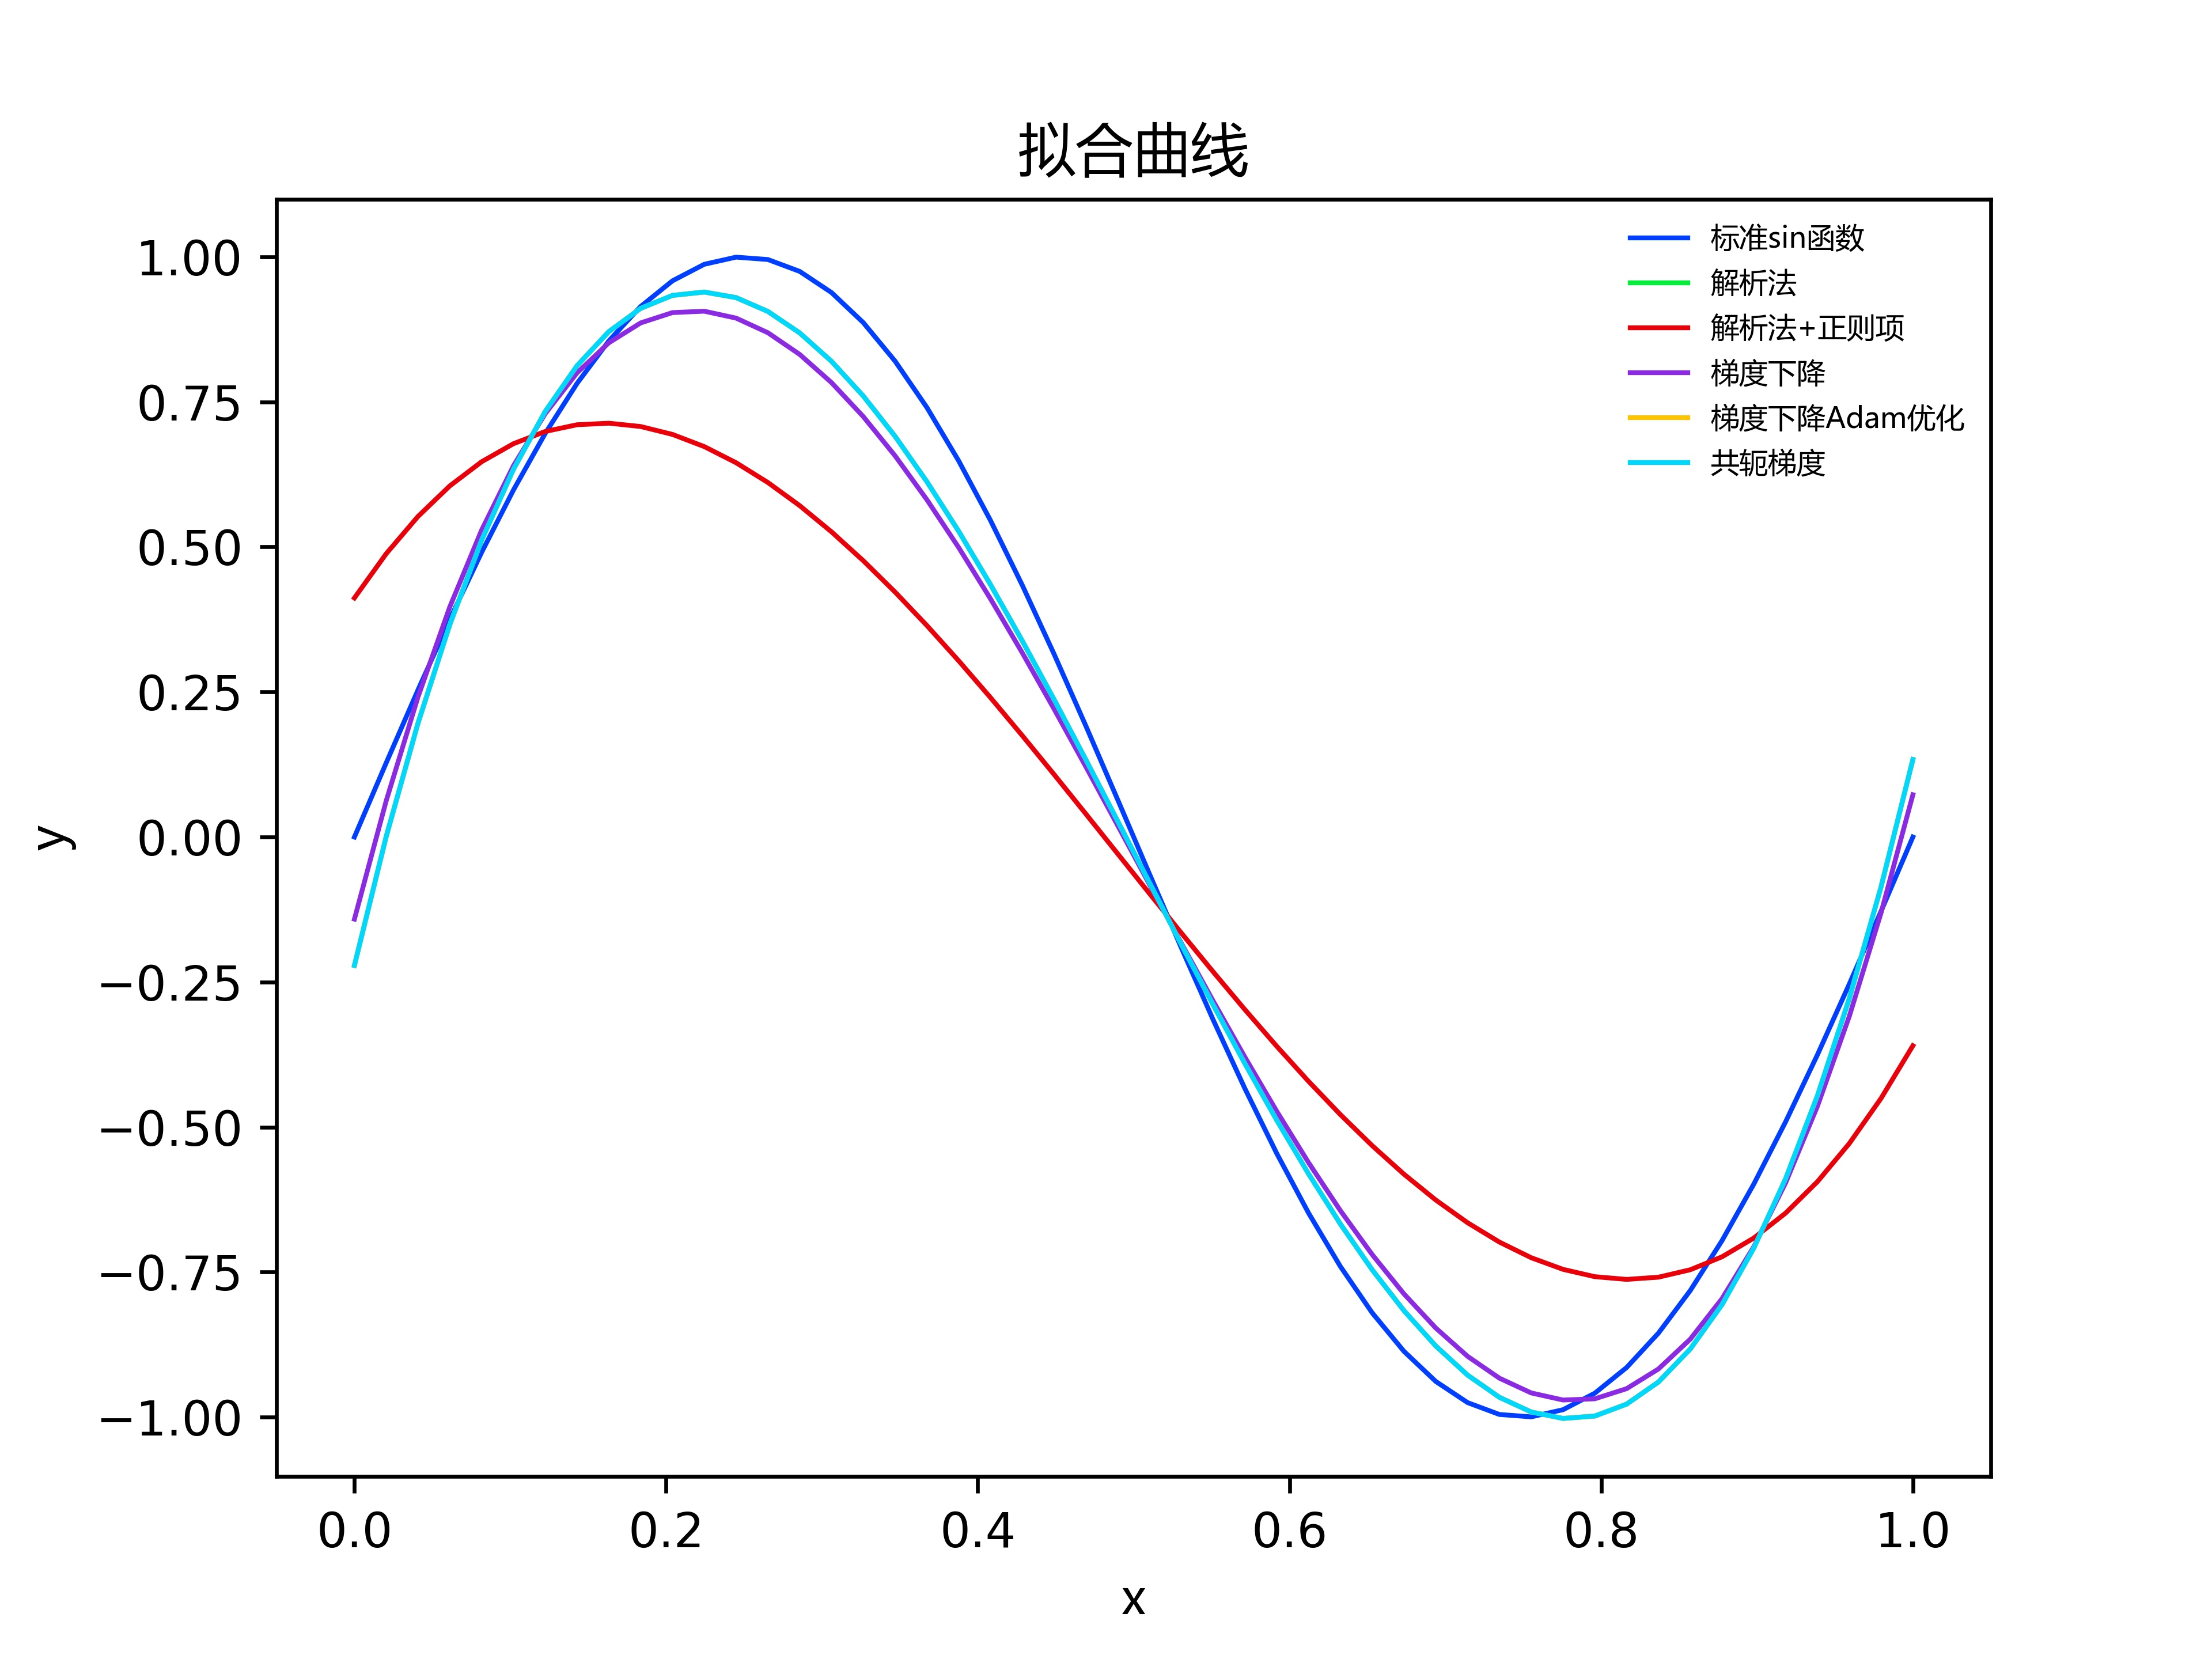
\includegraphics[width=0.3\textwidth]{n50o3}
}
\subfigure[5阶]{
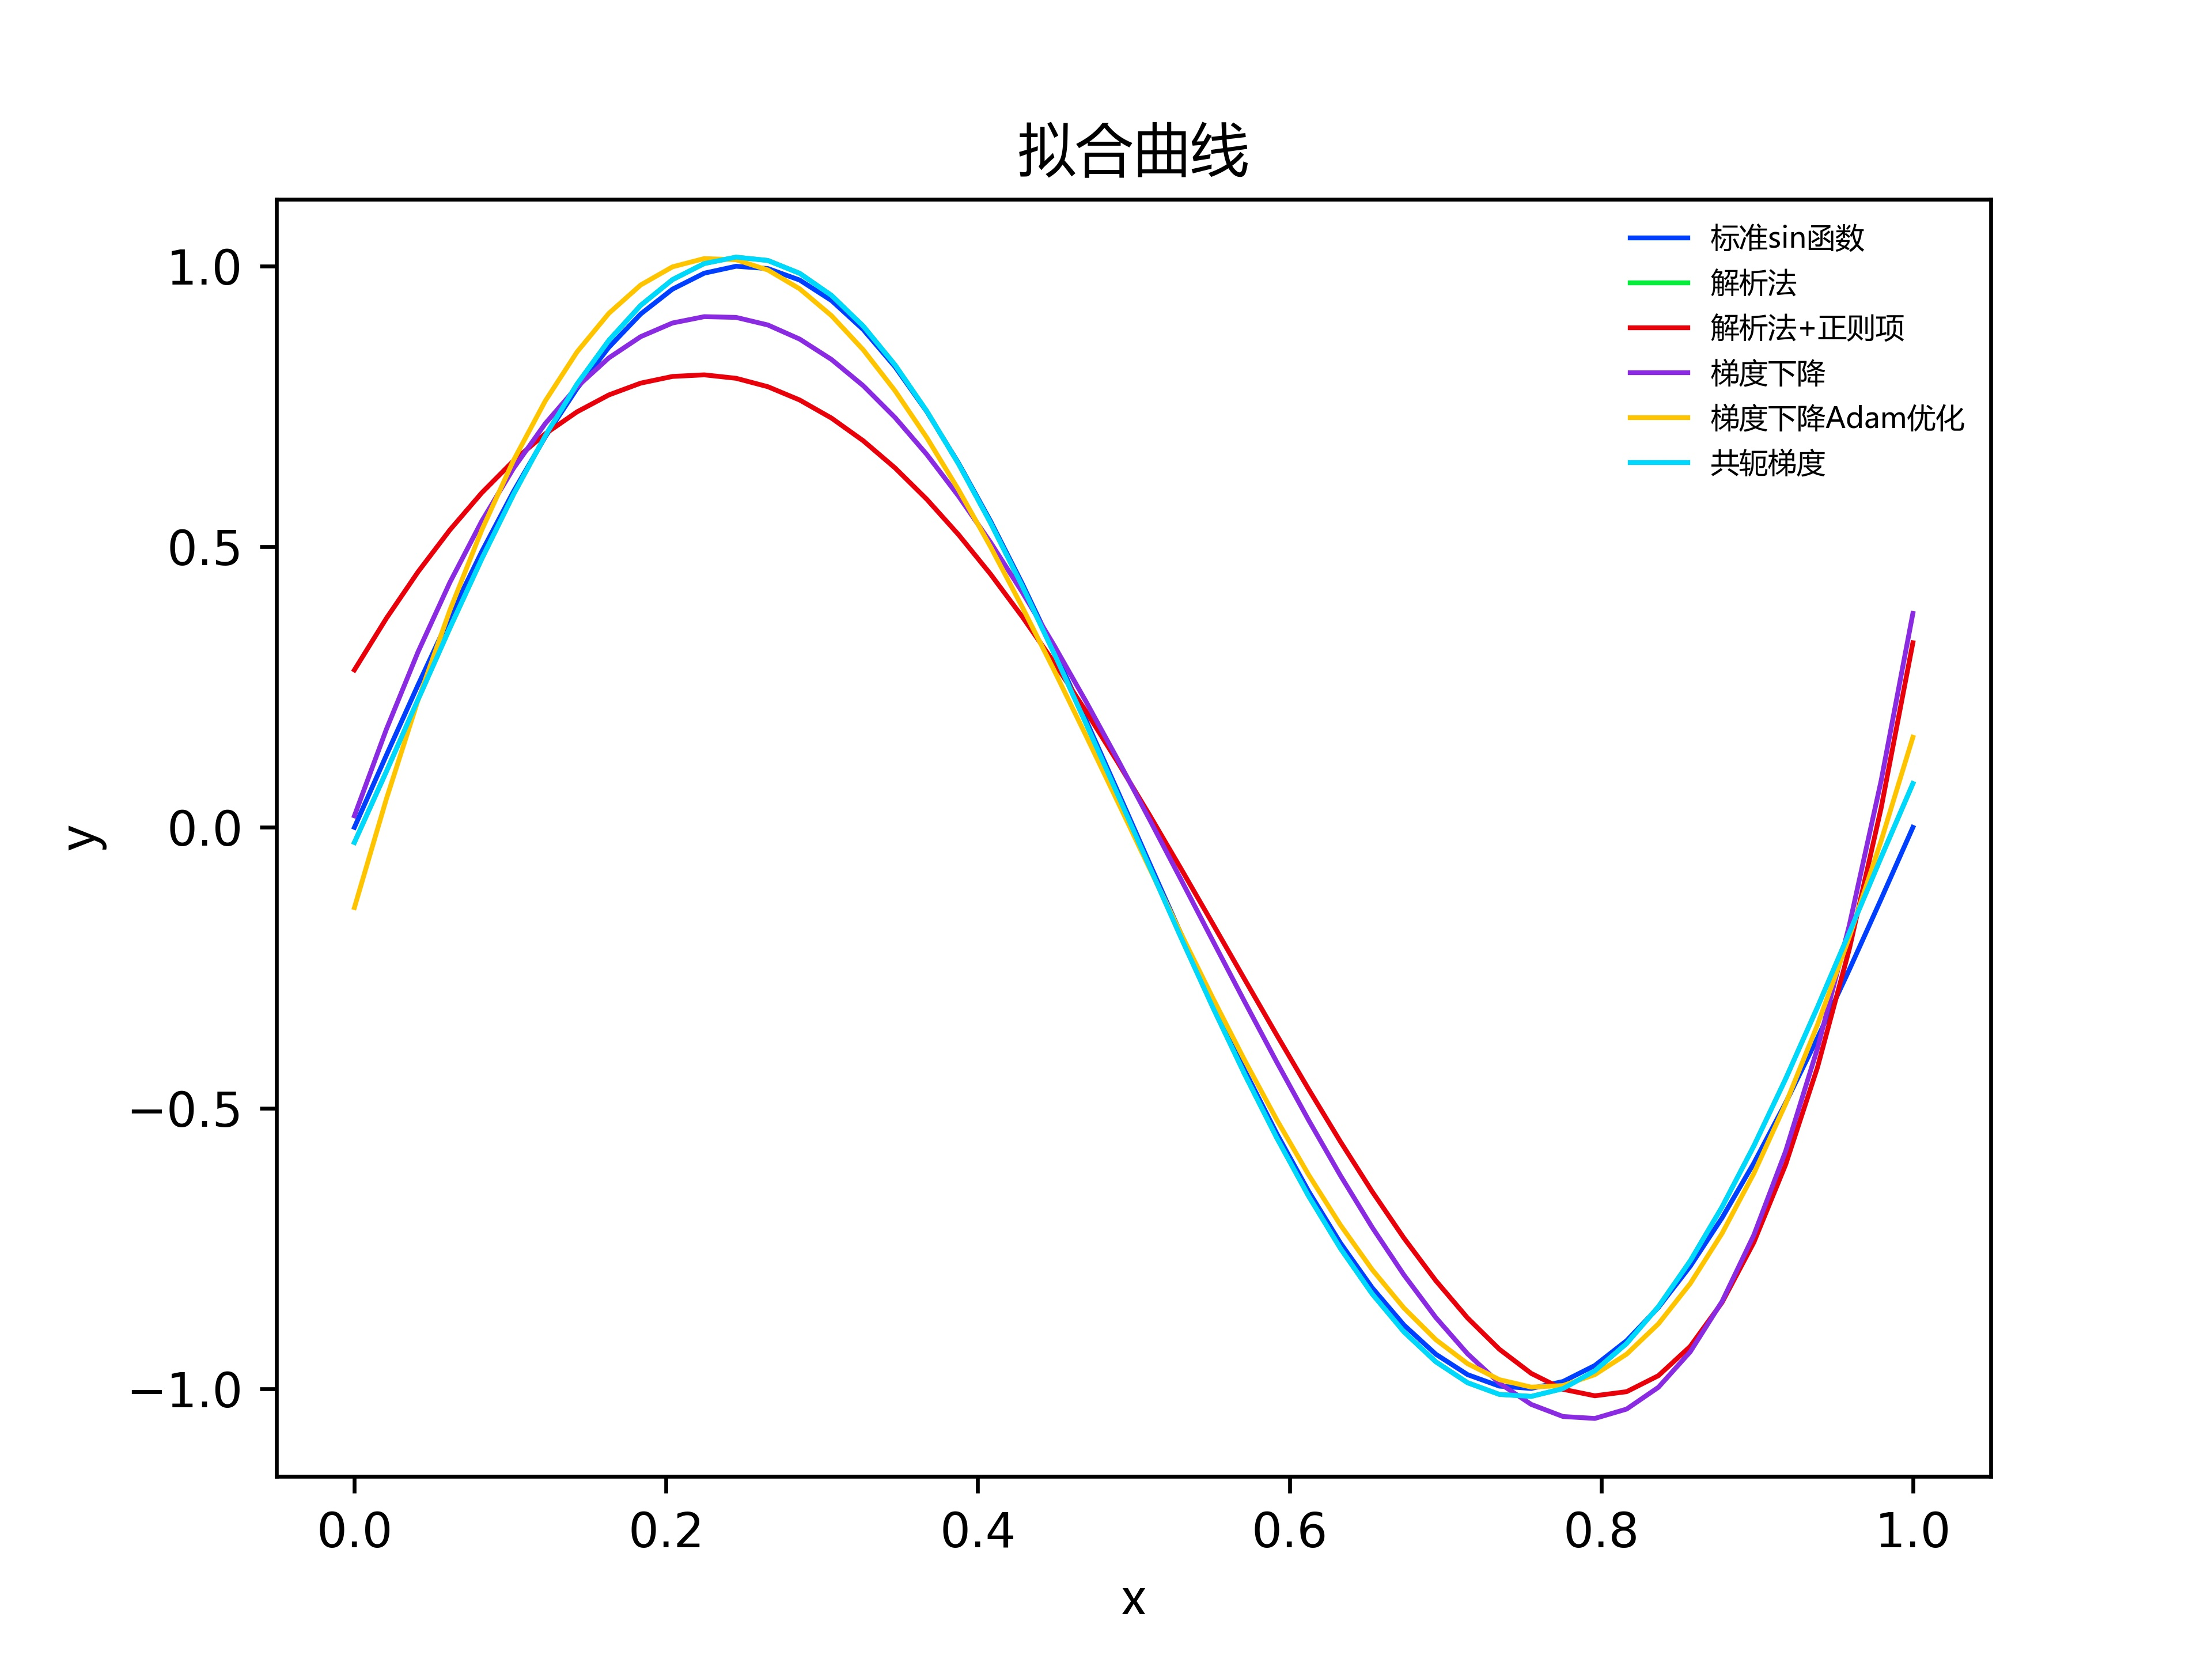
\includegraphics[width=0.3\textwidth]{n50o5}
}
\quad
\subfigure[7阶]{
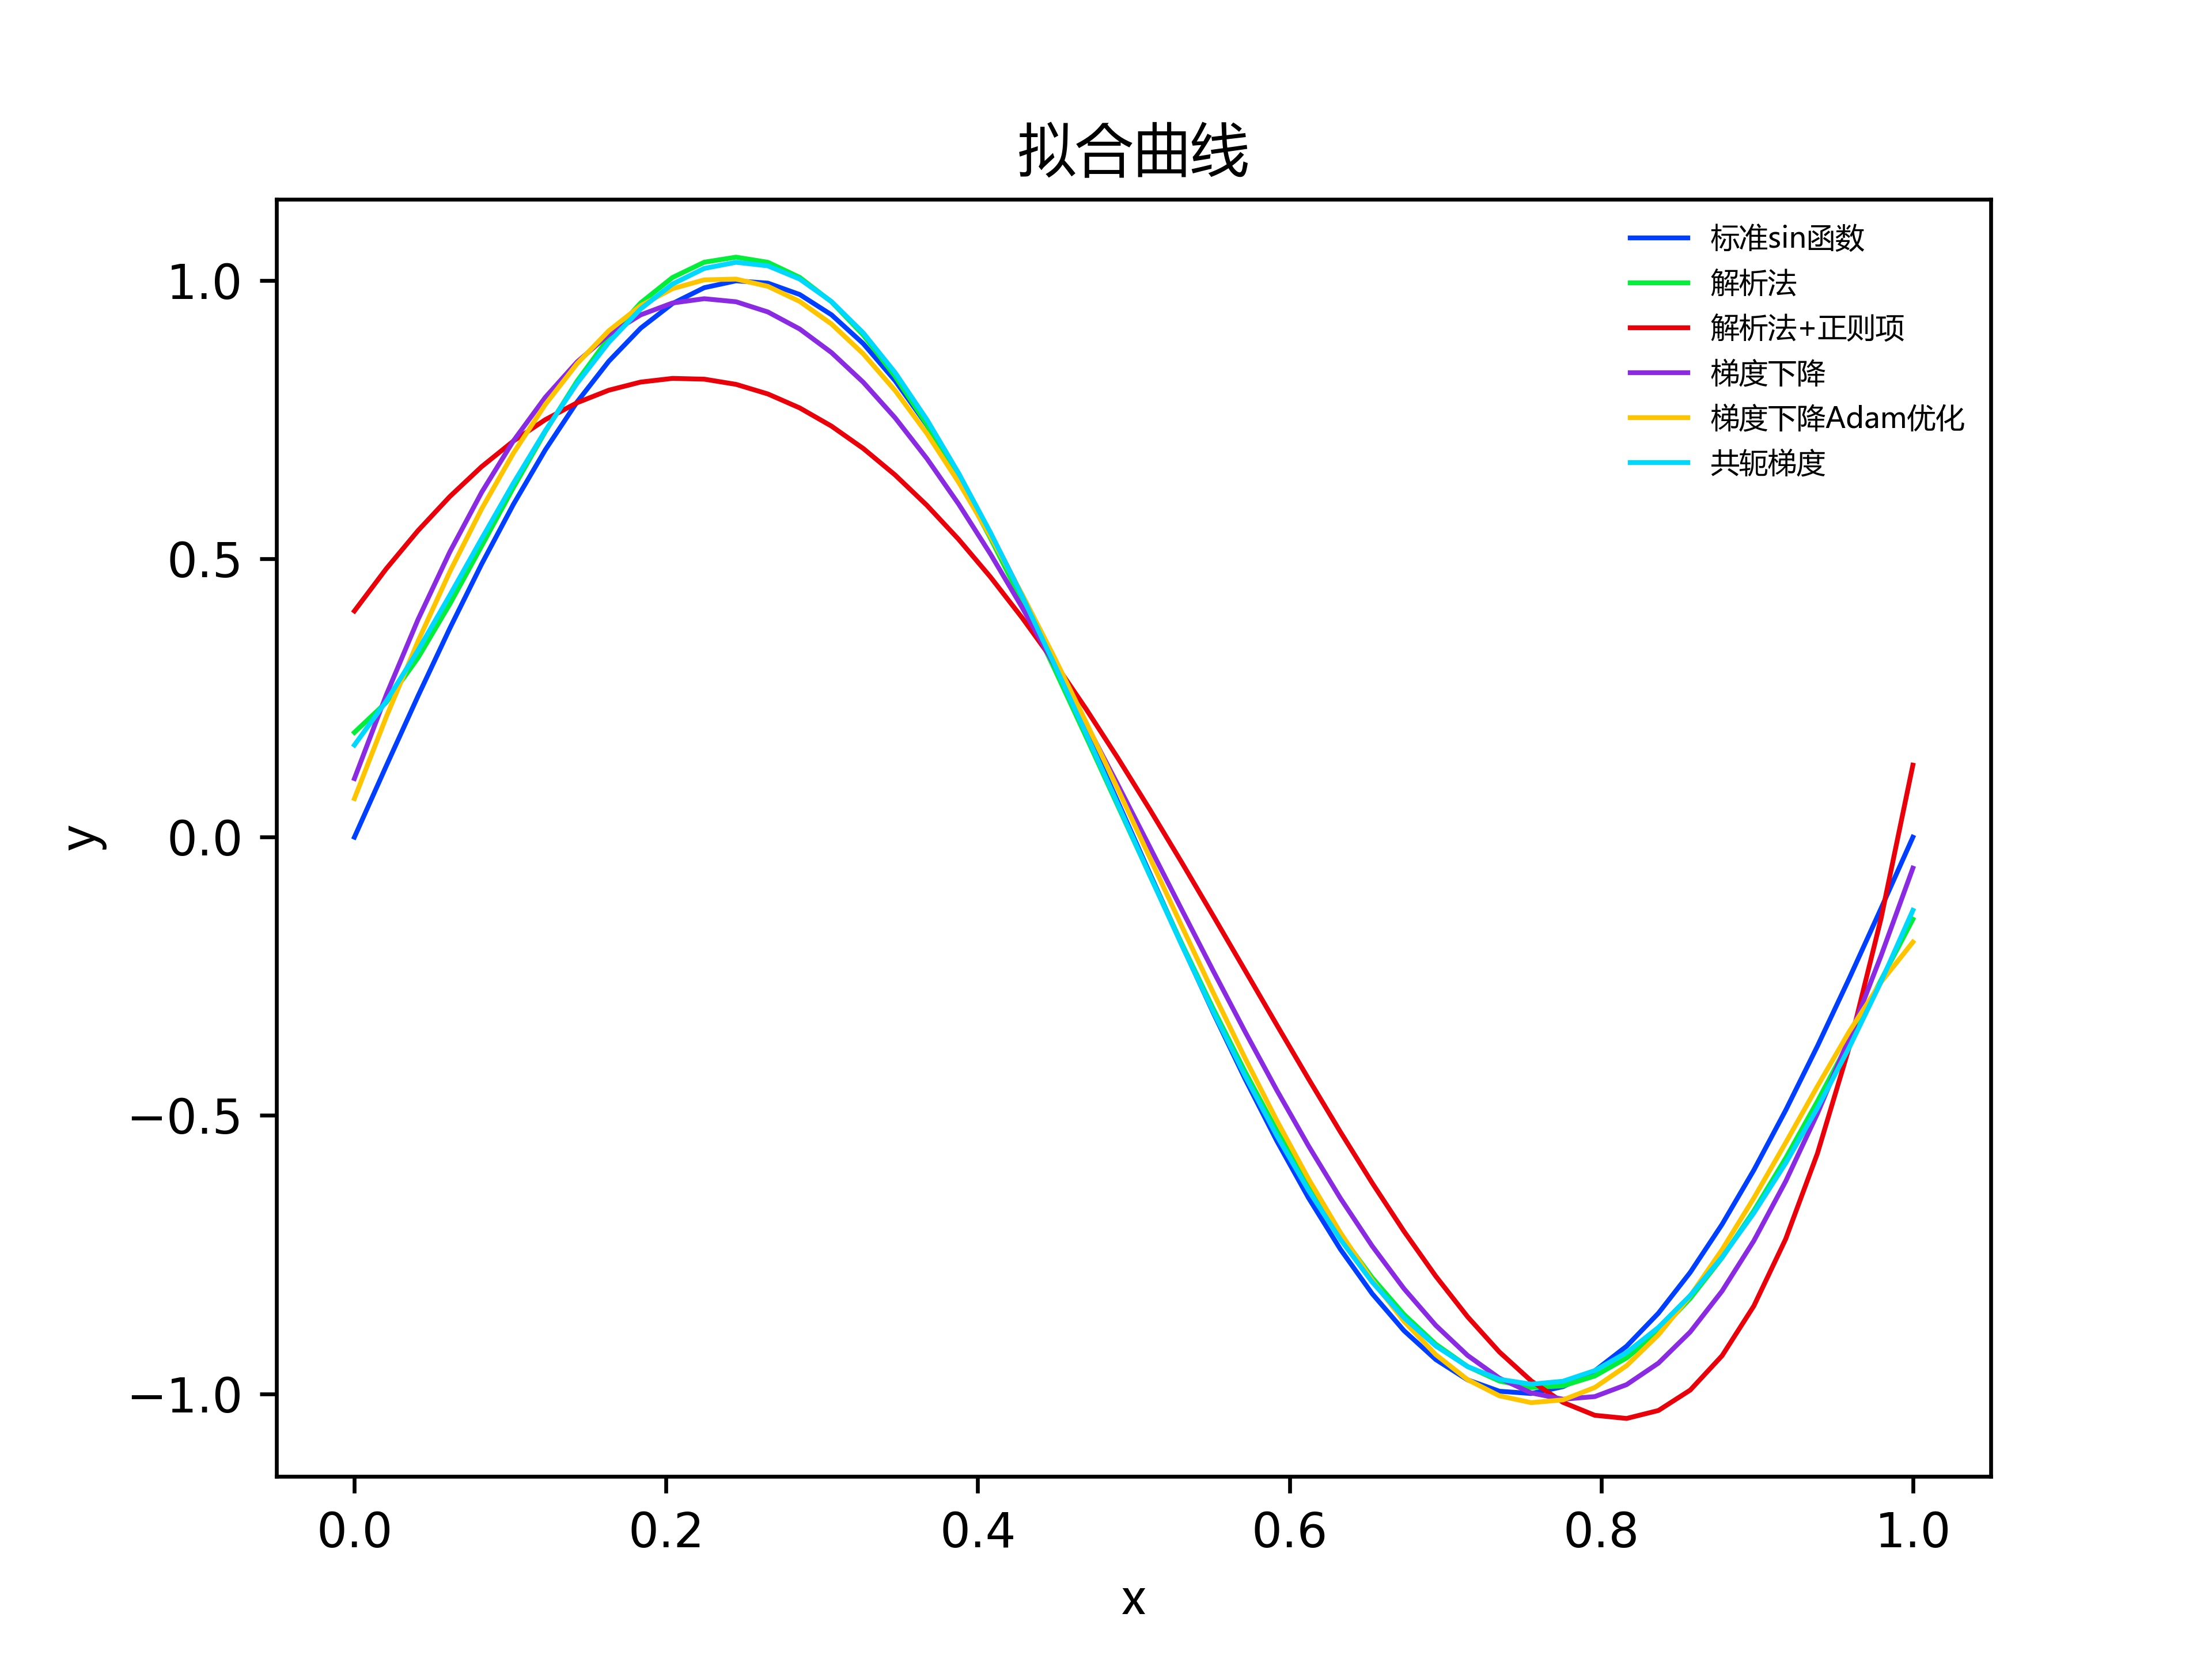
\includegraphics[width=0.3\textwidth]{n50o7}
}
\subfigure[8阶]{
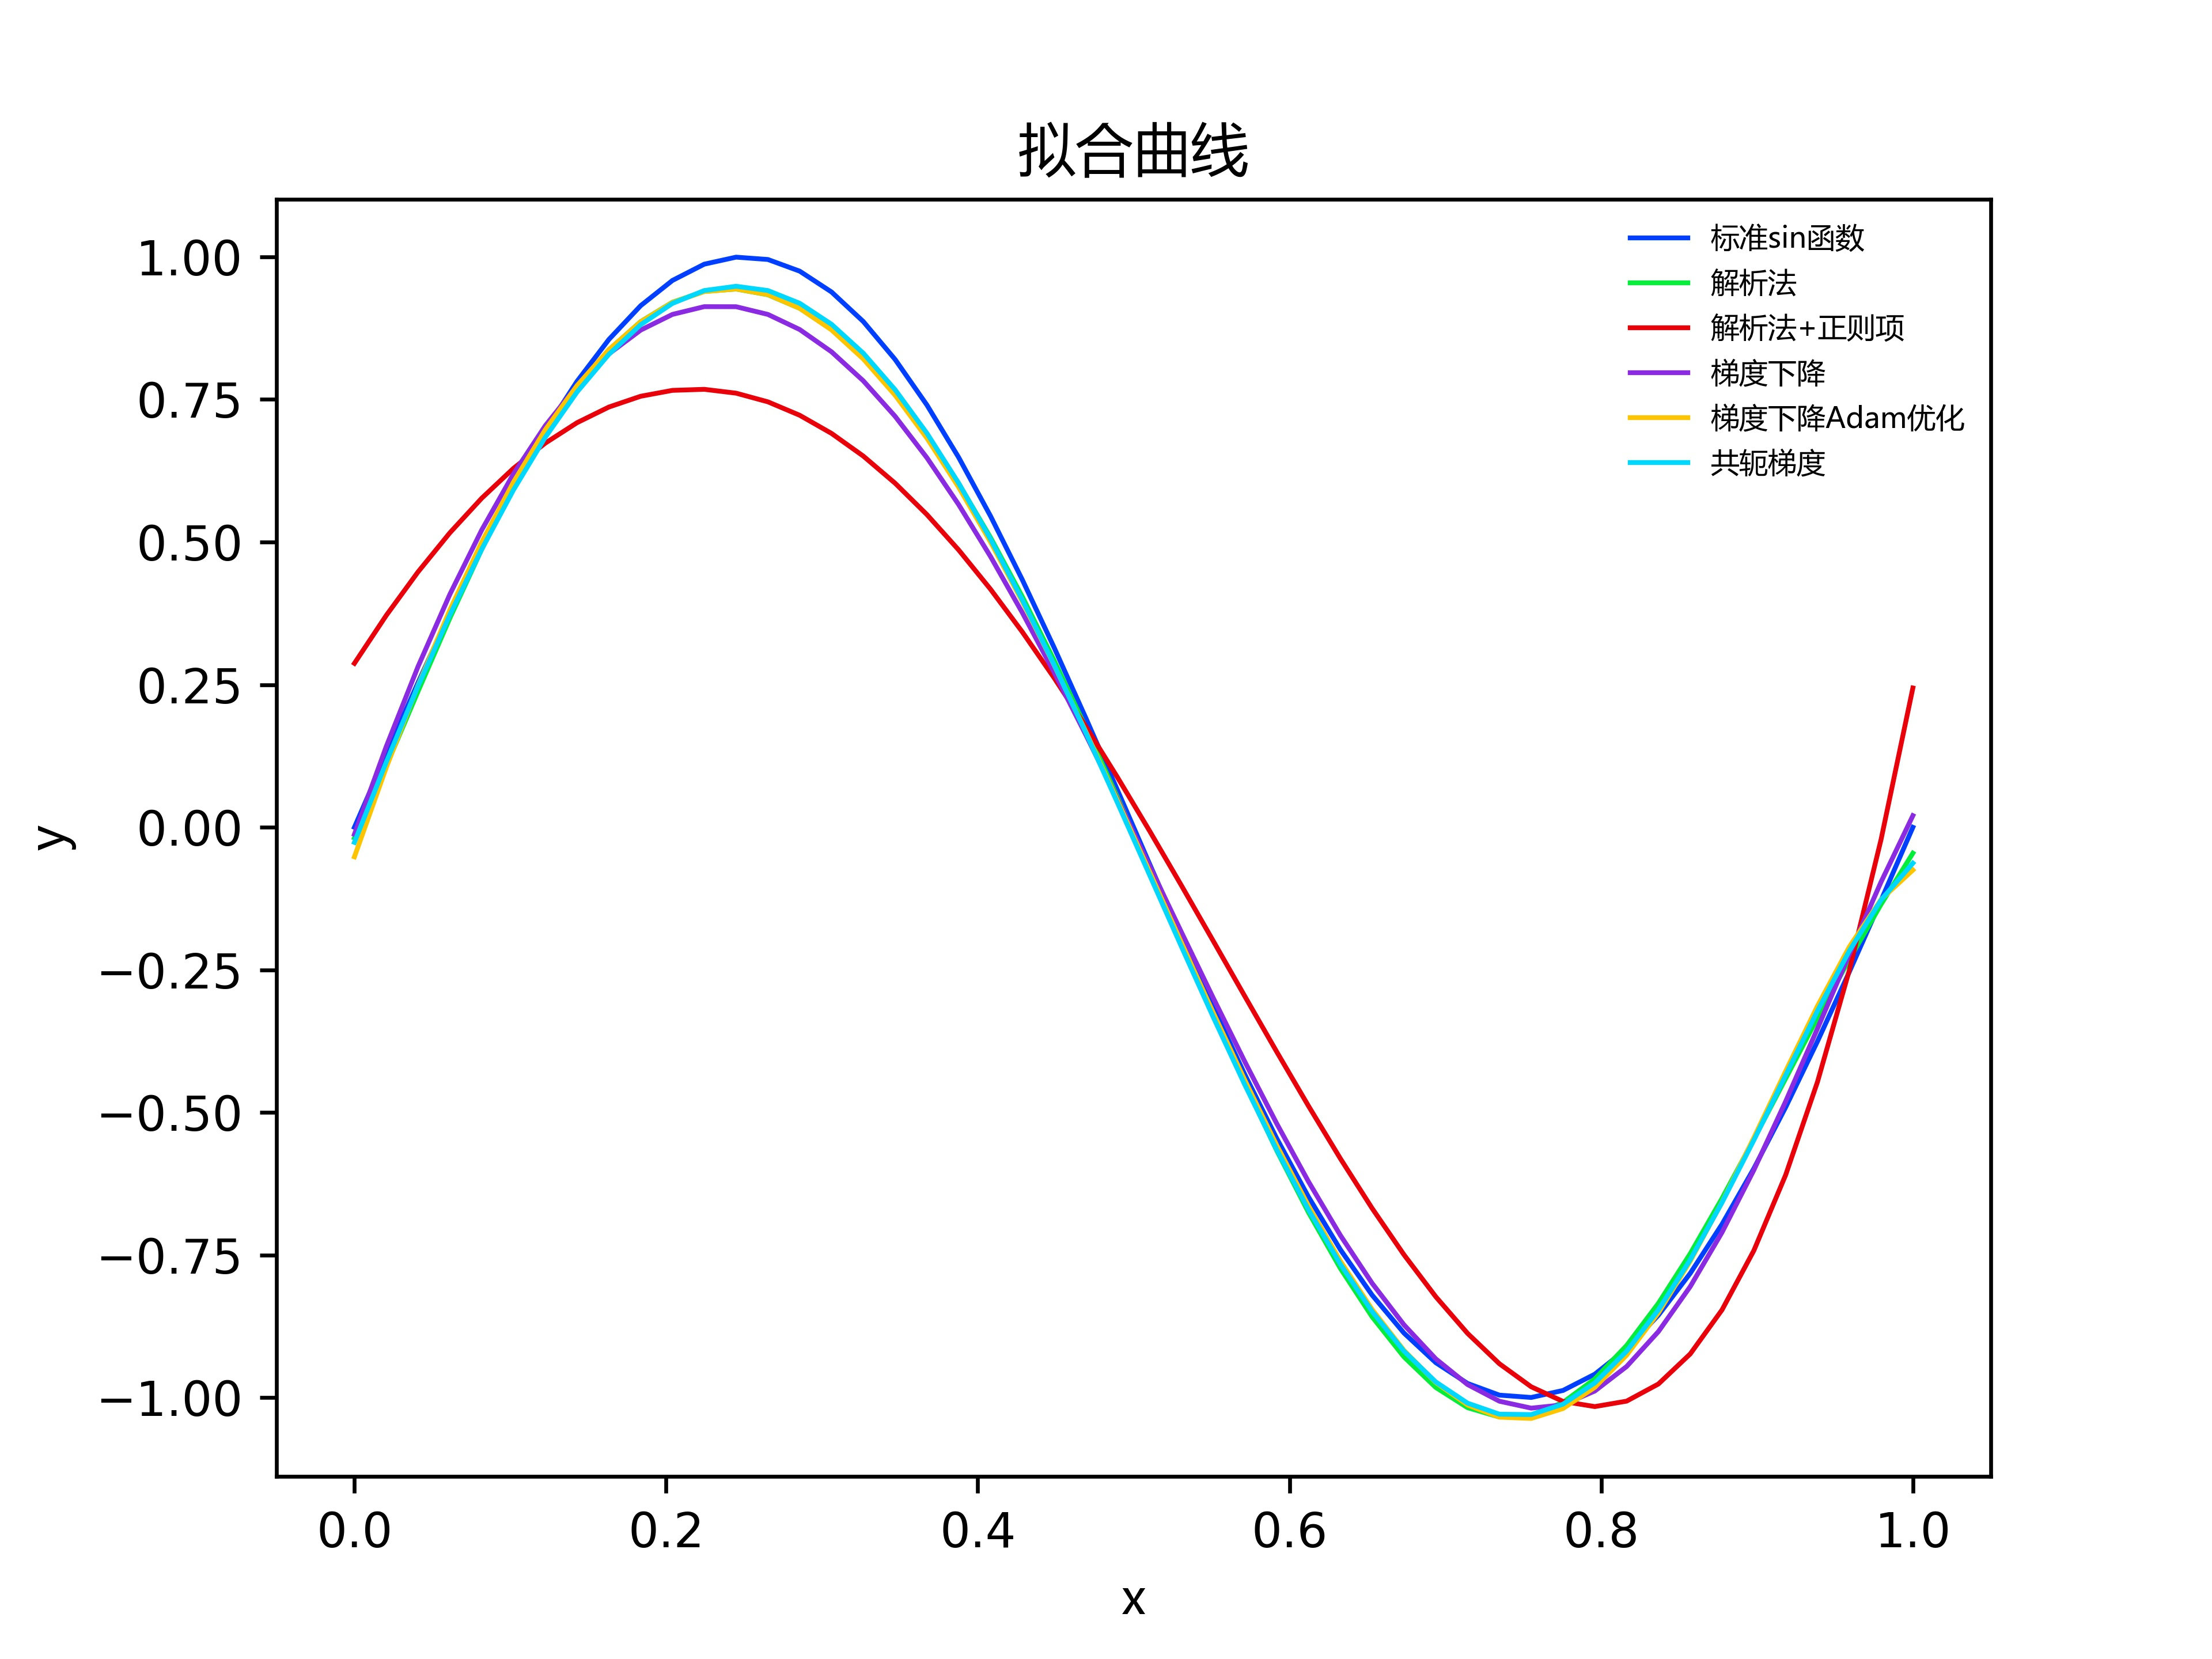
\includegraphics[width=0.3\textwidth]{n50o8}
}
\subfigure[9阶]{
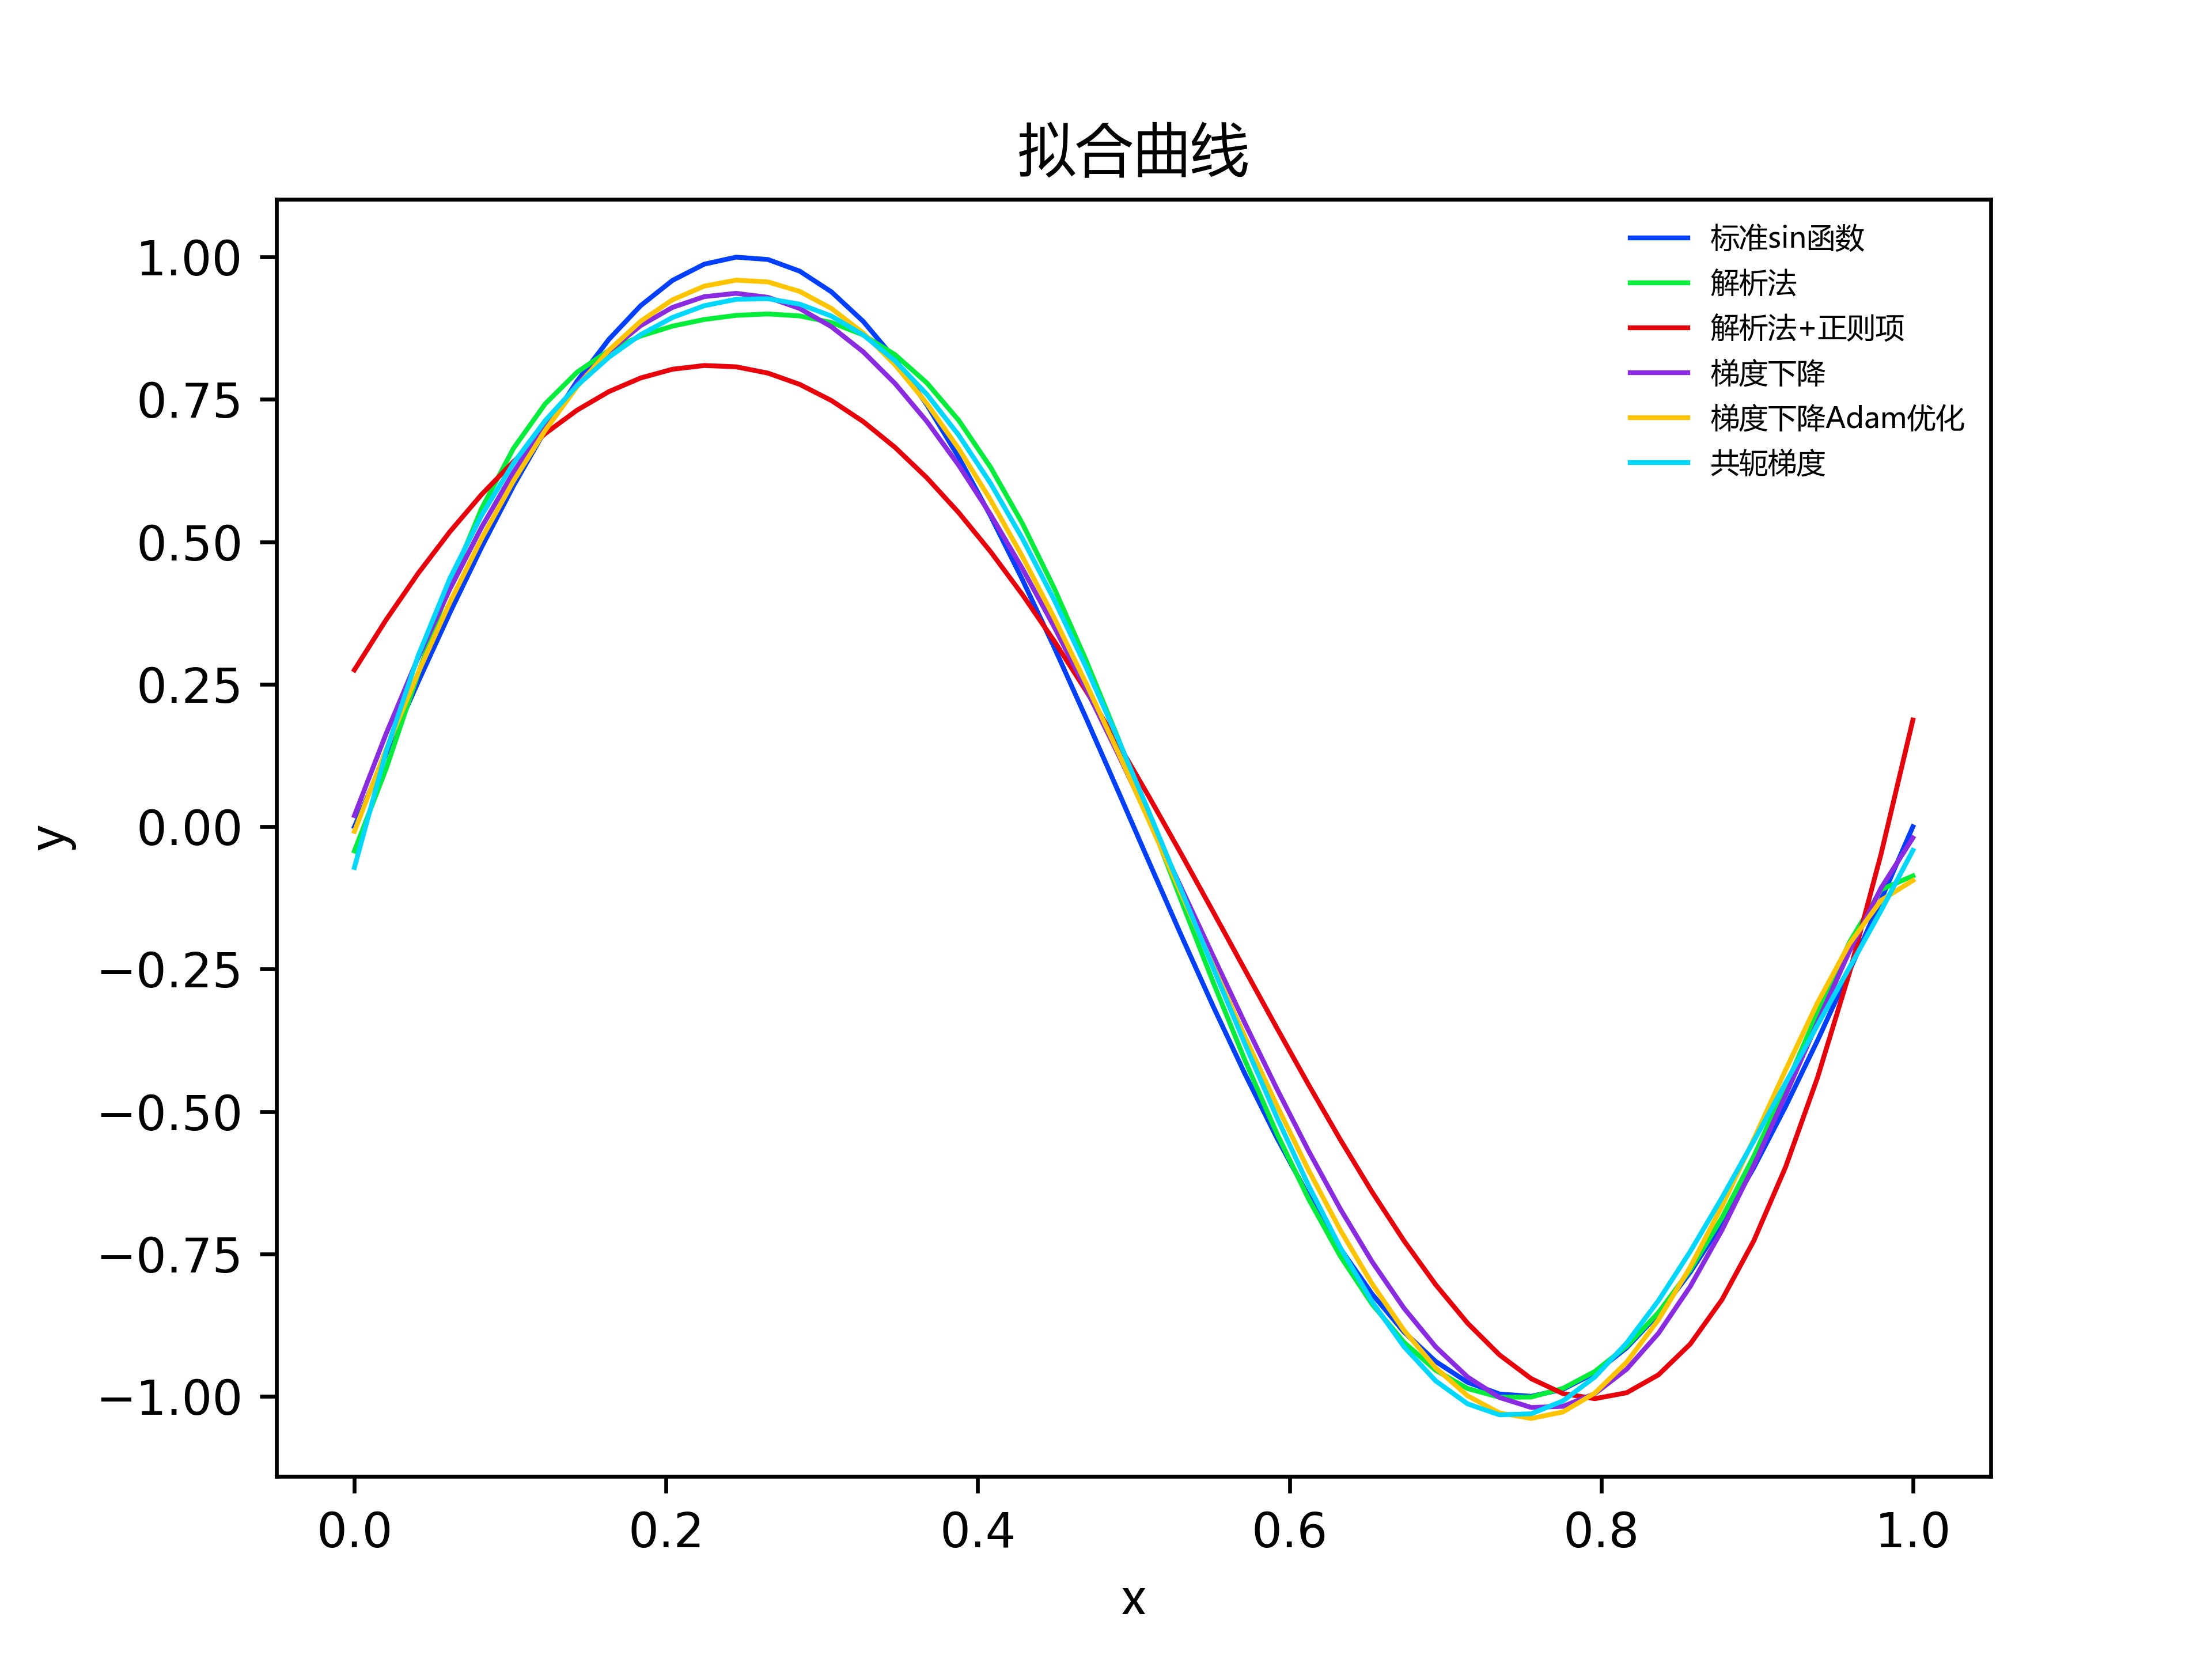
\includegraphics[width=0.3\textwidth]{n50o9}
}
\caption{n=50 不同阶拟合曲线}
\end{figure}

实验数据继续增加,此时可以发现带正则项的方法与其他方法拟合效果的差距已经在一个较小的范围内,而正则项系数并未变化,符合课堂上提到的正则项仅作为先验出现,会随着实验数据量逐渐增加而减小,从公式中也可以看出正则项对损失函数影响不会随数据集的增大而增大,反而相对减小。

\newpage
当数据集大小为100时,取多项式阶数为2,3,5,7,8,9。其拟合曲线及拟合优度如下。
\linespread{1.2}
\begin{table}[H]  
  \centering  
  \begin{threeparttable}  
  \caption{n=100 不同阶拟合优度}  
  \label{tab:performance_comparison} 
  \begin{tabular}{m{0.1\textwidth}<{\centering} m{0.15\textwidth}<{\centering} m{0.15\textwidth}<{\centering} m{0.15\textwidth}<{\centering} m{0.15\textwidth}<{\centering} m{0.15\textwidth}<{\centering}}  
    \toprule[1.5pt]  
    \multirow{2}{*}{阶数}&\multicolumn{2}{c}{解析法}&\multicolumn{2}{c}{梯度下降} &\multirow{2}{*}{共轭梯度}\cr  
    \cmidrule(lr){2-3} \cmidrule(lr){4-5}  
    &不含正则项&含正则项&未优化&优化后\cr  
    \midrule  
2&0.6382&0.6380&0.6379&0.6382&0.6382\cr
3&0.1014&0.2499&0.1012&0.1014&0.1014\cr
5&0.0461&0.1793&0.1233&0.0819&0.0461\cr
7&0.0210&0.1755&0.0777&0.0290&0.0178\cr
8&0.0470&0.1639&0.0784&0.0469&0.0448\cr
9&0.0284&0.1206&0.0494&0.0370&0.0255\cr
    \bottomrule  
    \end{tabular}  
    \end{threeparttable}  
\end{table}

\begin{figure}[H]
\centering
\subfigure[2阶]{
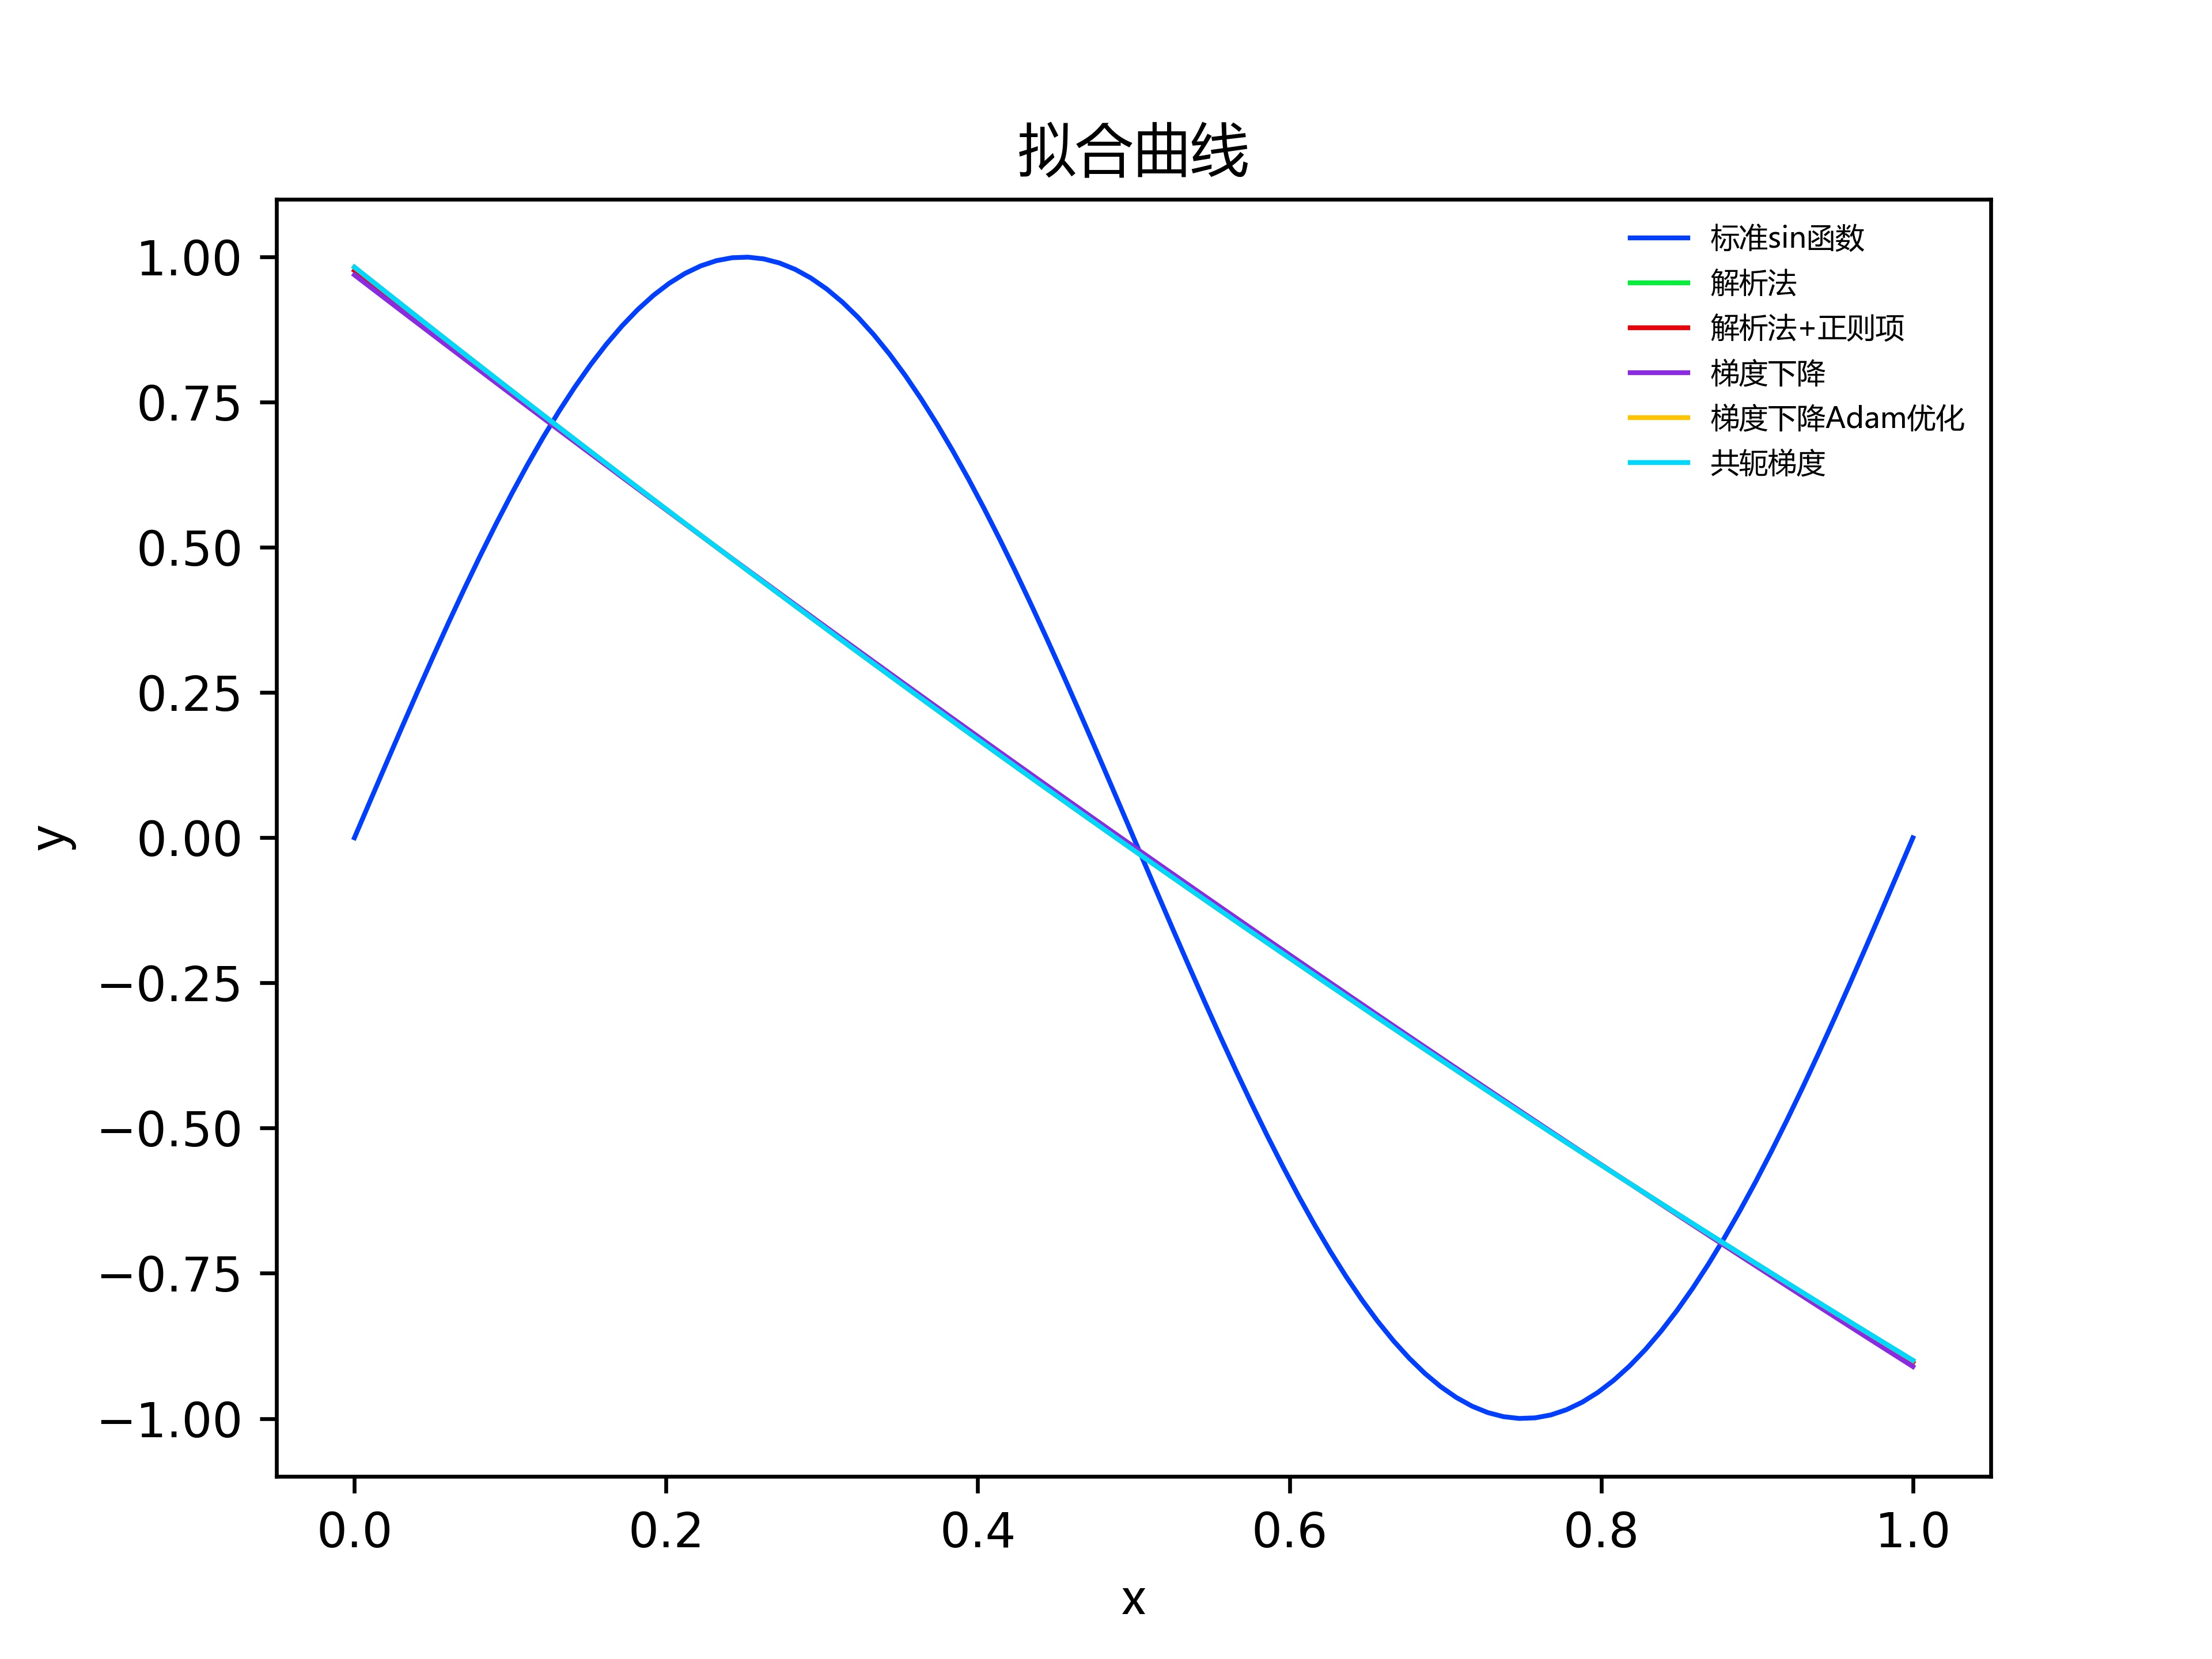
\includegraphics[width=0.3\textwidth]{n100o2}
}
\subfigure[3阶]{
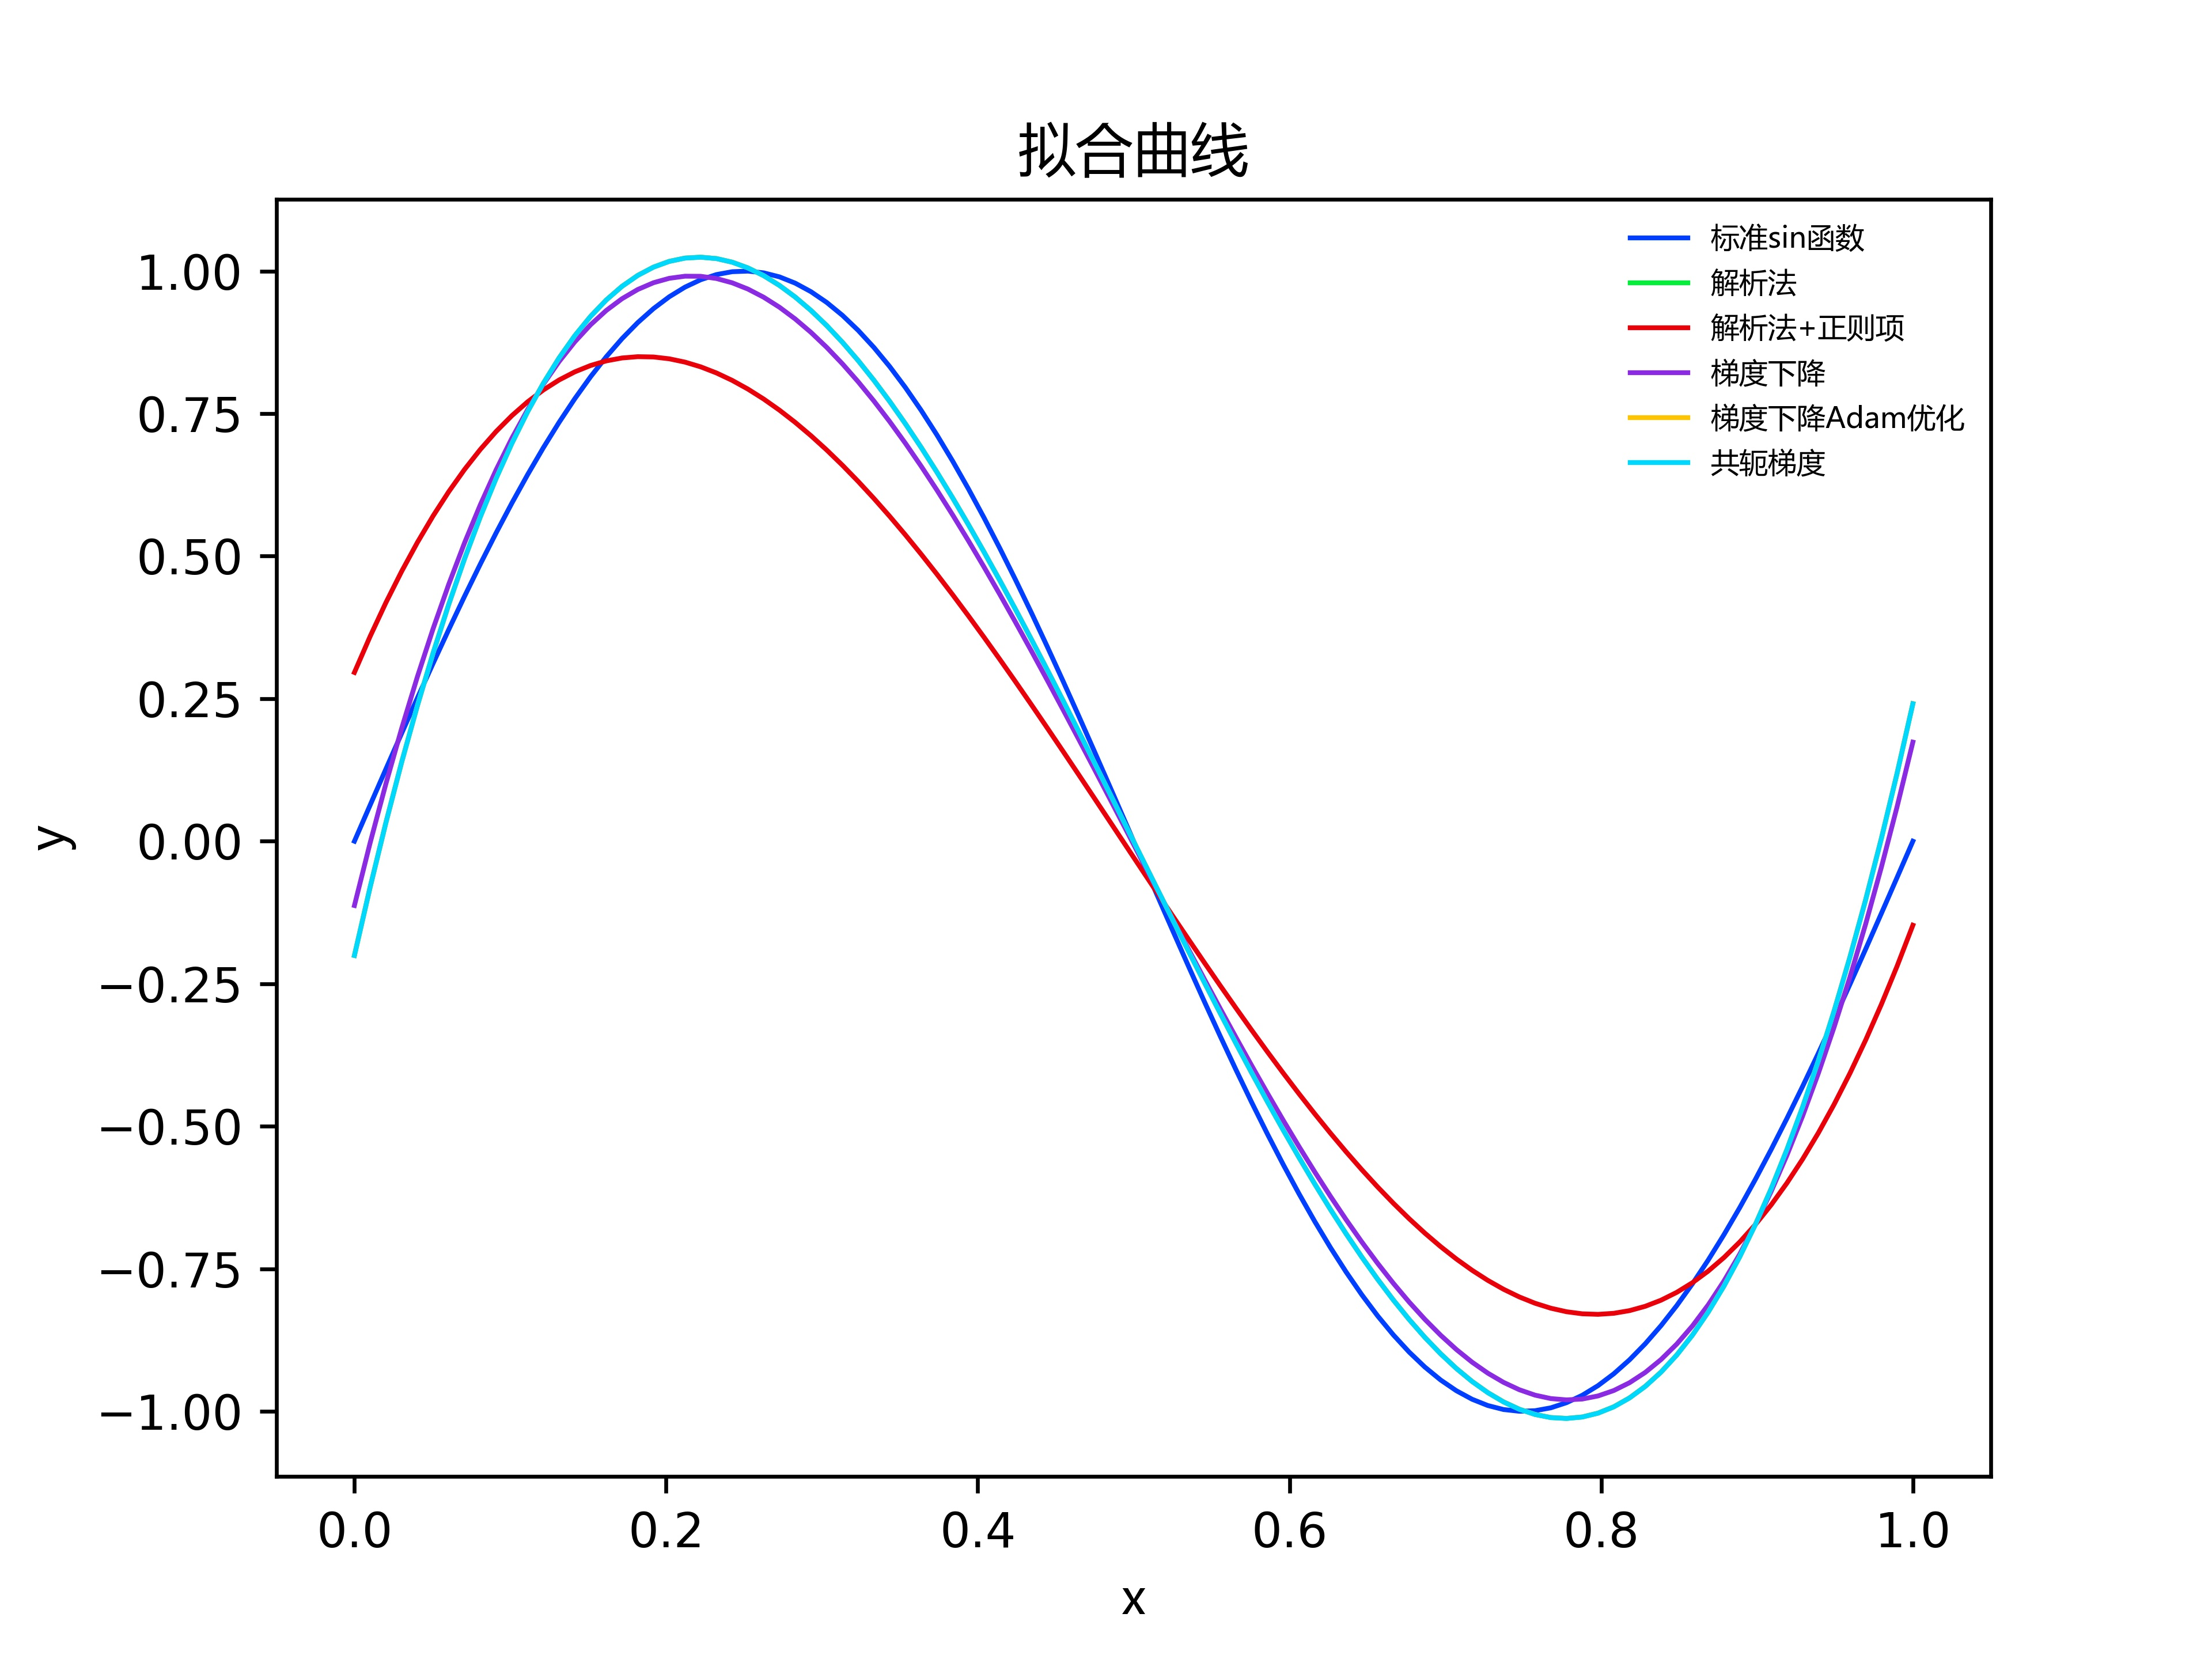
\includegraphics[width=0.3\textwidth]{n100o3}
}
\subfigure[5阶]{
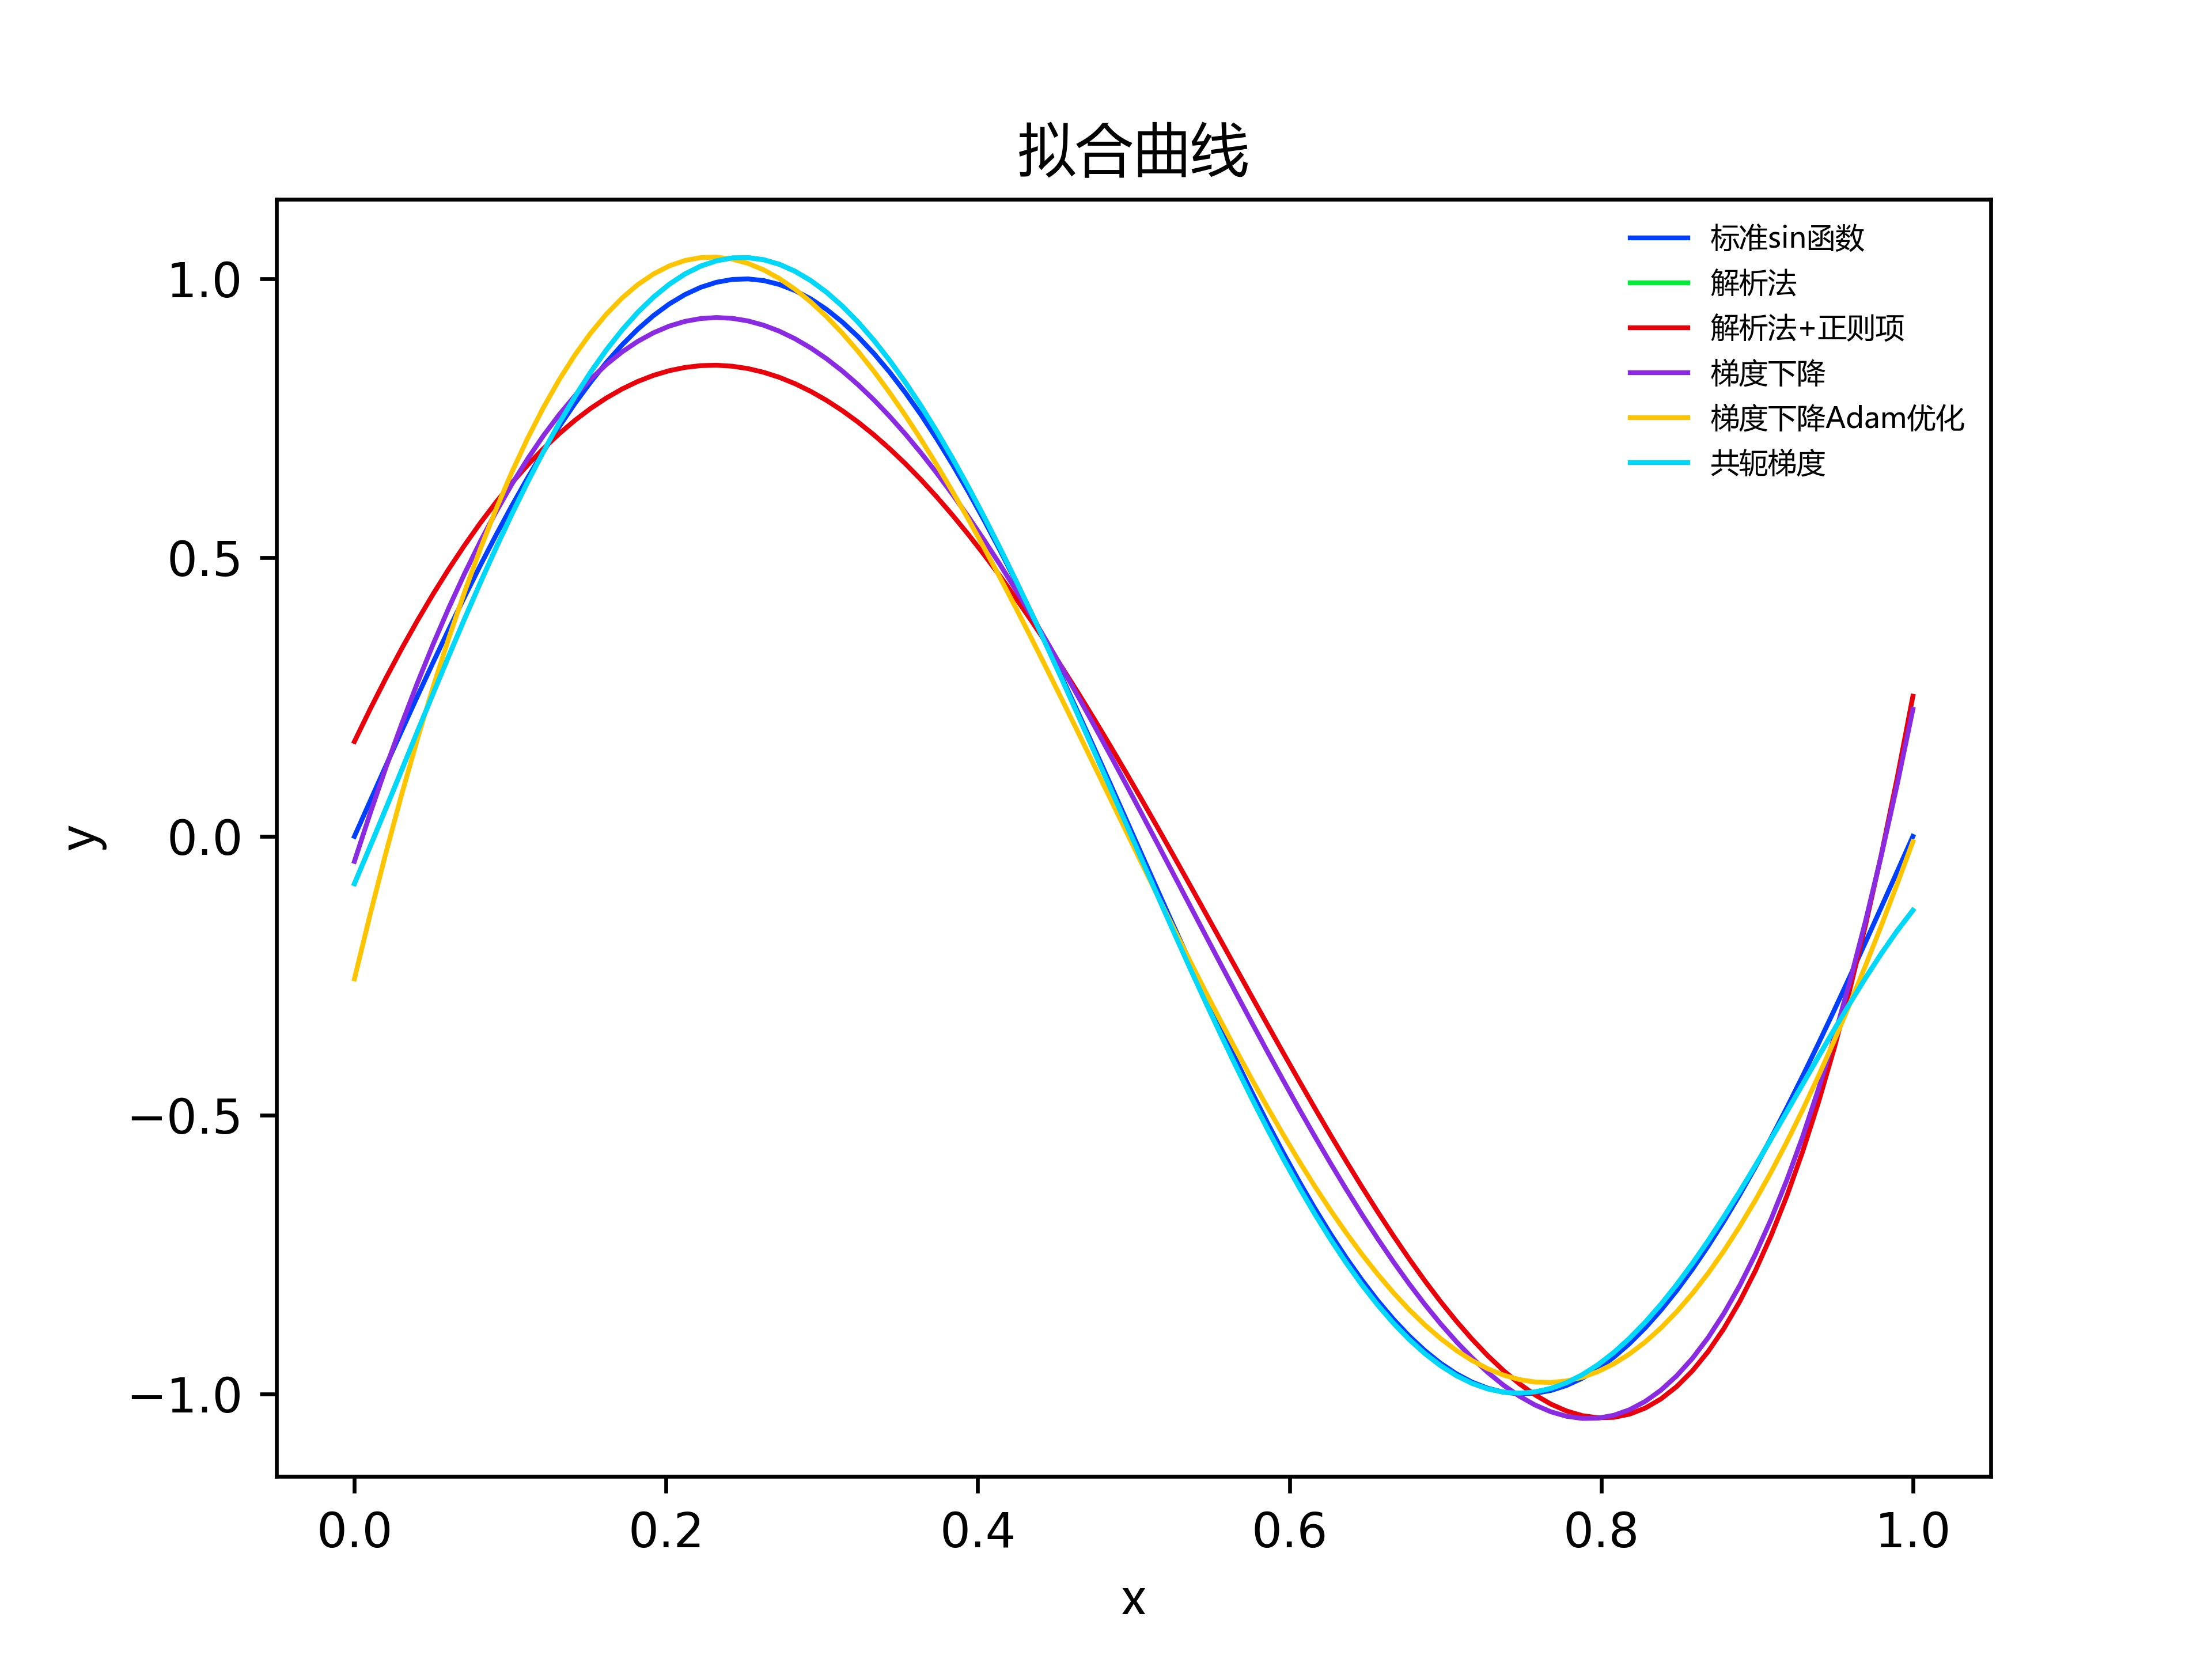
\includegraphics[width=0.3\textwidth]{n100o5}
}
\quad
\subfigure[7阶]{
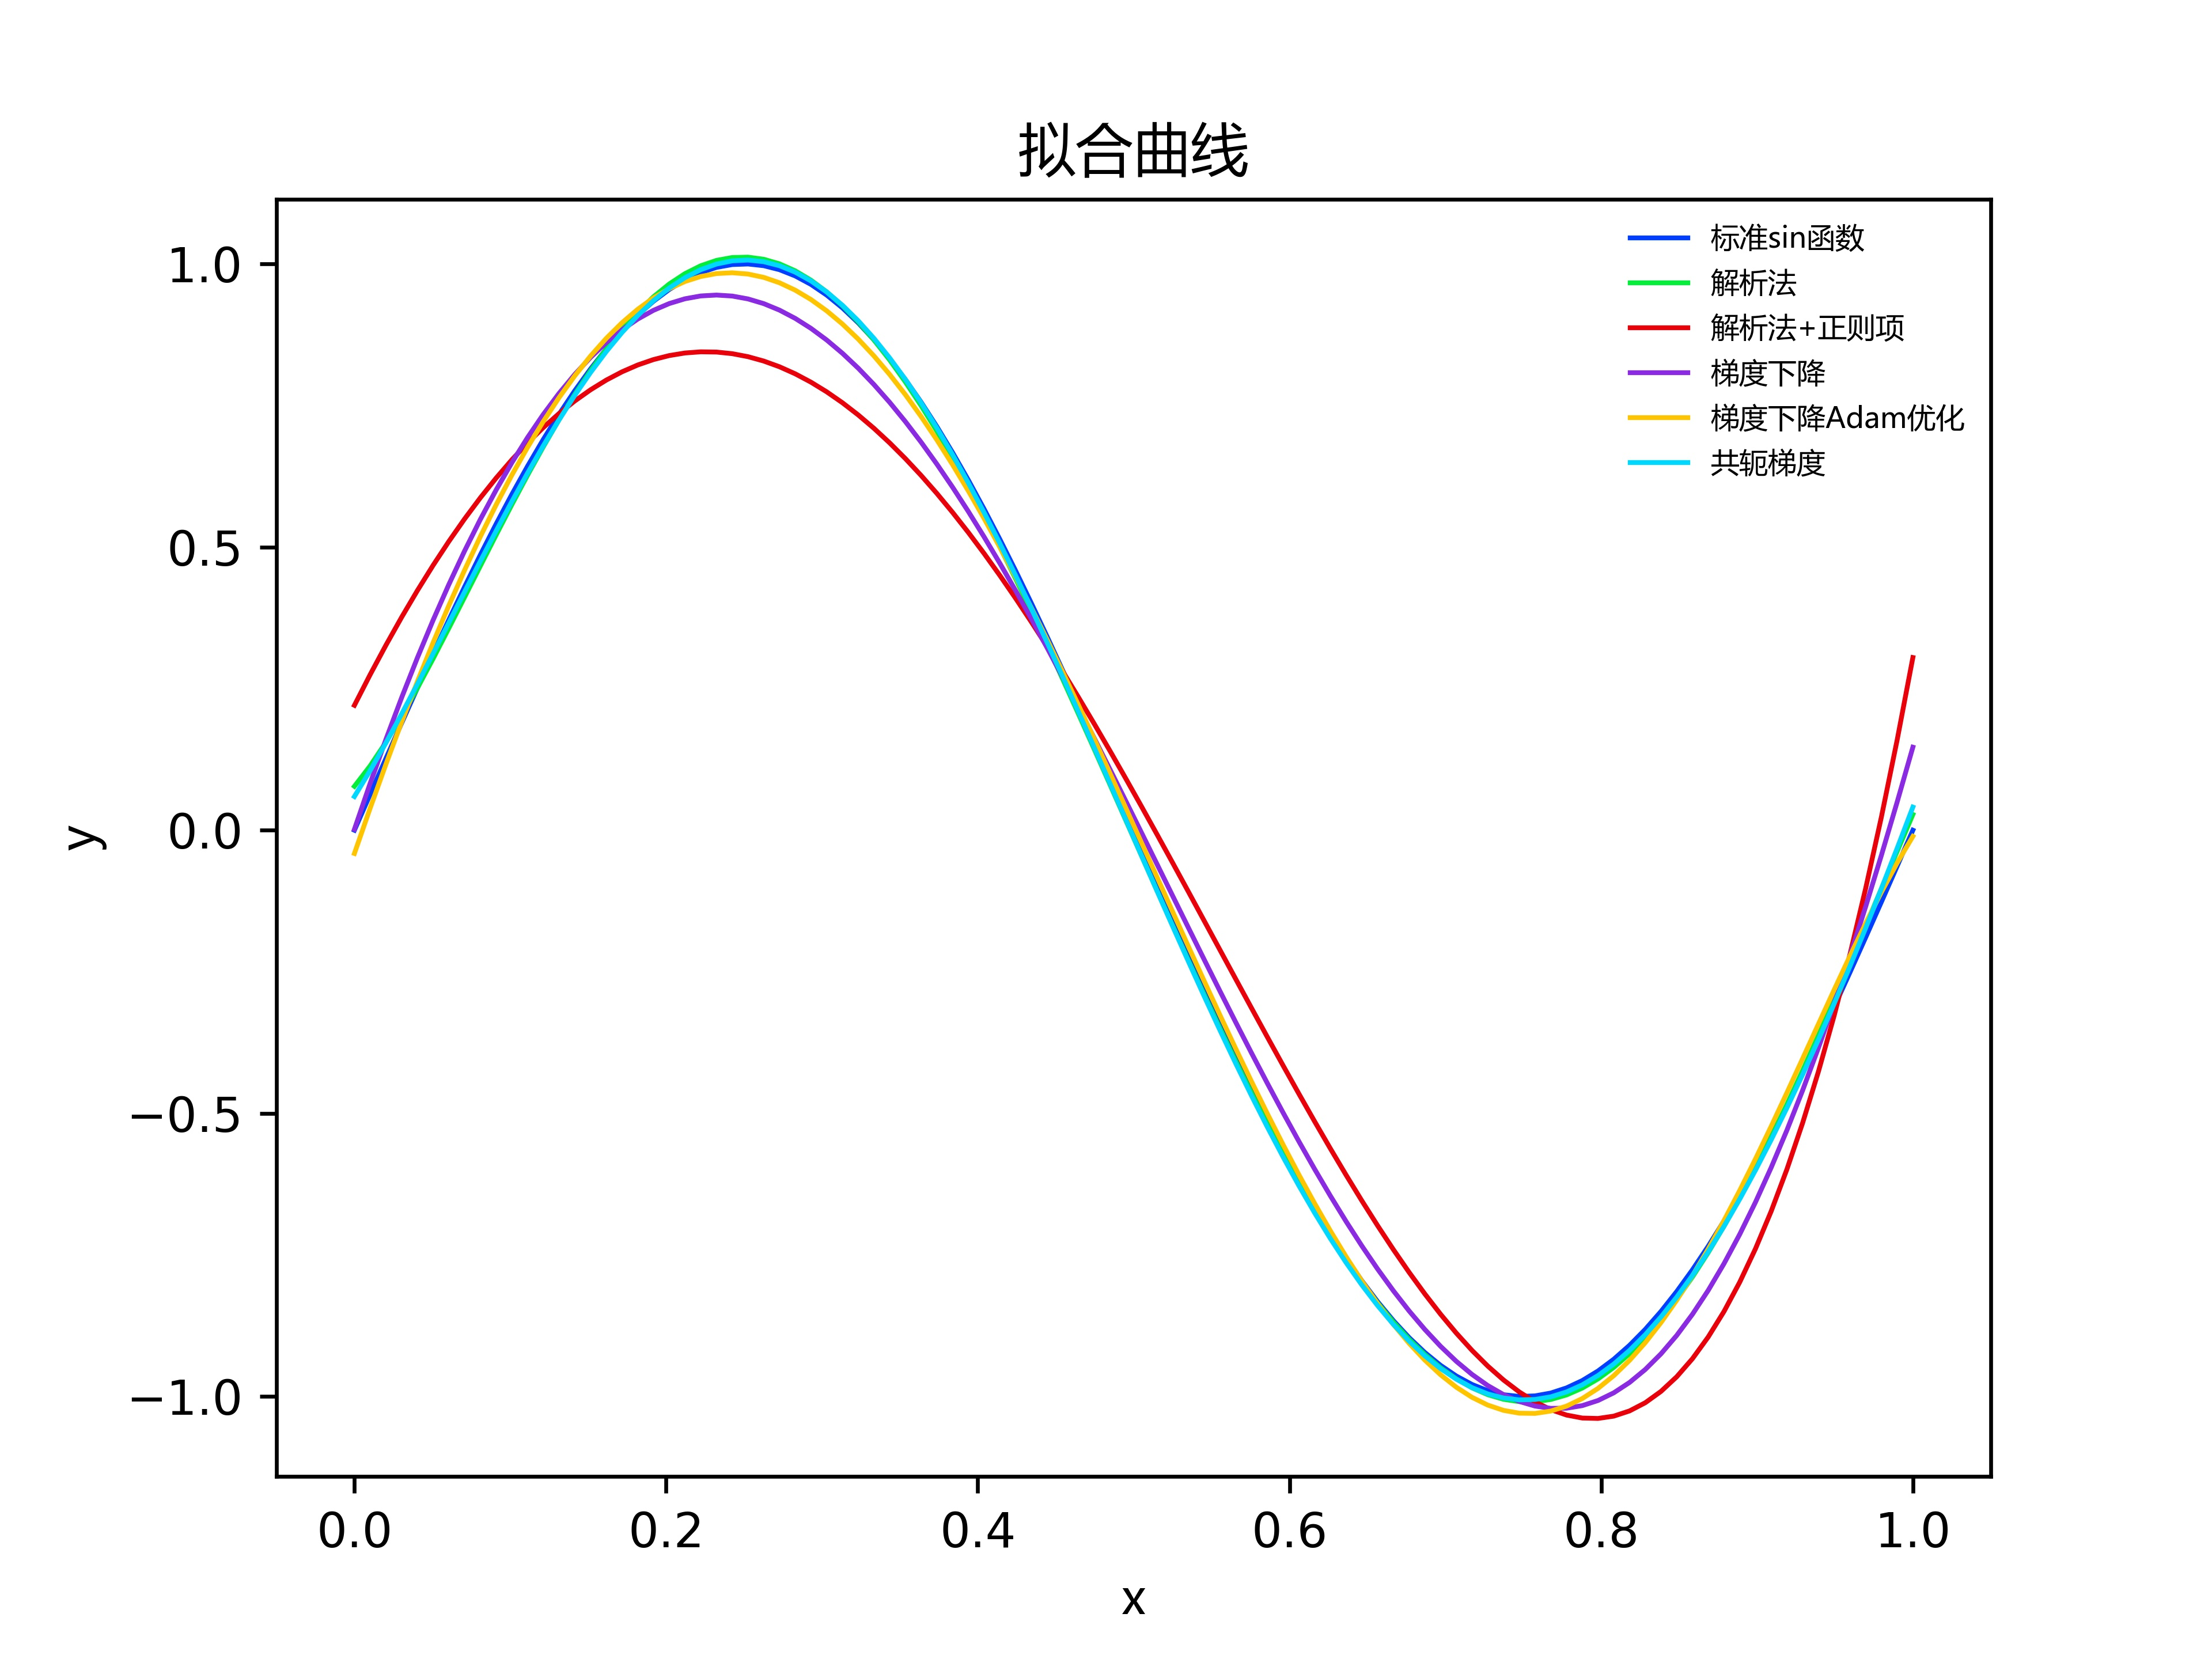
\includegraphics[width=0.3\textwidth]{n100o7}
}
\subfigure[8阶]{
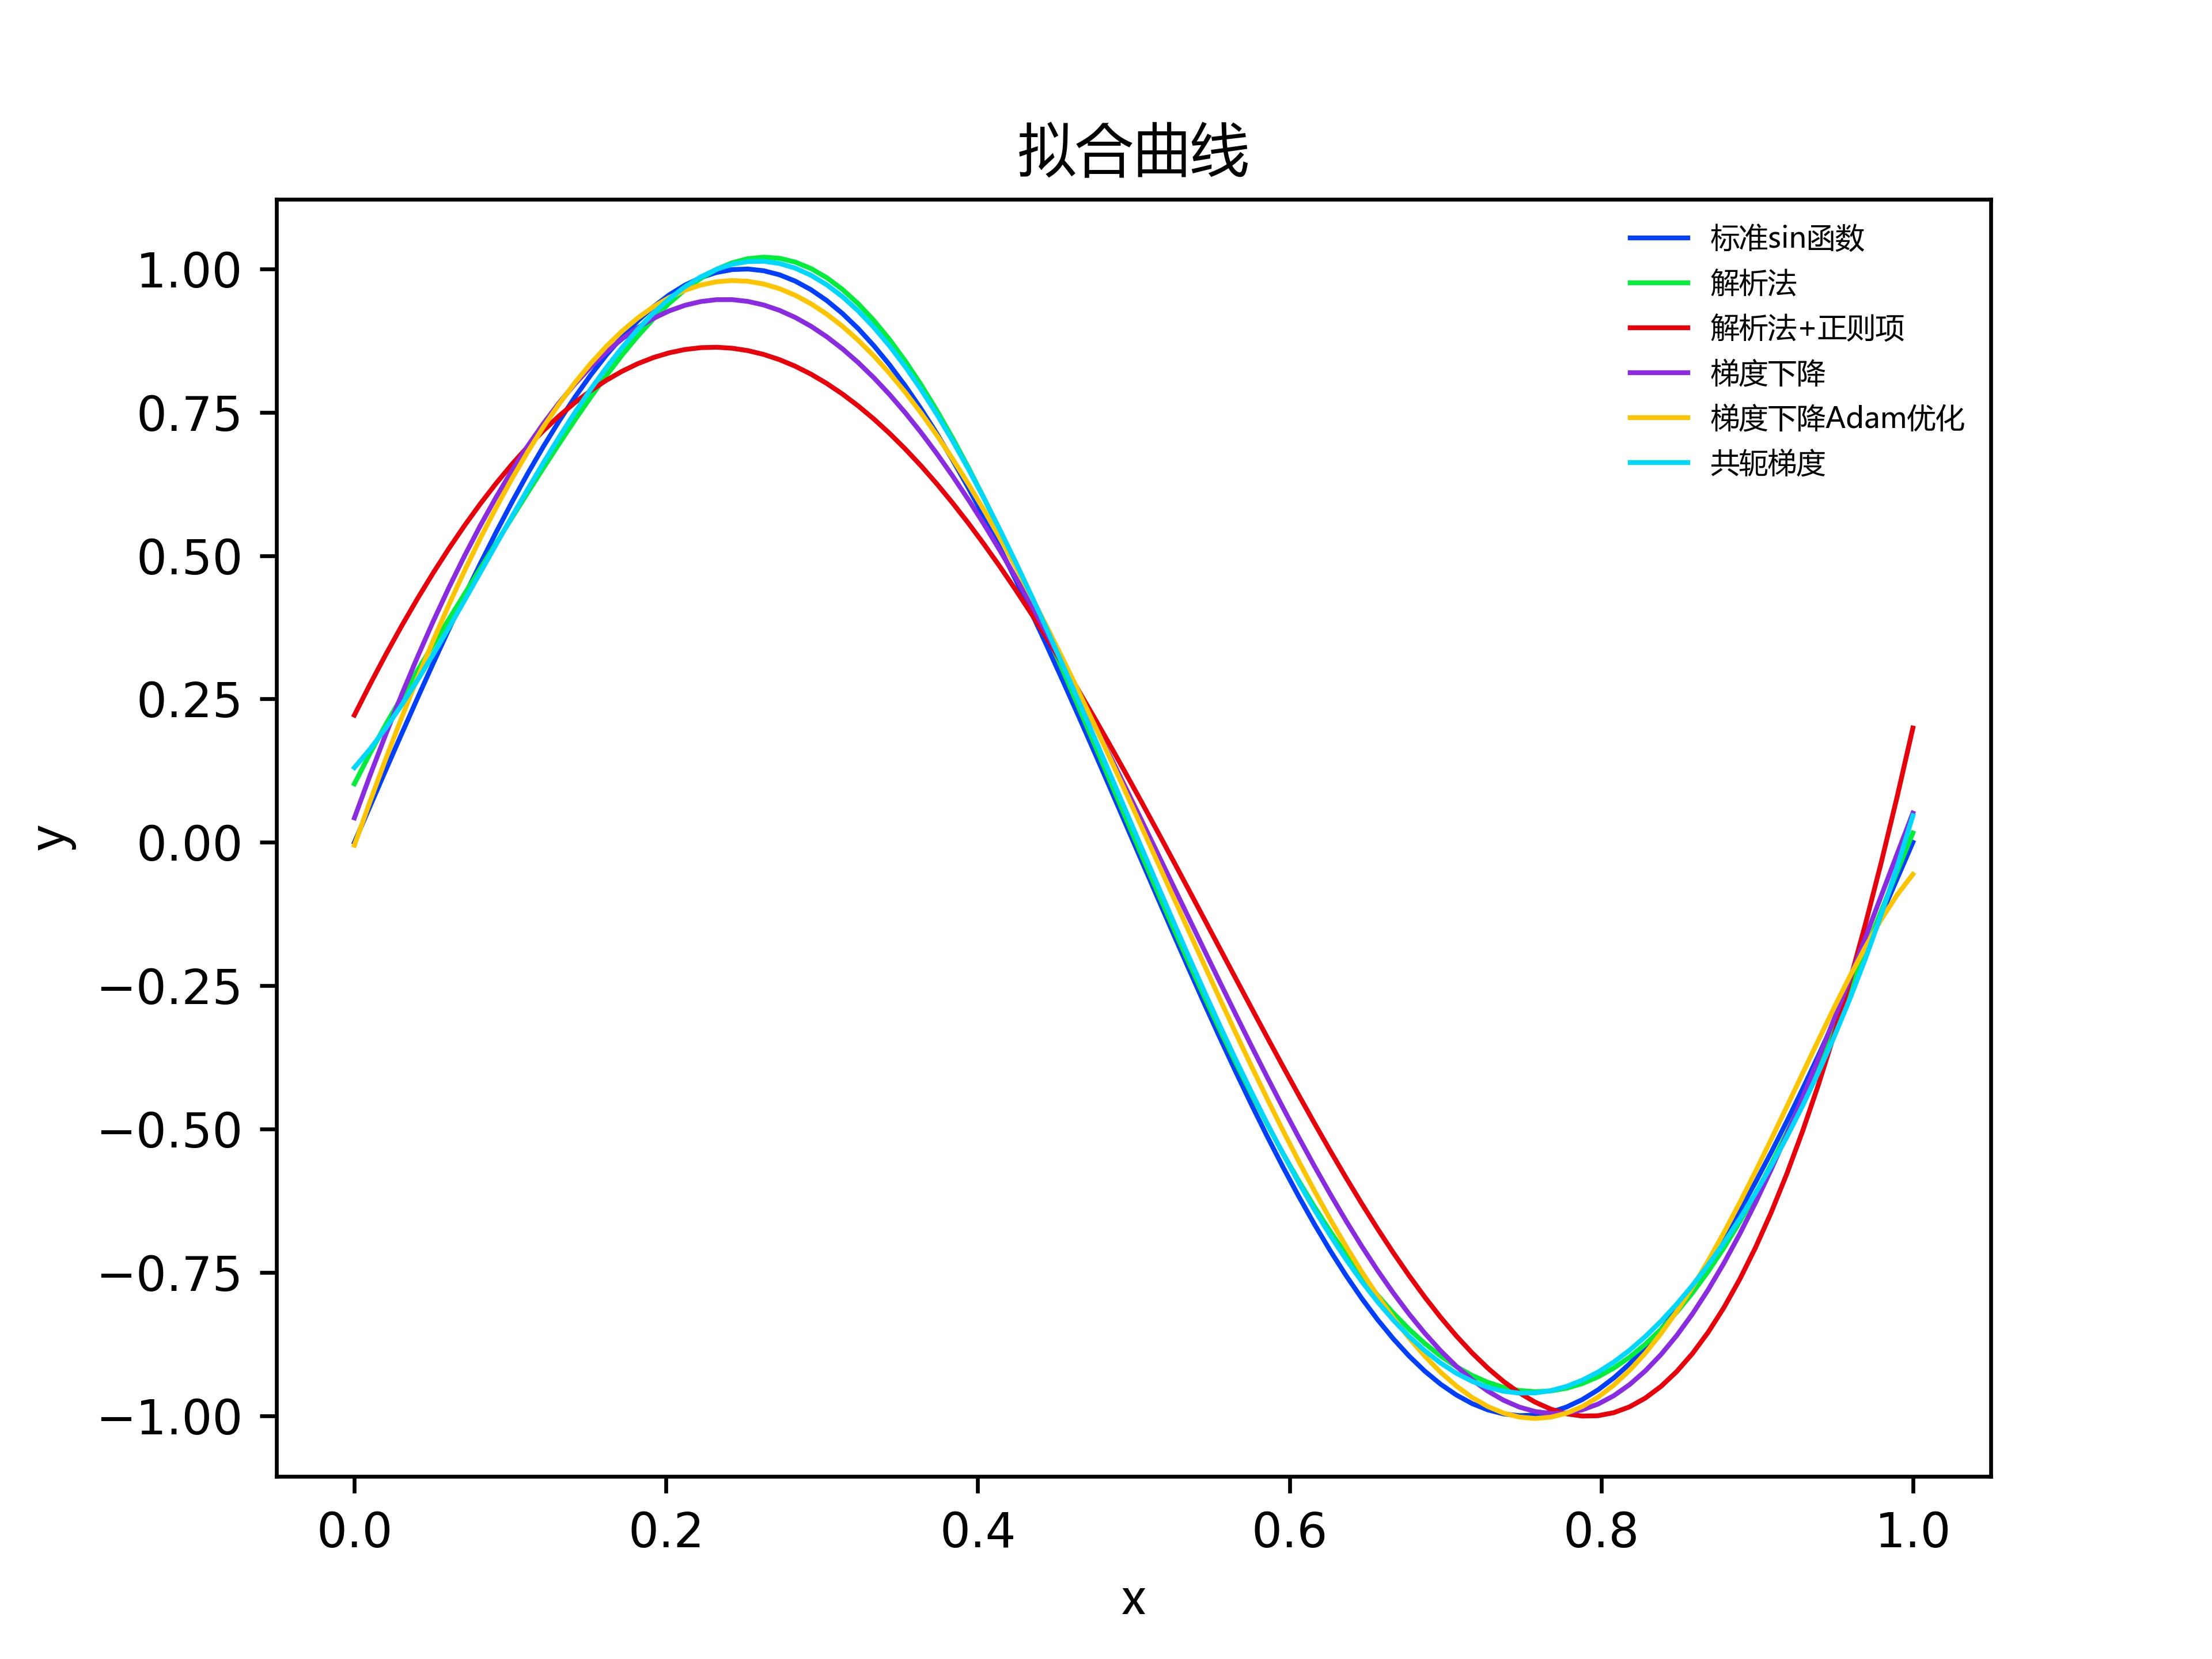
\includegraphics[width=0.3\textwidth]{n100o8}
}
\subfigure[9阶]{
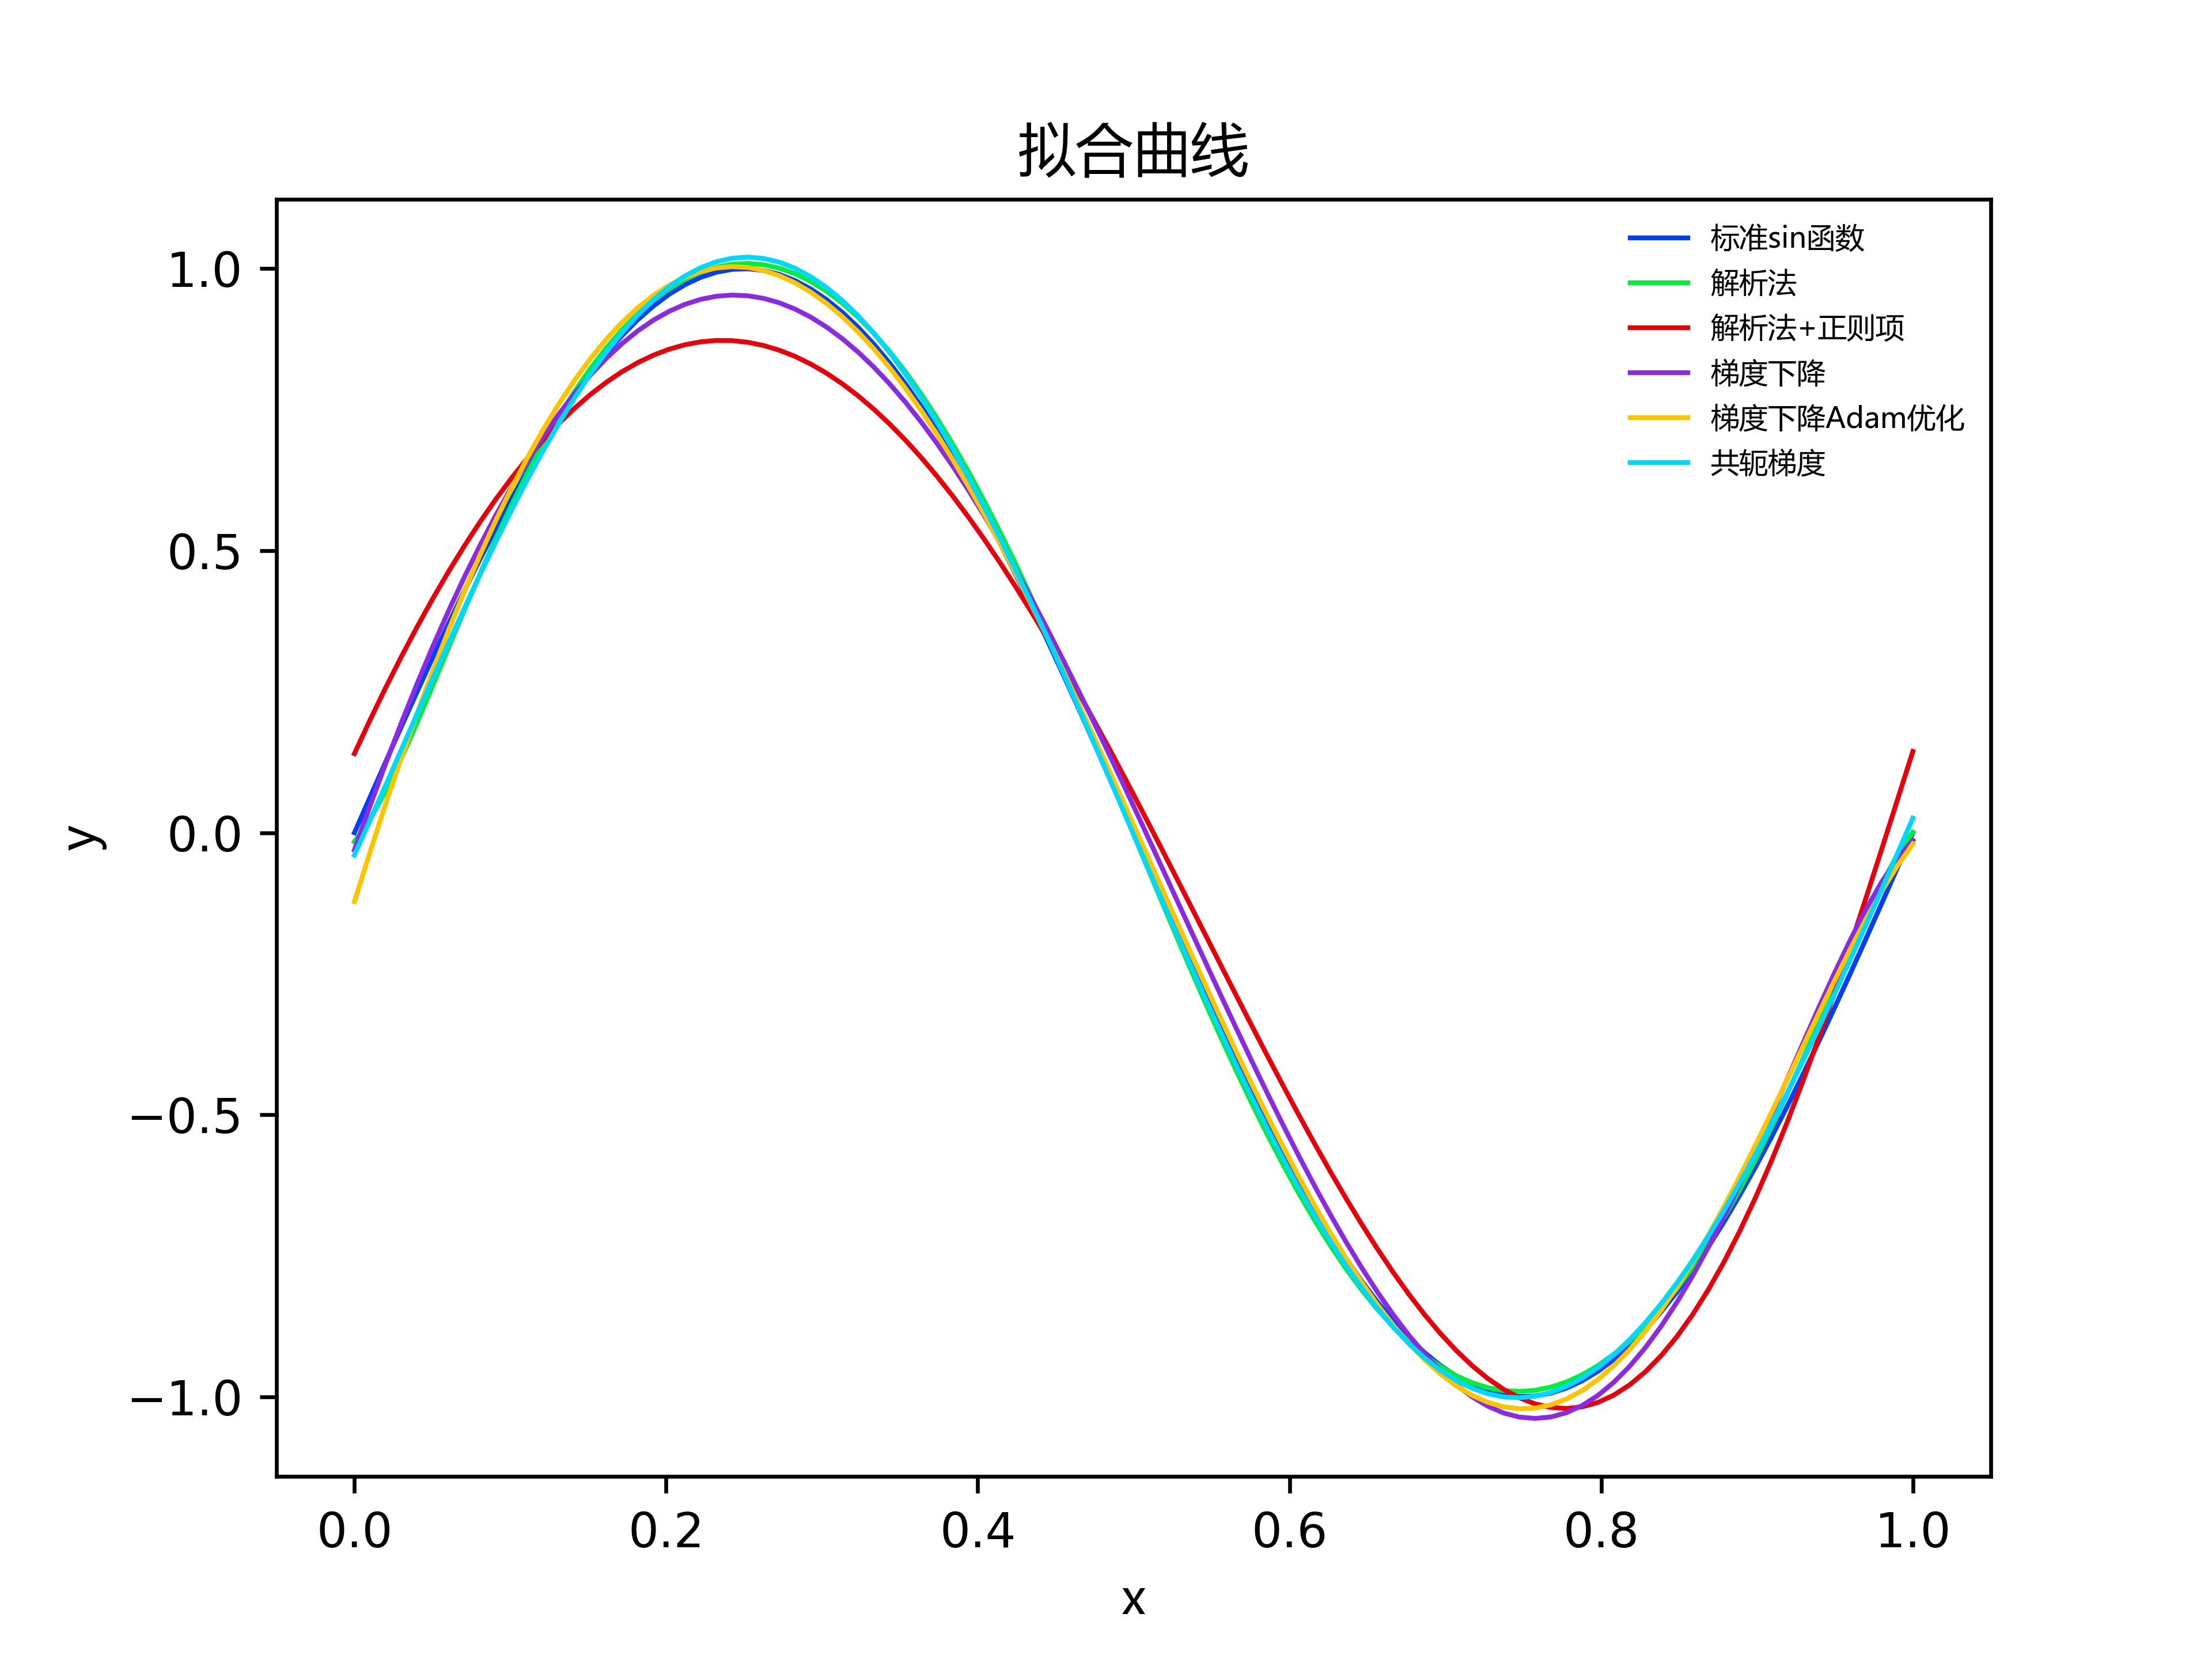
\includegraphics[width=0.3\textwidth]{n100o9}
}
\caption{n=100 不同阶拟合曲线}
\end{figure}
此时正则项的影响继续减少,但仍差于其他方法,因此此时设置的正则项系数是过大的。同时实验中观察了不同数据集,不同阶数下的用时,发现运行时间受数据集大小影响较大,受阶数影响较小。而用时较多主要是梯度下降方法,其采用批量梯度下降的方法对内存要求较高,迭代一次所用时间会随着数据集大小增大而增大,与实验结果吻合。

\subsection{不同超参数效果}
\subsubsection{梯度下降中学习率对拟合效果的影响}
为了凸显梯度下降中学习率对拟合效果的影响,取数据集大小为20,阶数为5,迭代次数为40000,无正则项,无优化。学习率取值分别为$\eta=0.01,0,05,0.1,0.5,0.9$,实验得到不同学习率下的拟合优度大小和拟合情况。

\linespread{1.2}
\begin{table}[H]
\centering
\caption{学习率对拟合优度的影响}
\label{tab:performance_comparison}
\begin{tabular}{cccccc}
\toprule[1.5pt]
\makebox[0.15\textwidth][c]{学习率}&\makebox[0.15\textwidth][c]{0.01} &\makebox[0.15\textwidth][c]{0.05}&\makebox[0.15\textwidth][c]{0.1}&\makebox[0.15\textwidth][c]{0.5}&\makebox[0.15\textwidth][c]{0.9}\\ \hline
拟合优度&0.4642&0.2444&0.2118&0.1635&0.1316 \\
\bottomrule[1.5pt]
\end{tabular}
\end{table}

\begin{figure}[H]
    \centering
    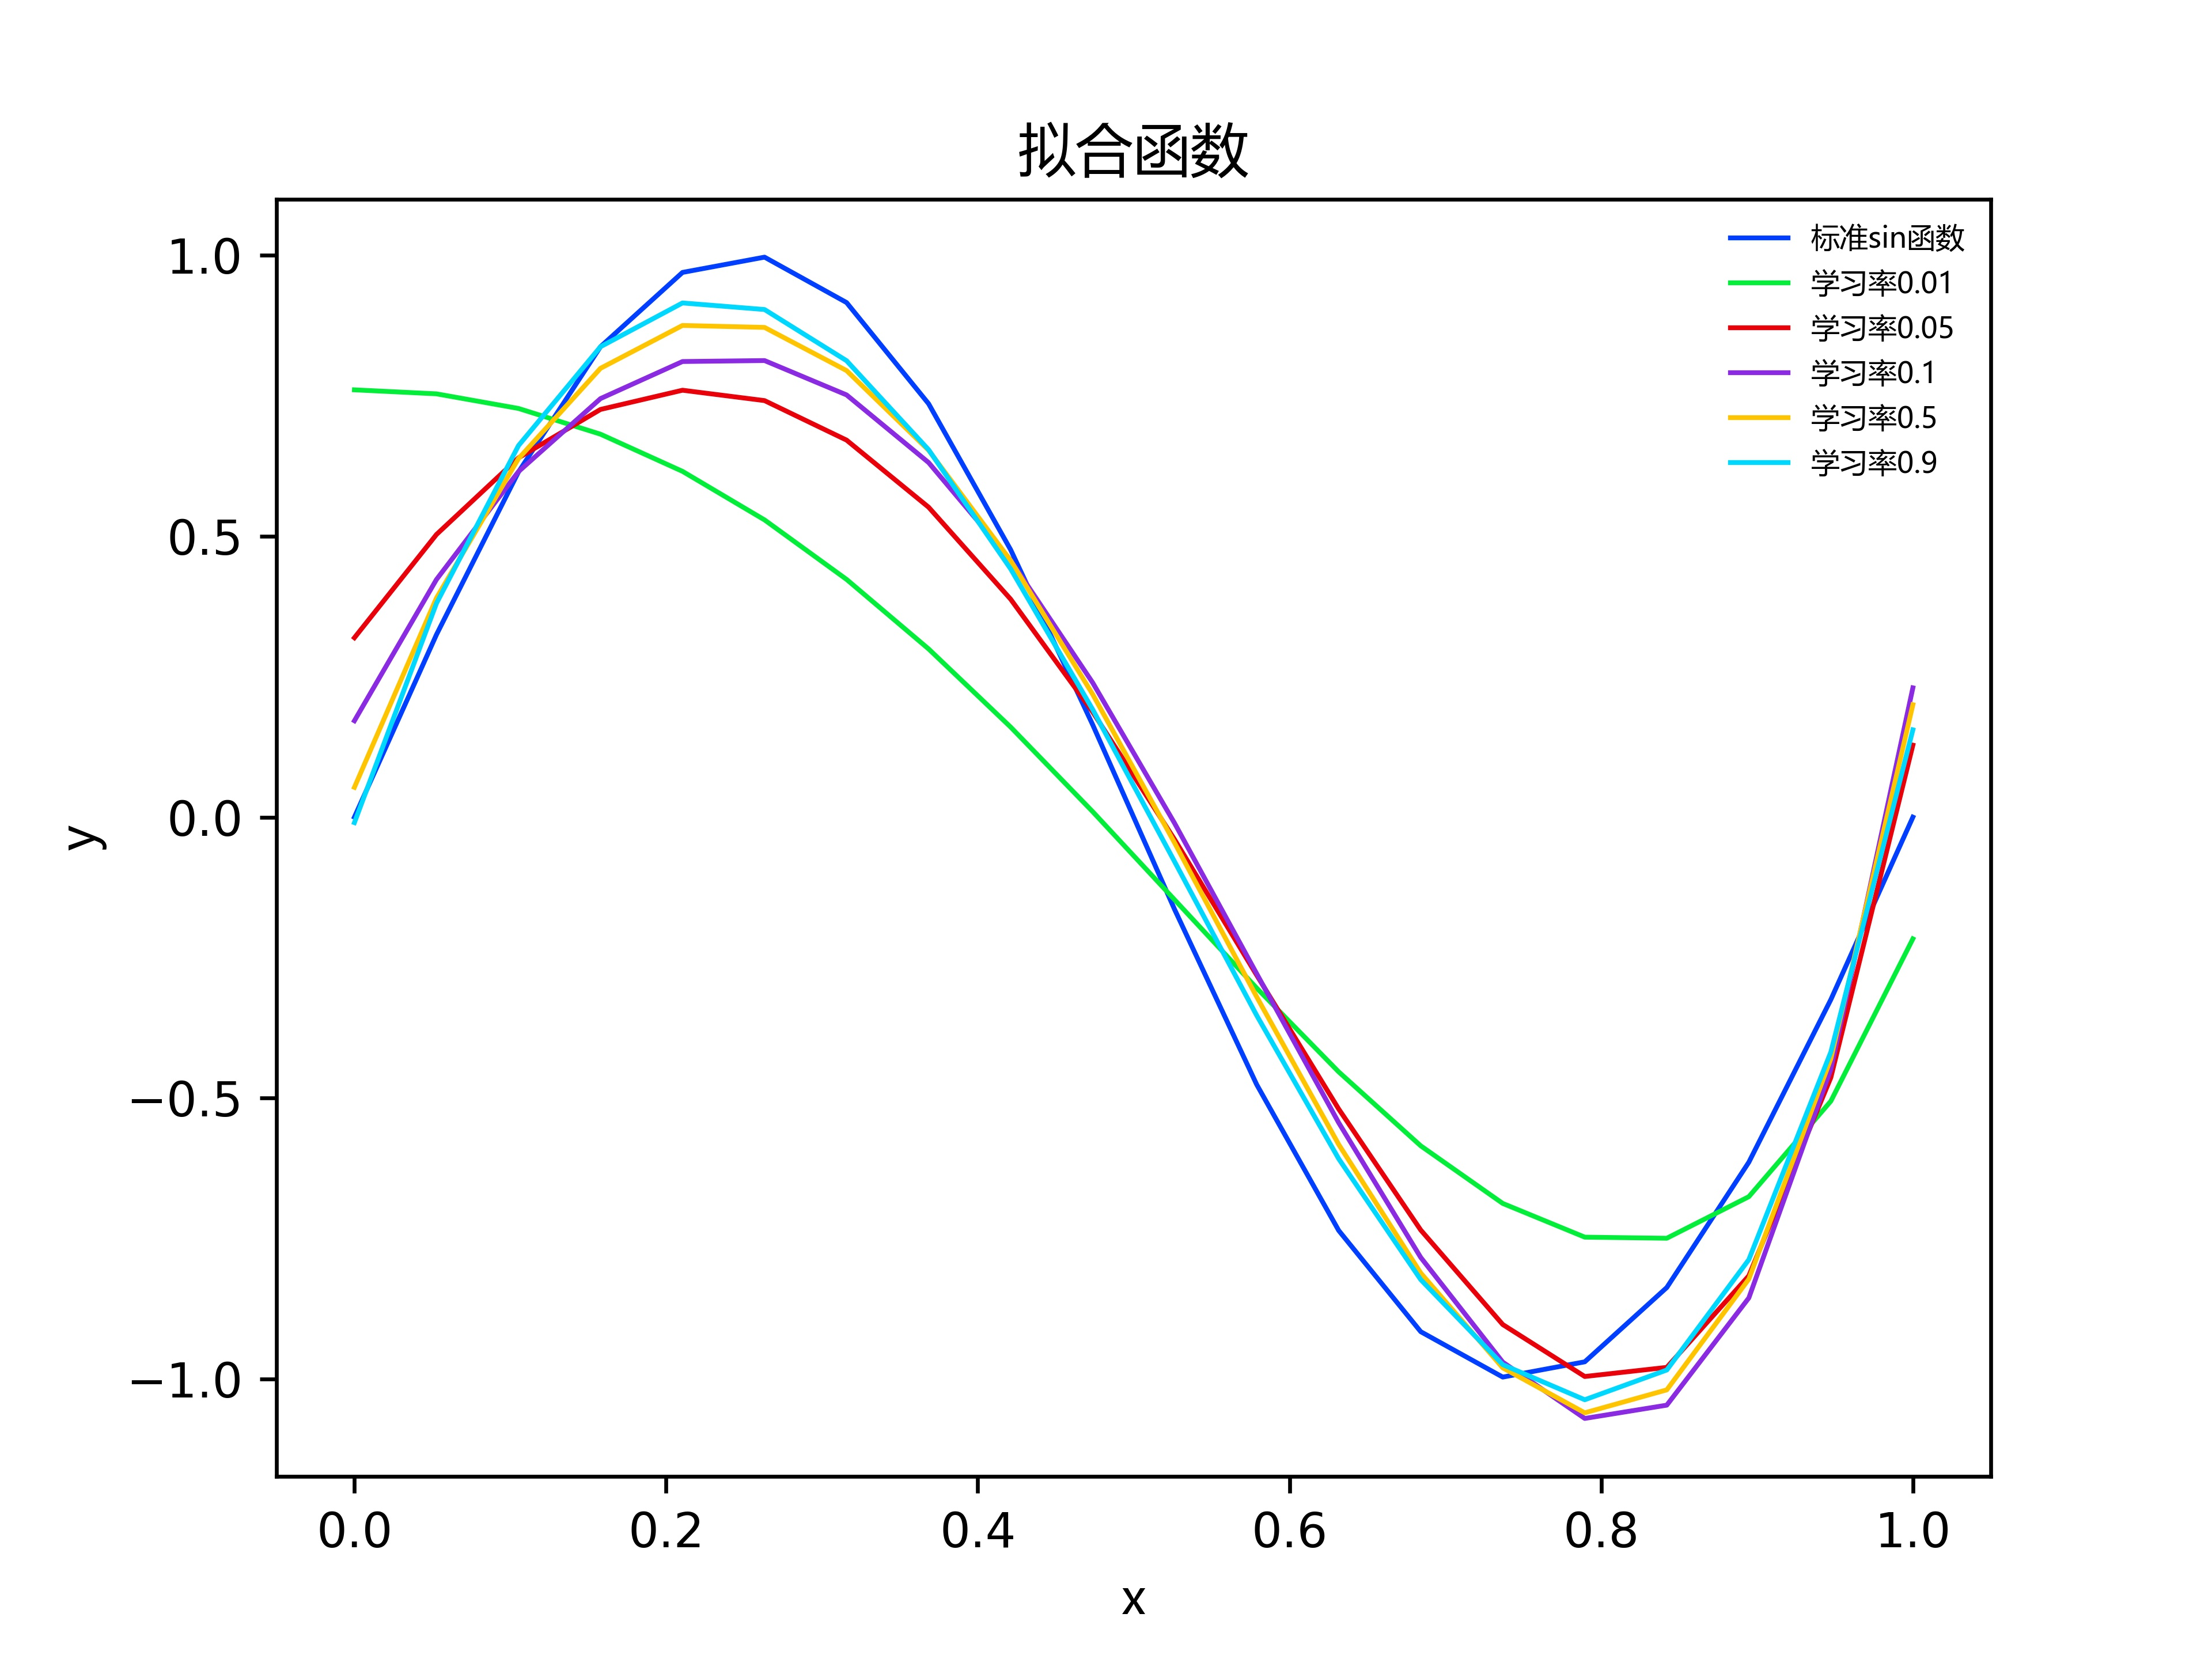
\includegraphics[width=0.88\textwidth]{n20o5学习率}
    \caption{不同学习率下拟合曲线}
    \label{图4}
\end{figure}

依据拟合优度,结合之前实验数据,可以出此时并未达到收敛。随着学习率的增加,曲线拟合的效果越来越好好,拟合优度也越小。

\subsubsection{解析法中正则项比率对过拟合效果的影响}
在上述实验中已经发现不带正则项的解析法效果普遍较好,带正则项的情况下由于正则项过大导致拟合效果欠佳。为凸显正则项的效果,可以将数据集大小限制在较小范围内。故此次取数据集大小为10,阶数为12,上述实验中已经可以看出解析法的拟合效果是最好的,而且在阶数为9的情况下明显出现了过拟合的情况,可以认为此时同样出现了过拟合的情况。此时正则项系数取值分别为$\lambda=0,e^{-10},e^{-5},e^{-1}$。拟合情况如下所示。

\linespread{1.2}
\begin{table}[H]
\centering
\caption{正则项系数对拟合优度的影响}
\label{tab:performance_comparison}  %可能是自动编号
\begin{tabular}{ccccc} %cc表示有两行,中见加|,则表格中就会多一条竖线
\toprule[1.5pt] %加粗
 \makebox[0.17\textwidth][c]{正则项系数}	&  \makebox[0.17\textwidth][c]{0} &  \makebox[0.17\textwidth][c]{$e^{-10}$} &  \makebox[0.17\textwidth][c]{$e^{-5}$}
&  \makebox[0.17\textwidth][c]{$e^{-1}$}\\ \hline
拟合优度&0.6117&0.068433&0.3304&0.5815  \\
\bottomrule[1.5pt] %加粗
\end{tabular}
\end{table}

\begin{figure}[H]
    \centering
    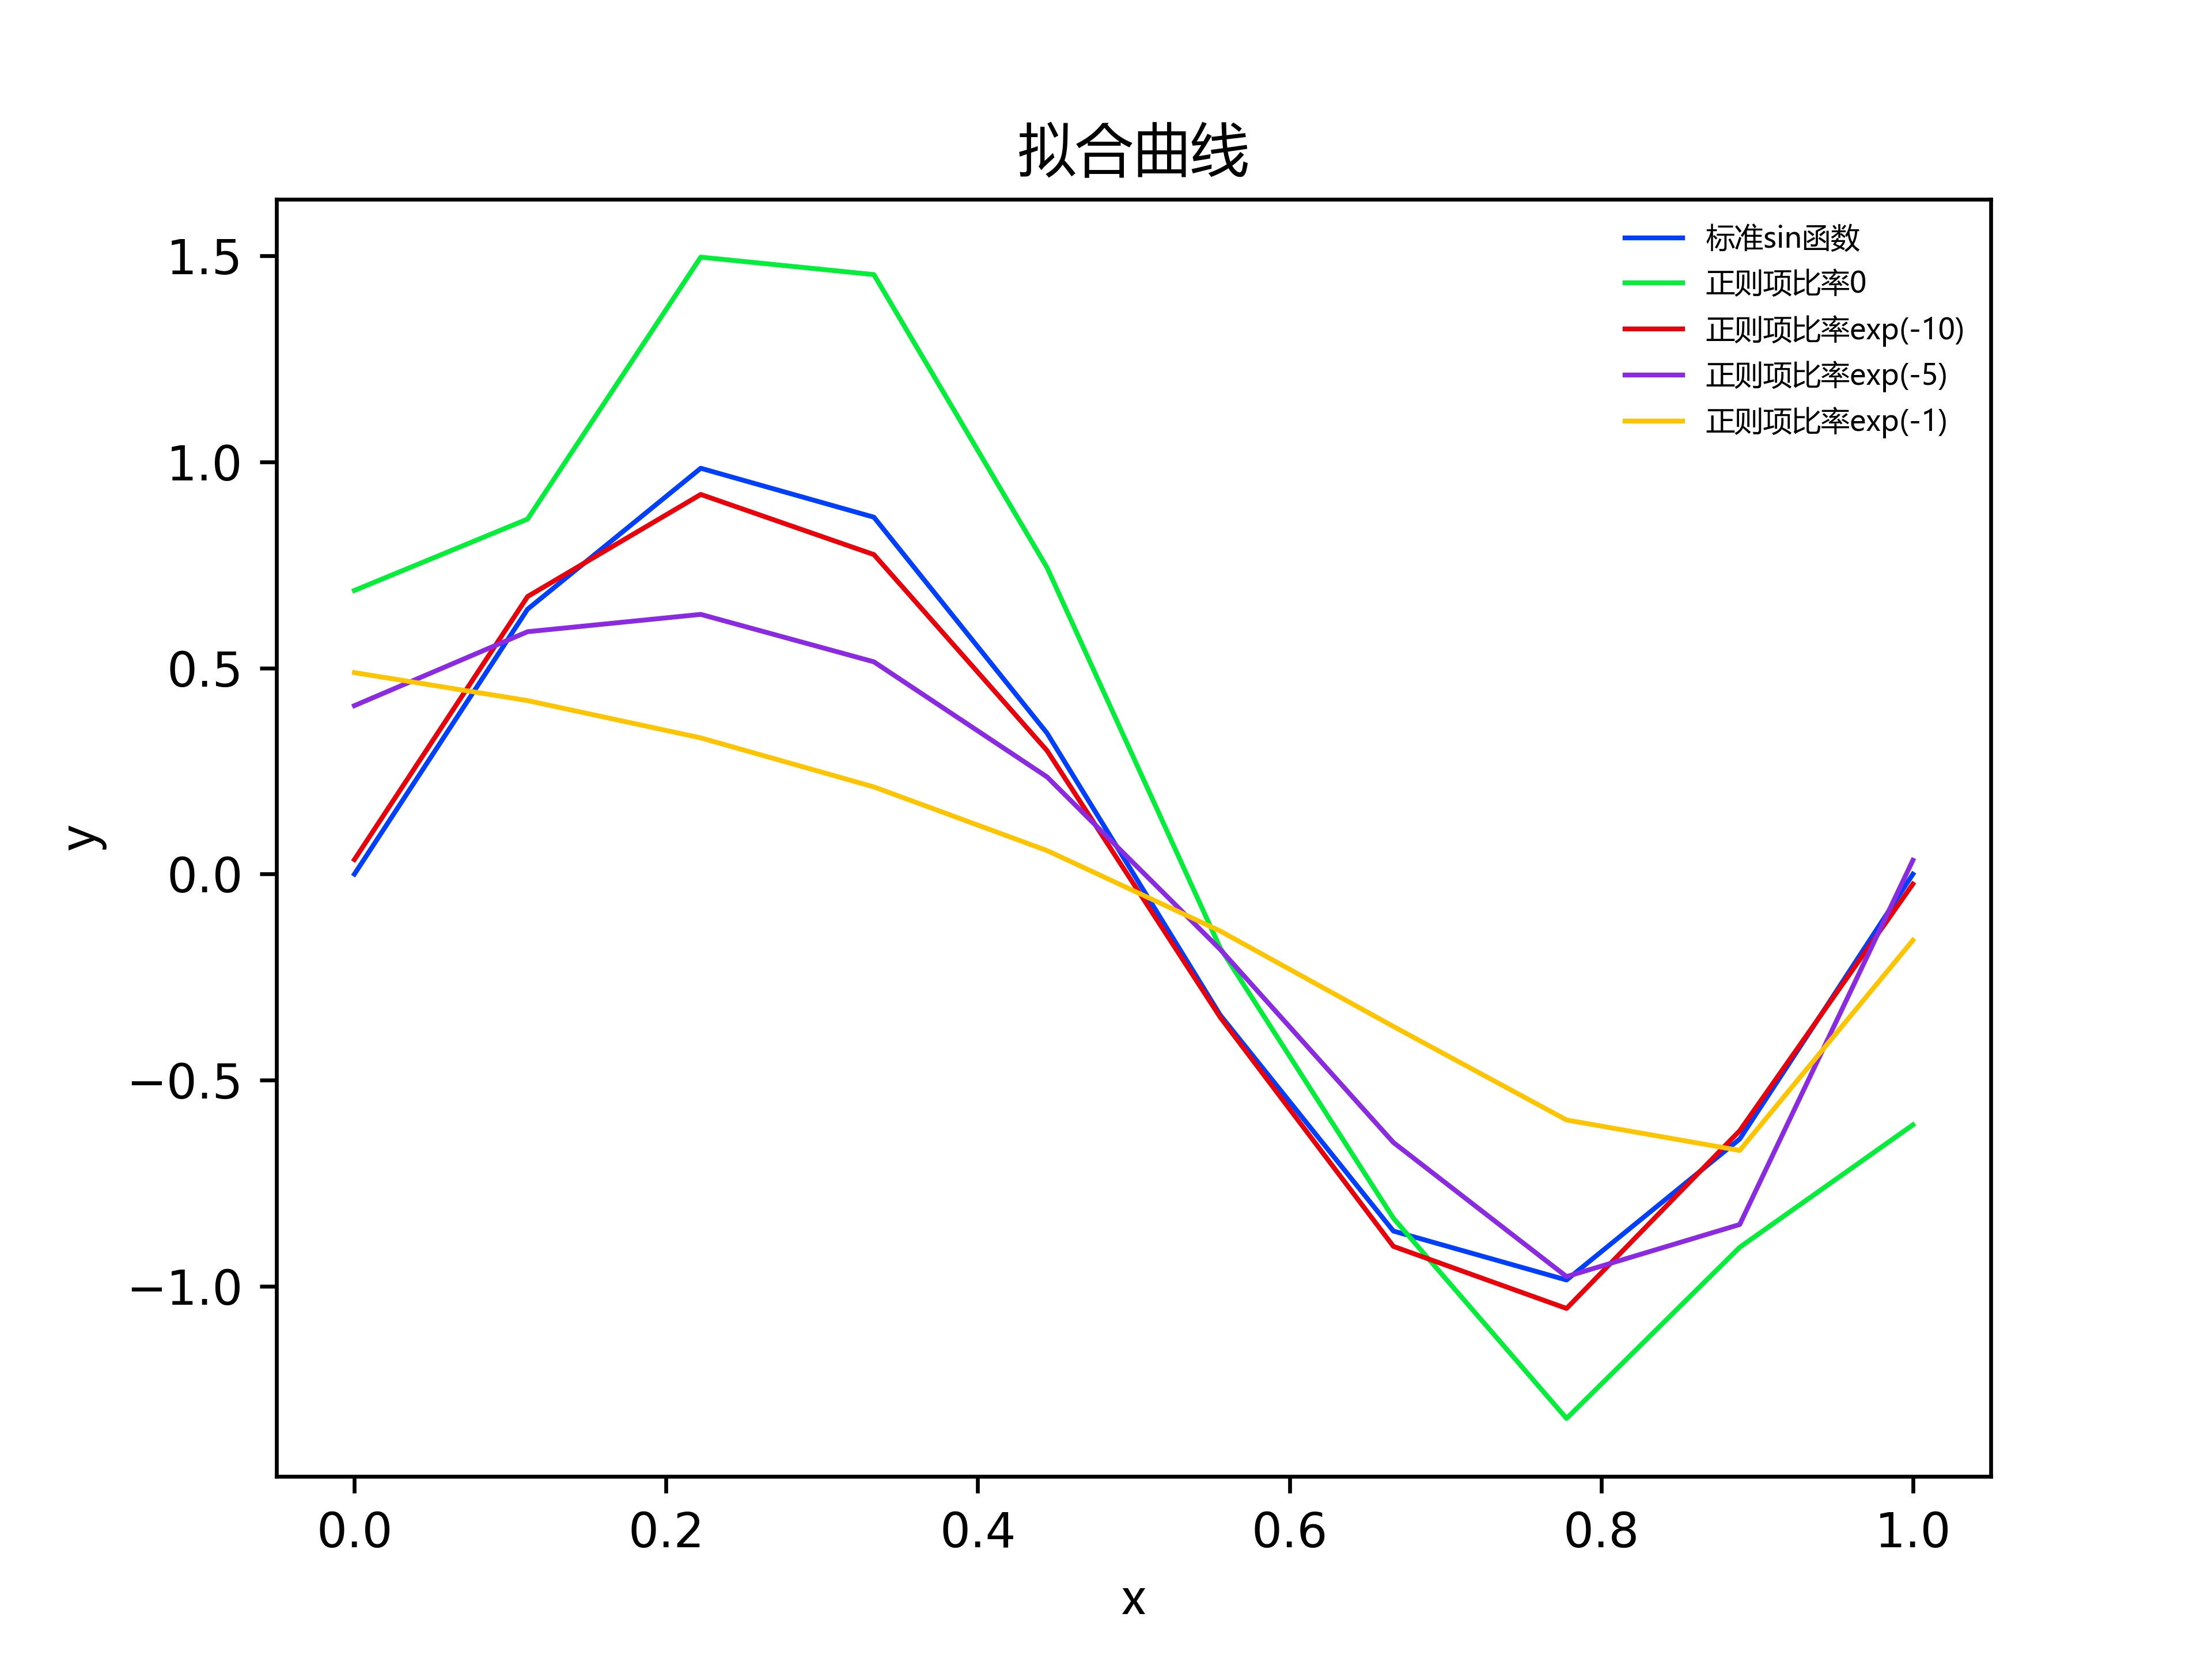
\includegraphics[width=0.88\textwidth]{n10o12正则项系数}
    \caption{不同正则项系数下拟合曲线}
    \label{图5}
\end{figure}

由上图可以看出正则项系数为0,即不带正则项的情况下曲线波动较大,甚至部分点取值大于1。通过调试可得,此时由于加入了噪声,训练集数据中的确出现了标记值大于1的情况,因阶数高拟合能力强,且无正则项减少震荡,导致模型将训练集中噪声作为了所有样本都具有的特点,也由此与标准$sin$函数差距较大。

\subsection{补充:50阶下拟合效果}
根据实验要求,补充解析解,带优化的梯度下降,共轭梯度法在$n=100$、$m=50$的情况如下。
\linespread{1.2}
\begin{table}[H]
\centering
\caption{n=100 m=50拟合优度}
\label{tab:performance_comparison}  %可能是自动编号
\begin{tabular}{ccccc} %cc表示有两行,中见加|,则表格中就会多一条竖线
\toprule[1.5pt] %加粗
 \makebox[0.17\textwidth][c]{方法}	&  \makebox[0.17\textwidth][c]{解析法} &  \makebox[0.17\textwidth][c]{梯度下降} &  \makebox[0.17\textwidth][c]{Adam优化梯度下降}
&  \makebox[0.17\textwidth][c]{共轭梯度法}\\ \hline
拟合优度&10.6364&0.0821&0.0400&0.0396  \\
\bottomrule[1.5pt] %加粗
\end{tabular}
\end{table}

\begin{figure}[H]
    \centering
    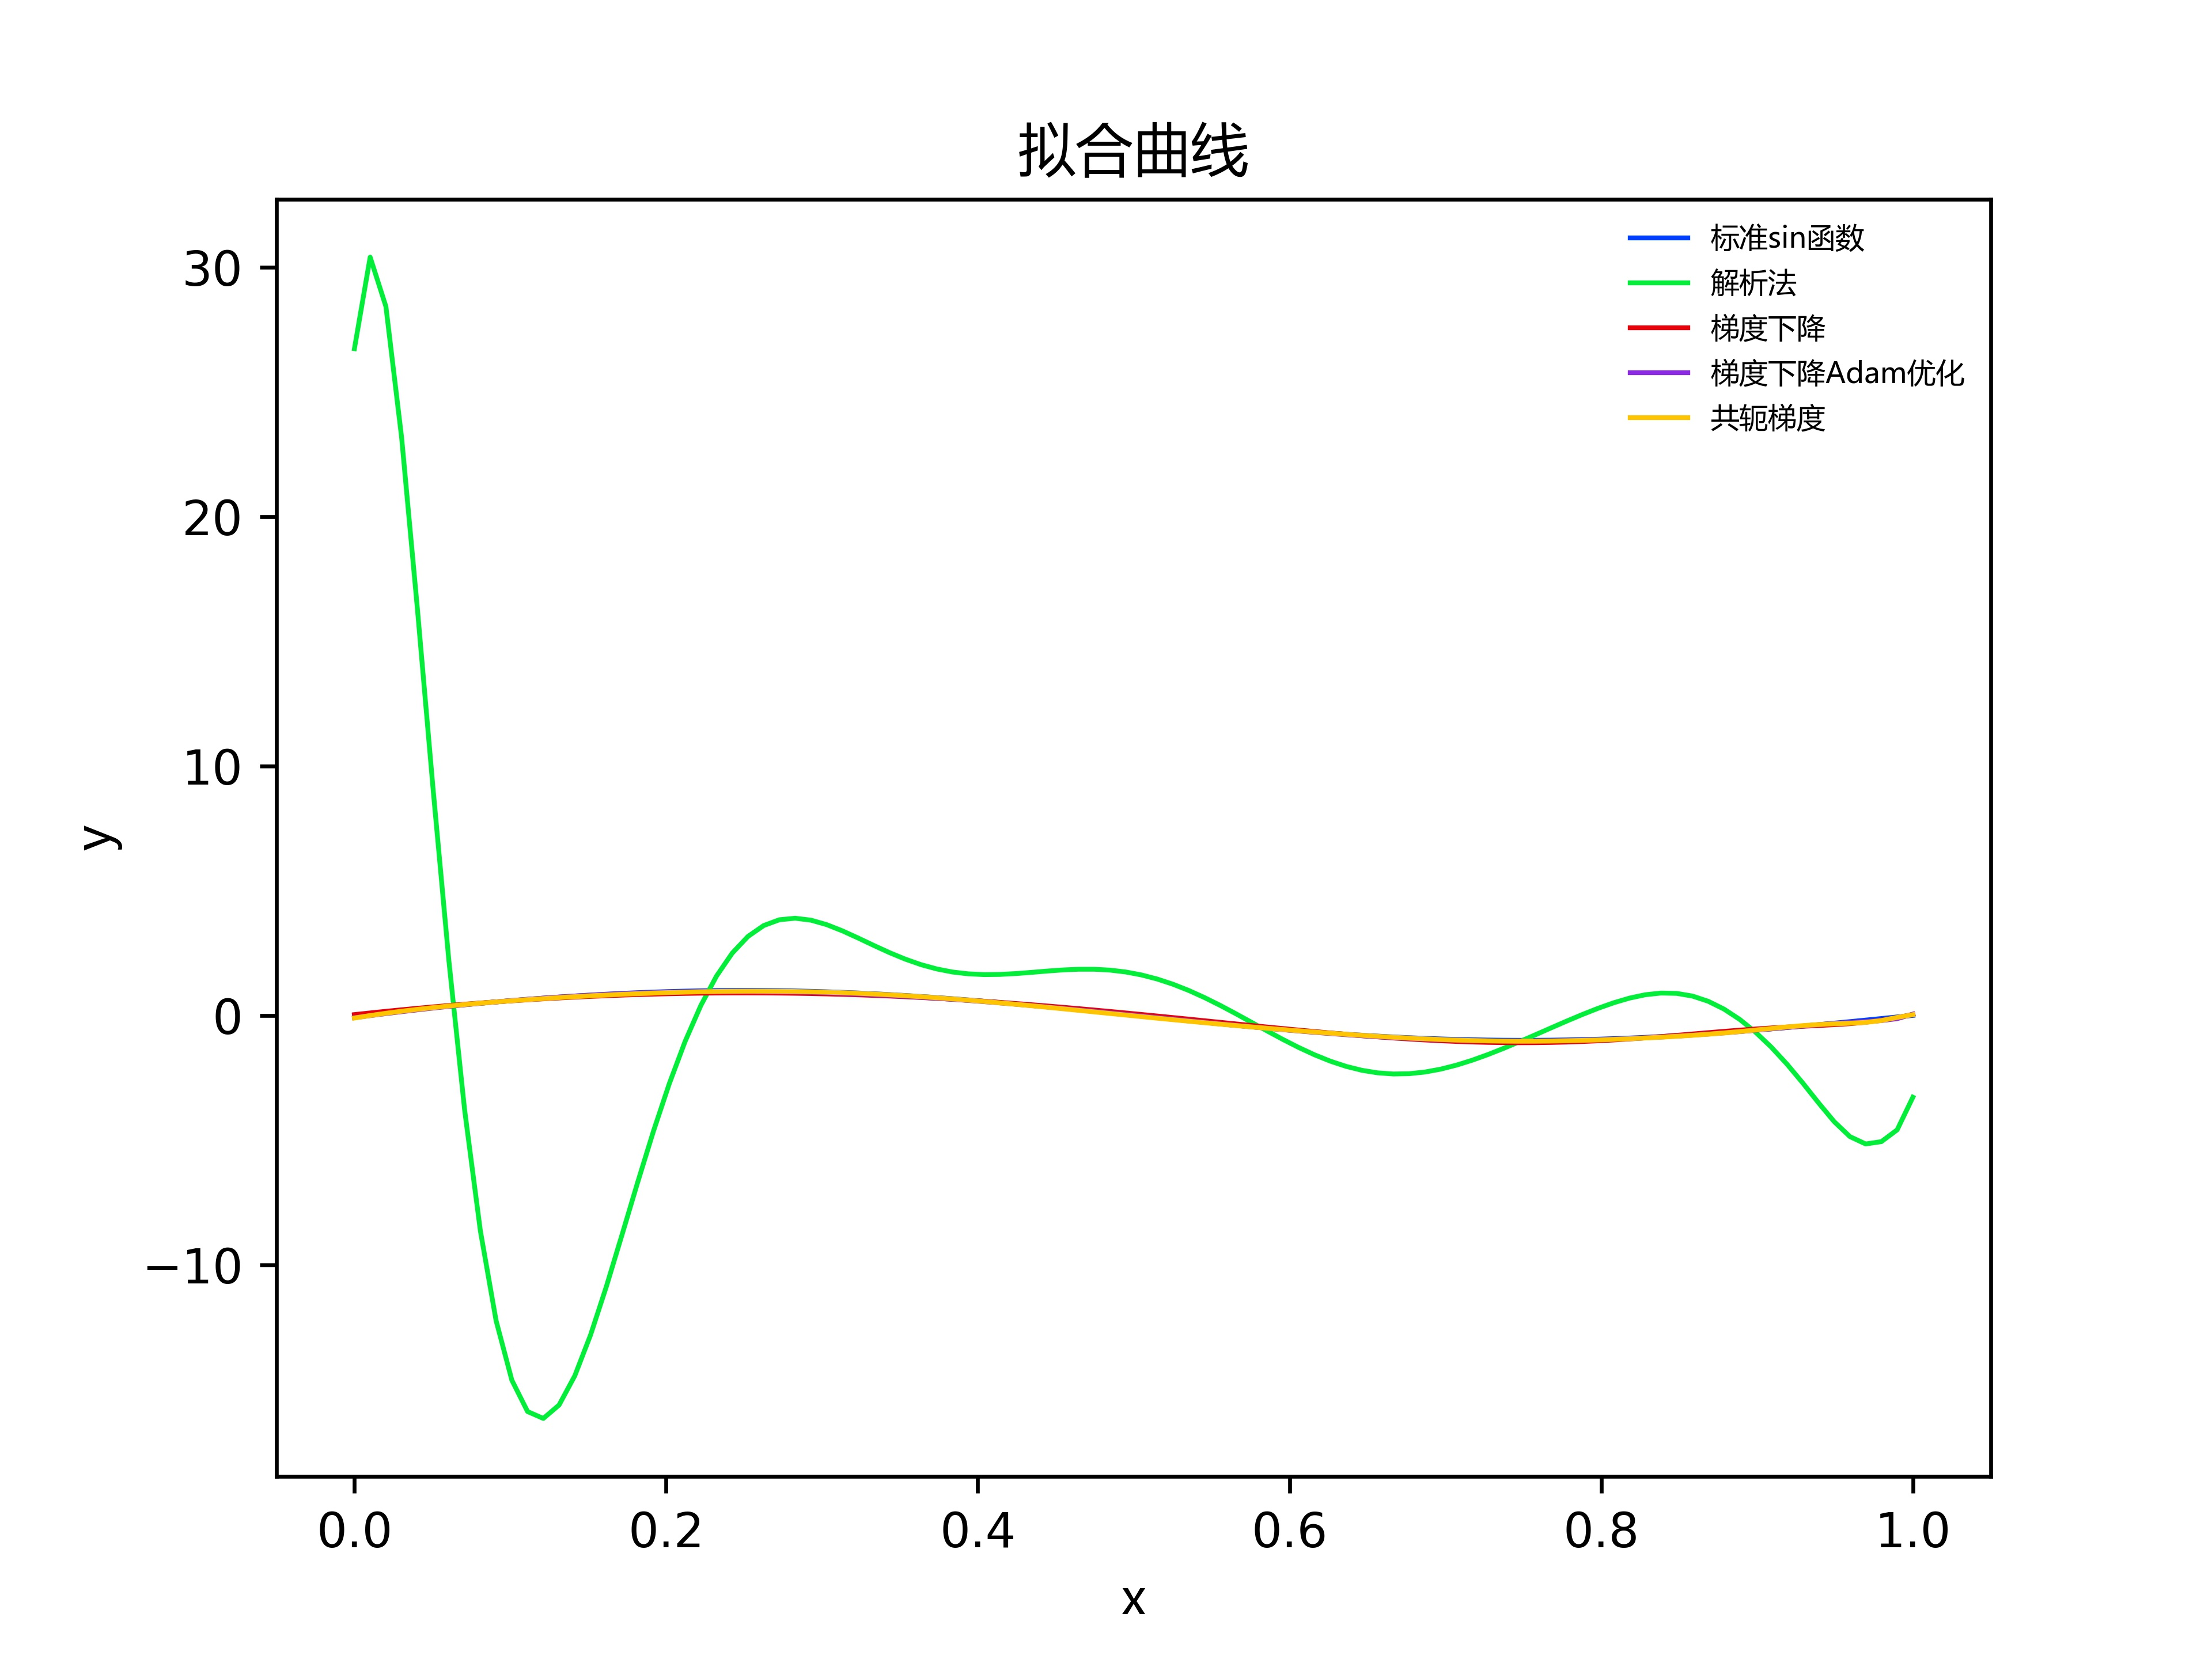
\includegraphics[width=0.88\textwidth]{n100o50}
    \caption{n=100 m=50拟合曲线}
    \label{图6}
\end{figure}

观察可得,此时解析法拟合效果效果已彻底崩溃,但根据相同的解析式算出的梯度和解,使用其他的方法,拟合效果仍保持不变,故可以猜测是Python内部算法存在问题,可能性最大的便是numpy库中的求逆函数。

此时梯度下降未优化和优化后的用时分别为20497ms和850ms。

\section{结论}
拟合次数较小时,函数拟合能力不强,误差较大。次数过大时则会产生过拟合现象,曲线波动较大。过拟合可以使用加入正则项的方法消除。正则项参数过大会导致拟合曲线过于平缓,过小则会导致消除过拟合效果不好。


\begin{thebibliography}{1}
\bibitem{wiki}
Wikipedia,
https://en.wikipedia.org/wiki/Conjugate\_gradient\_method,
last accessed 2021/09/26
\end{thebibliography}

\newpage
\begin{appendix}
\section{主程序}
\begin{lstlisting}[language=python]
import copy
import math

import matplotlib.pyplot as plt
import numpy as np
import random
from graph import init_graph, draw_graph

# 数据集大小
num = 50
# 多项式次数
order = 9
# 梯度下降学习率
learning_rate = 0.01
# 正则项比率
regulation_radio = np.exp(-5)
# 梯度下降停止条件
gradient_descent_epsilon = 1e-7
# 使用Adam加速的梯度下降停止条件
gradient_descent_adam_epsilon = 1e-7
# 共轭梯度停止判断条件
conjugate_gradient_epsilon = 1e-10


# 解析法
def analytic_method(X, y):
    return np.dot(np.matmul(np.linalg.inv(np.matmul(np.transpose(X), X)), np.transpose(X)), y)


# 解析法+正则项
def analytic_method_regulation(X, y):
    return np.dot(np.matmul(np.linalg.inv(np.matmul(np.transpose(X), X) + np.identity(order + 1, dtype=int) * regulation_radio), np.transpose(X)), y)


# 梯度下降
def gradient_descent_batch(X, y):
    w = np.array([1.0 for _ in range(order + 1)])
    while True:
        gradient = np.dot(np.transpose(X), np.dot(X, w) - y) / num
        if np.dot(np.transpose(gradient), gradient) < gradient_descent_epsilon:
            break
        for i in range(10000):
            gradient = np.dot(np.transpose(X), np.dot(X, w) - y) / num
            w -= learning_rate * gradient
    return w


# 梯度下降Adam方法
def gradient_descent_adam(X, y):
    # adam中的超参数,一般使用以下值
    adam_beta_1 = 0.9
    adam_beta_2 = 0.99
    inf_small = 1e-8

    # 计算过程中的累计值
    m = np.zeros(order + 1)
    v = np.zeros(order + 1)
    accumulative_adam_beta_1 = adam_beta_1
    accumulative_adam_beta_2 = adam_beta_2

    w = np.array([1.0 for _ in range(order + 1)])

    while True:
        gradient = np.dot(np.transpose(X), np.dot(X, w) - y) / num
        if np.dot(np.transpose(gradient), gradient) < gradient_descent_adam_epsilon:
            break

        for i in range(10000):
            gradient = np.dot(np.transpose(X), np.dot(X, w) - y) / num
            m = adam_beta_1 * m + (1 - adam_beta_1) * gradient
            v = adam_beta_2 * v + (1 - adam_beta_2) * (gradient ** 2)
            M = m / (1 - accumulative_adam_beta_1)
            V = v / (1 - accumulative_adam_beta_2)
            accumulative_adam_beta_1 *= adam_beta_1
            accumulative_adam_beta_2 *= adam_beta_2
            w -= learning_rate * M / (V ** (1 / 2) + inf_small)

    return w


# 参考https://en.wikipedia.org/wiki/Conjugate_gradient_method中伪代码
# 共轭梯度
def conjugate_gradient_method(X, y):
    w = np.array([1.0 for _ in range(order + 1)])
    A = np.matmul(np.transpose(X), X)
    b = np.dot(np.transpose(X), y)
    r = b - np.dot(A, w)

    if np.dot(np.transpose(r), r) < conjugate_gradient_epsilon:
        return w

    p = copy.deepcopy(r)

    while True:
        alpha = np.dot(np.transpose(r), r) / np.dot(np.dot(np.transpose(p), A), p)
        w += alpha * p
        temp = copy.deepcopy(r)
        r -= alpha * np.dot(A, p)

        if np.dot(np.transpose(r), r) < conjugate_gradient_epsilon:
            break

        beta = np.dot(np.transpose(r), r) / np.dot(np.transpose(temp), temp)
        p = r + beta * p

    return w


if __name__ == '__main__':
    x = np.linspace(0, 1, num, endpoint=True, dtype=float)
    y_raw = np.array(np.sin(2 * np.pi * x))
    # 加入噪声
    y = np.array([y_raw[i] + random.gauss(0, 1) / 10 for i in range(num)])
    # 得到设计的矩阵X
    X = np.array([x[i // (order + 1)] ** (i % (order + 1)) for i in range(num * (order + 1))]).reshape(num, order + 1)

    init_graph("x", "y", "拟合曲线", dpi=600)
    plt.plot(x, y_raw, linewidth=1, label="标准sin函数")

    # 求多项式参数
    w1 = analytic_method(X, y)
    w2 = analytic_method_regulation(X, y)
    w3 = gradient_descent_batch(X, y)
    w4 = gradient_descent_adam(X, y)
    w5 = conjugate_gradient_method(X, y)

    # 求拟合曲线
    y1 = np.dot(X, w1)
    y2 = np.dot(X, w2)
    y3 = np.dot(X, w3)
    y4 = np.dot(X, w4)
    y5 = np.dot(X, w5)

    plt.plot(x, y1, linewidth=1, label="解析法")
    plt.plot(x, y2, linewidth=1, label="解析法+正则项")
    plt.plot(x, y3, linewidth=1, label="梯度下降")
    plt.plot(x, y4, linewidth=1, label="梯度下降Adam优化")
    plt.plot(x, y5, linewidth=1, label="共轭梯度")

    print("解析法:", w1, "拟合优度:", math.sqrt(np.dot(np.transpose(y1 - y_raw), y1 - y_raw) * 2 / num))
    print("解析法+正则项:", w2, "拟合优度:", math.sqrt(np.dot(np.transpose(y2 - y_raw), y2 - y_raw) * 2 / num))
    print("梯度下降:", w3, "拟合优度:", math.sqrt(np.dot(np.transpose(y3 - y_raw), y3 - y_raw) * 2 / num))
    print("梯度下降Adam优化", w4, "拟合优度:", math.sqrt(np.dot(np.transpose(y4 - y_raw), y4 - y_raw) * 2 / num))
    print("共轭梯度:", w5, "拟合优度:", math.sqrt(np.dot(np.transpose(y5 - y_raw), y5 - y_raw) * 2 / num))
    
    draw_graph(legend=True, save=True, filename="测试.jpg")

\end{lstlisting}

\section{可视化}
\begin{lstlisting}[language=python]
from matplotlib import pyplot as plt

# 设置字体,解决中文无法识别的问题
# 图表标题
font_title = {
    'family': 'Microsoft Yahei',
    'weight': 'regular',
    'size': 12
}

# 坐标轴标题
font_label = {
    'family': 'Microsoft Yahei',
    'weight': 'regular',
    'size': 10
}

# 图例
font_legend = {
    'family': 'Microsoft Yahei',
    'weight': 'regular',
    'size': 6
}


def init_graph(xlabel, ylabel, title, dpi=150, style="seaborn-bright"):
    # 设置清晰度
    plt.figure(dpi=dpi)

    # 设置样式
    plt.style.use(style)

    # 添加x,y轴名称
    plt.xlabel(fontdict=font_label, xlabel=xlabel)
    plt.ylabel(fontdict=font_label, ylabel=ylabel)

    # 添加标题
    plt.title(title, font=font_title)


def draw_graph(legend=False, save=False, filename="picture.jpg", show=False):
    # 是否添加图例
    if legend:
        plt.legend(prop=font_legend, loc='upper right', frameon=False)

    # 是否保存
    if save:
        plt.savefig("./figures/" + filename)

    if show:
        plt.show()
\end{lstlisting}
\end{appendix}
\end{document}